\documentclass[12pt, openany]{cmuthesis}

\usepackage{newtxtext, newpxmath}
\usepackage[T1]{fontenc} 
\usepackage{graphicx}
\graphicspath{{./}{tutorial/plots/}}
\usepackage{tikz}
\usetikzlibrary{positioning}
\usepackage{enumitem}
\usepackage{comment}
\usepackage{amsmath}
\usepackage{listings}
\usepackage{booktabs}
\usepackage{adjustbox}
\usepackage[skins]{tcolorbox}
\usepackage{fontawesome}
\usepackage{multirow}
\usepackage{wrapfig}
\usepackage{calc}
\usepackage{xspace}
\usepackage{subcaption}
\usepackage{minted}
\usepackage{balance}
\usepackage{threeparttable}
\usepackage{makecell}
\usepackage{framed}
\usepackage[backend=biber, style=numeric]{biblatex}\let\citet\textcite\let\citep\parencite
\usepackage[letterpaper,twoside,vscale=.8,hscale=.75,nomarginpar,hmarginratio=1:1]{geometry}
\usepackage[
    pageanchor=true,
    plainpages=false,
    pdfpagelabels, 
    bookmarks,
    bookmarksnumbered, 
    hidelinks
]{hyperref}

%%%%%%%%%% Begin: JSON Syntax Definition %%%%%%%%%%
\makeatletter
% switch used as state variable
\newif\ifcolonfoundonthisline
\newcommand\JSONnumbervaluestyle{\color{blue!80!black}}
\newcommand\JSONstringvaluestyle{\color{red!80!black}}
\lstdefinestyle{json}{
  showstringspaces    = false,
  keywords            = {false,true},
  alsoletter          = 0123456789.,
  morestring          = [s]{"}{"},
  stringstyle         = \ifcolonfoundonthisline\JSONstringvaluestyle\fi,
  MoreSelectCharTable = \lst@DefSaveDef{`:}\colon@json{\processColon@json},
  basicstyle          = \footnotesize\ttfamily\linespread{0.5},
  keywordstyle        = \ttfamily\bfseries,
  numbers             = left,
  numberstyle         = \scriptsize,
  stepnumber          = 1,
  numbersep           = 6pt,
  showstringspaces    = false,
  breaklines          = true,
  frame               = lines,
  escapeinside        = {(*}{*)}
}
% flip the switch if a colon is found in Pmode
\newcommand\processColon@json{%
  \colon@json%
  \ifnum\lst@mode=\lst@Pmode%
    \global\colonfoundonthislinetrue%
  \fi
}
\lst@AddToHook{Output}{%
  \ifcolonfoundonthisline%
    \ifnum\lst@mode=\lst@Pmode%
      \def\lst@thestyle{\JSONnumbervaluestyle}%
    \fi
  \fi
  %override by keyword style if a keyword is detected!
  \lsthk@DetectKeywords% 
}
% reset the switch at the end of line
\lst@AddToHook{EOL}{\global\colonfoundonthislinefalse}
%%%%%%%%%% End:   JSON Syntax Definition %%%%%%%%%%

%%%%%%%%%% Begin: Finding Box Definition %%%%%%%%%%
\tcbset{
  my box2/.style={
    enhanced,
    colframe=#1!80,
    colback=#1!5,
  },
}
\newtcolorbox{finding}{
  my box2=black,
  boxrule=1pt,top=3pt,bottom=3pt,left=4pt,right=4pt
}
\newtcolorbox{summary-rq}{
  my box2=black,
  boxrule=1pt,top=3pt,bottom=3pt,left=4pt,right=4pt
}
%%%%%%%%%% End:   Finding Box Definition %%%%%%%%%%

%%%%%%%%%% Begin: Custom Commands and Colors %%%%%%%%%%
\renewcommand*{\ttdefault}{lmtt} % Change texttt font

\newcommand{\TODO}[1]{{\textbf{\color{red}[[TODO: #1]]}}}
\newcommand{\Code}[1]{\texttt{#1}}
\newcommand{\SmallCode}[1]{\begin{small}\texttt{#1}\end{small}}
\newcommand{\SystemName}[0]{\texttt{StarScout}\xspace}
\newcommand{\RQOne}[0]{\textbf{RQ1} (\textsf{Prevalence}): \emph{How prevalent are fake GitHub stars?}\xspace}
\newcommand{\RQTwo}[0]{\textbf{RQ2} (\textsf{Activity Patterns}): \emph{What are the activity patterns of GitHub repositories and accounts with fake star campaigns?}}
\newcommand{\RQThree}[0]{\textbf{RQ3} (\textsf{Repository Characteristics}): \emph{What are the GitHub repositories with fake star campaigns?}}
\newcommand{\RQFour}[0]{\textbf{RQ4} (\textsf{Promotional Effect}): \emph{To what extent are fake stars effective in promoting the target GitHub repositories?}}
\newcommand{\numtreated}{806\xspace}

\definecolor{darkred}{rgb}{0.9, 0.0, 0.0}
\definecolor{darkgreen}{rgb}{0.0, 0.8, 0.0}
\definecolor{amber}{rgb}{1.0, 0.75, 0.0}
%%%%%%%%%% End: Custom Commands and Colors %%%%%%%%%%

\addbibresource{references.bib}
\addbibresource{references-pinning.bib}
\addbibresource{references-fake-stars.bib}
\addbibresource{references-cursor.bib}
\addbibresource{tutorial/paper/references.bib}

\begin{document}
\frontmatter

\pagestyle{empty}

\title{{\it Thesis}\\
{\bf Dispelling Software Engineering Myths:\\A Pragmatic Causal Inference Approach
}}
\author{Hao He}
\date{\today}
\Year{\the\year}
\trnumber{}

\committee{
Bogdan Vasilescu, Co-Chair \\
Christian Kästner, Co-Chair \\
Rohan Padhye \\
Narayan Ramasubbu
}

%\support{This work was supported in part by the National Science Foundation (award 2206859).}
%\disclaimer{The views expressed in this work are those of the author and do not necessarily reflect the views of the sponsoring agencies.}

\keywords{causal inference, empirical software engineering, mining software repositories, research methodology, quasi-experimental design, observational studies, AI coding tools, software supply chain security, GitHub, developer productivity, open-source software}

\maketitle

%\begin{dedication}
%For my dog
%\end{dedication}

\pagestyle{plain} % for toc, was empty

\begin{abstract}
Software engineering practice is filled with myths---beliefs derived from intuition, experience, and conventional wisdom---that lack empirical foundations.
Many of these myths are \emph{causal} in nature, concerning the consequences of decisions, interventions, and changes to practice.
While empirical software engineering research frequently investigates these myths through descriptive, correlational, and qualitative evidence, it rarely engages with the challenging question of \emph{whether} the evidence can actually support the causal claims beneath these myths.
In this thesis, I argue that \emph{causal credibility assessments are feasible in empirical software engineering research through explicit articulations of causal theory and assumptions}.

To demonstrate this argument, this thesis starts with an accessible introduction to the modern causal inference toolkit for software engineering researchers.
I will cover three conceptual pillars that would enable explicit articulations of causal theory and assumptions in empirical settings: potential outcomes framework, graphical causal models, and design-based identification.
I will walk through AI coding tool adoption as a running example throughout, demonstrating how progressively stronger causal research designs can be made through articulating a causal theory and inspecting the plausibility of assumptions beneath each statistical method used.

Then, across three empirical studies, I demonstrate how causal credibility assessments can reveal systematic gaps between practitioner beliefs and empirical reality. 
First, using counterfactual analysis and simulations on npm dependency data, I challenge the myth that pinning dependency versions improves project security, showing that it paradoxically increases attack exposure unless upstream packages pin their own dependencies. 
Second, through a longitudinal analysis of GitHub starring patterns with panel regression models, I challenge the myth that fake GitHub stars provide sustainable promotional benefits, showing instead that these artificial signals become long-term liabilities. 
Finally, using a difference-in-differences design with staggered adoption, I challenge the myth that AI coding tools unambiguously improve developer productivity, finding that Cursor's initial velocity gains are offset by sustained accumulation of technical debt.
In each study, I assess the credibility of causal claims through the following four-step framework: (1) deriving an explicit causal theory from software engineering domain knowledge, (2) defining the causal estimate of interest and specifying the assumption under which the estimate carries a causal interpretation, (3) honestly acknowledging and mitigating limitations and known caveats, and (4) thoughtfully navigating alternative explanations.
Collectively, this thesis provides a methodological blueprint for future empirical software engineering research, illustrating how to balance rigor with practicality to generate actionable, trustworthy evidence for software engineering myths.
\end{abstract}

\begin{acknowledgments}
First and foremost, I am profoundly indebted to my advisors, Bogdan Vasilescu and Christian Kästner, whose guidance has shaped almost every facet of my research---from the questions I have learned to ask to the standards I now hold myself to.
None of what this thesis represents would have been possible without their patience, mentorship, and unwavering support.
Also, I am deeply grateful to my thesis committee members and research collaborators---Narayan Ramasubbu, Rohan Padhye, Alexandros Kapravelos, Philipp Burckhardt, Courtney Miller, Shyam Agarwal, and Haoqin Yang---whose insights and contributions are woven through the work presented in this thesis.
Last but not least, I am grateful to James Herbsleb, Vladimir Filkov, Audris Mockus, Laurie Williams, Patrick Park, Shurui Zhou, Alexandra Xinran Li, Yining She, Yining Hong, Chenyang Yang, Haoze He, and all participants of the S3C2 quarterly meetings for the conversations, feedback, and generous help that have accompanied me throughout my PhD journey at Carnegie Mellon University.

I would like to give a special thanks to my former PhD advisor, Minghui Zhou, at Peking University.
Minghui's generous support of me reapplying for the PhD program at CMU was truly a selfless act that I will never forget.
I would also like to thank my past collaborators when I was working at Peking University---Yuxia Zhang, Runzhi He, Weiwei Xu, Wenxin Xiao, Kai Gao, Jinhao Dong, Jianyu Wu, Xin Tan, Haiqiao Gu, Yifei Xu, Chao Wang---for their valuable contributions to my past research projects which helped me grow as a researcher.

To my partner and my parents, I owe a debt I cannot repay.
Thank you for an understanding without parallel, both for what this work has demanded of me and for the rest of life beyond it.
These years have not always been easy, and the PhD itself, in honesty, was rarely the hardest part.
I owe a quieter gratitude to the other life hardships I faced in parallel, too, for making me stronger, more resilient, and more attuned to the blessings I am fortunate to hold in my current life.

The work in this thesis was supported in part by the National Science Foundation under award 2206859 (Kästner) and award 2317168 (Vasilescu), as well as research awards to Vasilescu from Google and the Digital Infrastructure Fund.
The work in Chapter~\ref{chp:fake-stars} was further supported in part by the National Science Foundation under award 2207008 (Kapravelos).
The work in Chapter~\ref{chp:fake-stars} is also supported by Socket Inc (\url{https://socket.dev}) and its CEO, Feross Aboukhadijeh, for the collaboration opportunities, general support, and computational resources that made the work in Chapter~\ref{chp:fake-stars} possible.
The work in Chapter~\ref{chp:cursor} was further supported by the National Science Foundation Graduate Research Fellowship Program under Grant Number DGE214073 (Miller). 
Finally, I thank the Google Cloud for Researchers program for the credits that funded the BigQuery-based analyses in Chapters~\ref{chp:fake-stars} and~\ref{chp:cursor}.
\end{acknowledgments}

\tableofcontents

%\listoffigures

%\listoftables

\mainmatter

\chapter{Introduction}
\label{chp:intro}

\section{Motivation}

Software engineering is among the most consequential engineering disciplines of the modern era. 
Software systems underpin critical infrastructure across healthcare, finance, transportation, and communication, with failures potentially affecting millions of users, costing billions of dollars, and projecting real-world consequences~\cite{eghbal2016roads, solar-wind, xz-attack}. 
The decisions software engineers make, and the practices they adopt daily (e.g., dependency management strategies, tool adoption choices), accumulate into system-wide outcomes that shape organizational productivity, security posture, and long-term maintainability. 
Given these stakes, one might expect software engineering practice to be grounded in rigorous, evidence-based principles analogous to those in medicine~\cite{sackett1996evidence} or civil engineering~\cite{petroski1985engineer}. 
Unfortunately, this expectation remains largely unfulfilled.

In fact, software engineering practice today is characterized more by folklore, intuition, and contested conventional wisdom than by empirically validated guidance~\cite{DBLP:conf/icse/Devanbu0B16, DBLP:journals/ese/GarousiBO20, DBLP:journals/ese/ShrikanthNFM21, enoiu2026folklore}. 
While practitioners face consequential decisions on a routine basis, they very often find limited reliable evidence to inform their choices. 
To support their decisions, they draw on their own experiences or navigate a landscape of blog posts, podcasts, and conference talks to learn opinions of the ``said'' experts. 
This decision-making process is largely ad hoc, lacks empirical foundations, and may or may not lead to a consensus in the field.
As a result, the field abounds with what I may call \textbf{software engineering myths}, which are \emph{widely held beliefs about best practices derived from intuition, experience, and conventional wisdom, that have never been rigorously tested or, when tested, have produced inconclusive or contradictory results}.

This state of affairs persists despite decades of empirical research in software engineering. 
The field has generated thousands of studies examining key software engineering topics, including developer productivity, code quality, security practices, and the effectiveness of developer tools. 
It has also embraced a vast body of empirical methodological frameworks over the past decades, such as randomized controlled experiments~\cite{DBLP:books/sp/WohlinRHORW24}, discussion of internal/external validity and its trade-offs~\cite{DBLP:conf/icse/SiegmundSA15, DBLP:journals/tosem/RobillardAEGLNNSSS24}, open-science~\cite{DBLP:books/sp/20/0001G0S20}, registered reports~\cite{DBLP:journals/ese/ErnstB23}, qualitative synthesis~\cite{DBLP:conf/esem/CruzesD11}, and more.
This diversity is most apparent in the ACM SIGSOFT Empirical Standards, offering method-specific checklists for 19 major software engineering research methods~\cite{DBLP:journals/corr/abs-2010-03525}.

Despite this substantial body of work, software engineering remains a field with a high degree of folklore, intuition, and conventional wisdom, rather than an evidence-based discipline.
Why is this the case?
There are for sure many unique challenges in the field of empirical software engineering, such as the lack of accurate measurements for key constructs~\cite{DBLP:conf/ease/RalphT18}, the vast ecological diversity of software systems~\cite{DBLP:conf/sigsoft/NagappanZB13}, and the rapid moving nature of software engineering practices in general.
Apart from these challenges, I want to note one important blocker: Many of the software engineering myths we see in practice are \emph{causal in nature}---concerning the effect of an intervention on an outcome of interest---but empirical SE research rarely engages with the challenging question of \emph{whether the presented evidence can actually support a causal claim, and to what extent}.
Instead, researchers often approach software engineering myths with either: (a) descriptive and statistical modeling from software repository data, with a blanket disclaimer that the observed correlation does not imply causation, or (b) qualitative evidence synthesizing and interpreting practitioner opinions on the topic of interest.
Neither would provide sufficient evidence to support or dispel a software engineering myth, especially when it is contested.

For example, consider the following problem: Should software projects allow flexibility in the versions of their dependencies, and to what extent?
A descriptive mining software repository study~\cite{DBLP:conf/msr/0001PSTB19} may conclude that the Java/Maven ecosystem is extensively pinning dependency versions while the JavaScript/npm ecosystem is extensively using semantic versioning, without providing any concrete guidance or discussions of the trade-offs around them.
A qualitative study surveying JavaScript developers~\cite{DBLP:journals/tse/JafariCAST22} may conclude that semantic versioning should be preferred over pinned dependencies as the latter is a ``dependency smell'' likely to cause maintainability issues in the future.
Another qualitative study interviewing security experts~\cite{DBLP:conf/sp/LadisaPMB23} may conclude that dependency pinning should be preferred over semantic versioning, as the former is critical for preventing software supply chain attacks.
In this case, the quantitative repository mining study fails to provide evidence-based guidance, while the two qualitative studies present contradictory opinions from practitioner cohorts with different experiences and perspectives; neither would be sufficient to formulate best practices for this dependency versioning problem.

Similarly, consider the longstanding debate over whether the choice of programming language causally affects defect-proneness. 
A large-scale correlational study~\cite{DBLP:conf/sigsoft/RayPFD14, DBLP:journals/cacm/RayPDF17} analyzed millions of commits across thousands of GitHub projects; the study concluded that programming language has a significant but modest effect on defect-proneness, with functional and statically-typed languages associated with fewer defects.
However, a reproduction study~\cite{DBLP:journals/toplas/BergerHMVV19} revisiting the same dataset with methods that they claim to be better---correcting errors in language classification, accounting for polyglot repositories, and applying more appropriate statistical models---found that the original effect sizes shrank dramatically and many findings failed to replicate. 
The original authors issued a rebuttal~\cite{DBLP:journals/corr/abs-1911-07393} defending their methodology, which prompted a counter-rebuttal~\cite{DBLP:journals/corr/abs-1911-11894} from the reproduction team. 
Putting the controversy around the specific research design aside, the counter-rebuttal~\cite{DBLP:journals/corr/abs-1911-11894} reveals a deeper methodological impasse behind why the field cannot reach consensus on a seemingly straightforward empirical question:
\begin{quote}
\emph{I fundamentally do not believe that the question the FSE authors set out to answer, namely, whether some languages are more defect-prone than others, can be meaningfully answered by scraping GitHub...An analysis of GitHub is necessarily measuring correlation and not establishing causation, as it does not constitute an experiment.}
\end{quote}

The problem extends beyond individual studies and renders empirical software engineering research particularly unproductive on contested problems in which practitioners have strong and conflicting intuitions and beliefs.
When studies only repeat and synthesize practitioner opinions, it may be biased towards a specific perspective and may not be sufficient to shift the posterior beliefs of others.
When studies finds certain correlations from observational data, practitioners will naturally want to read the study as causal without considering the limitations of the study design and the potential confounding factors.
Even worse, when studies reach controversial conclusions (which may be extremely valuable if carefully justified) but fail to rule out important confounding factors or alternative explanations, practitioners may become skeptical of the field altogether. 
The result is a field with prevalent myths despite plentiful empirical research.

Modern causal inference methods offer a principled approach to addressing this problem~\cite{cunningham2021causal, pearl2009causality, hansen2022econometrics}. 
Developed primarily in econometrics and epidemiology over the past several decades, these methods provide frameworks for distinguishing genuine causal effects from spurious correlations in observational data---precisely the kind of data investigated in repository mining studies.
Importantly, the value of causal inference methods lies not in any claim to methodological perfection, but rather in their insistence on \emph{transparency}: Every causal design rests on assumptions that must be explicitly stated, examined, and debated.
When a difference-in-differences study claims a causal effect, it does so under the assumption of parallel trends---an assumption that can be partially tested and openly scrutinized~\cite{marcus2021role}.
When an instrumental variables analysis identifies an effect, it does so under exclusion restrictions that critics can directly challenge~\cite{deaton2010instruments}.
This methodological transparency addresses the core problem illustrated by the programming language vs. defect-proneness example: 
When studies produce contested results, progress requires not endless reanalysis but a shared framework for evaluating whether the findings and claims are plausible given the specific research context and, if not, how to develop a better design.

In this thesis, I argue that \emph{causal credibility assessments are feasible in empirical software engineering through explicit articulations of causal theory and assumptions}.
This pragmatic stance recognizes that causal inference in observational settings is inherently imperfect: No study eliminates all confounding, no natural experiment is as clean as a randomized controlled trial, and no finding generalizes to all contexts without qualification.
Yet, these limitations do not render causal inquiry futile.
Rather, they demand intellectual honesty about what we can and cannot conclude from the available data sources, and careful calibration of confidence to convey the strength of the evidence to the audience in each study.

Explicit causal credibility assessments are particularly important for research challenging well-known software engineering myths.
From a Bayesian perspective, if a study yields results contrary to practitioners' intuitions, it requires more compelling evidence to shift posterior beliefs than a study that merely confirms conventional wisdom.\footnote{This reflects the Bayesian epistemological principle often summarized as ``extraordinary claims require extraordinary evidence.'' When a claim has a low prior probability (i.e., it contradicts established beliefs or practitioner intuition), stronger evidence is needed to shift the posterior belief toward acceptance. Formally, if $P(H)$ is low, then $P(E|H)/P(E|\neg H)$---the likelihood ratio---must be correspondingly high for $P(H|E)$ to reach credible levels. For a rigorous treatment of Bayesian reasoning in scientific inference, see Howson and Urbach~\cite{howson2006scientific}.}
The value of explicit causal credibility assessments lies not in the capacity to provide causal evidence of epistemological certainty, but in the transparent articulation of theory and assumptions, the honest acknowledgment and mitigation of limitations, and the careful accumulation of consistent findings across complementary designs.
The three empirical studies in this thesis (Chapter~\ref{chp:pinning}, \ref{chp:fake-stars}, \ref{chp:cursor}) exemplify this approach: Each challenges a widely held belief and explicitly assesses the credibility of its causal claims.

\section{Thesis Statement}

\begin{framed}
%Software engineering practice is characterized by \emph{myths}---widely held beliefs about best practices derived from intuition, experience, and conventional wisdom that have never been rigorously tested or, when tested, have produced inconclusive results.
In this thesis, I argue that \emph{causal credibility assessments is feasible in empirical software engineering through an explicit articulation of causal theory and assumptions}.
\end{framed}

There are multiple established approaches in other disciplines for causal credibility assessments---from Bradford Hill's viewpoints for evaluating epidemiological evidence~\cite{hill1965environment}, to the design-based credibility revolution in empirical economics that emphasizes transparent identification strategies~\cite{angrist2010credibility}, to sensitivity analysis frameworks that quantify robustness to unmeasured confounding~\cite{rosenbaum2002observational}.
Drawing on these traditions, this thesis demonstrates the feasibility of causal credibility assessments in software engineering through one particular operationalization: a four-step process that I apply consistently across the empirical studies in this thesis:
\begin{enumerate}[leftmargin=20pt]
    \item Derive an explicit causal theory from existing software engineering domain knowledge---for instance, as a directed acyclic graph (DAG), which is especially valuable for regression-based studies where variable selection determines the credibility of causal claims,
    \item Define the causal estimate of interest through the potential outcome framework and specify the assumption under which the estimate would carry a causal interpretation,
    \item Honestly acknowledge and mitigate limitations and known caveats in data collection, metric design, measurement infrastructure, and model specifications, 
    \item Thoughtfully navigate alternative explanations (i.e., alternative causal structures or causal DAGs) that may also be supported with the current results. 
\end{enumerate}
This four-step process is not the only way to conduct causal credibility assessments, nor does this thesis claim it is superior to alternative approaches.
Other operationalizations---emphasizing different combinations of formal sensitivity analysis~\cite{rosenbaum2002observational, vanderweele2017sensitivity}, structured reporting guidelines, or pre-registered analysis plans---may be equally valid depending on the research context.
The contribution of this thesis is to demonstrate that the proposed form of explicit causal credibility assessment is both feasible and productive in the software engineering research context, where such assessments have been largely absent.
The three empirical studies (Chapters~\ref{chp:pinning}, \ref{chp:fake-stars}, and~\ref{chp:cursor}) illustrate this feasibility by applying these four steps to three distinct research problems, each challenging a widely held software engineering myths.

\section{Organization and Contributions}

In this section, I summarize the organization and main contributions of this thesis.

\paragraph{A Tutorial on Causal Inference for Empirical Software Engineering (Chapter~\ref{chp:background}).}
The thesis begins with a self-contained tutorial on causal inference for empirical software engineering researchers.
The chapter opens by tracing the origins and scope of the modern causal inference toolkit, surveying existing methodological guides in software engineering, and documenting the toolkit's limited adoption in the field to date.
It then develops a primer that articulates the fundamental problem of causal inference---the impossibility of observing both potential outcomes for a single unit---and explains why descriptive and correlational evidence, including multivariate regression, cannot on its own establish causal claims.
The primer introduces the three conceptual frameworks that have shaped modern causal reasoning---the potential outcomes framework, graphical causal models, and the design-based approach---and synthesizes them into a pragmatic stance on causal credibility, operationalizing the four-step process introduced in the thesis statement and articulating the internal--external validity trade-off that any identification strategy must navigate.
To demonstrate the toolkit in practice, the chapter then walks through a worked example reanalyzing the impact of AI coding tools on open-source projects, contrasting cross-sectional and longitudinal designs and showing how each design's identifying assumptions shape the credibility of its conclusions.
The chapter closes by drawing lessons from the worked example, discussing implications for empirical software engineering, articulating the structural advantages that software engineering offers for causal inference relative to other disciplines, and identifying limitations and open frontiers.

\paragraph{Three Cases of Empirical Studies.}
Then, the thesis dives deep into three empirical studies I published in the past that challenged well-known software engineering myths through a pragmatic causal inference with explicit causal credibility assessments---each study deriving an explicit causal theory from domain knowledge, defining the causal estimate of interest and specifying the identifying assumption, honestly acknowledging and mitigating limitations and known caveats, and thoughtfully navigating alternative explanations~\cite{DBLP:journals/corr/abs-2502-06662, DBLP:journals/corr/abs-2412-13459, DBLP:journals/corr/abs-2511-04427}.

\begin{itemize}[leftmargin=15pt]
    \item \textbf{The Impact of Dependency Pinning on Supply Chain Security (Chapter~\ref{chp:pinning})}: Recent high-profile incidents in open-source software have greatly increased practitioner attention on software supply chain attacks. 
    To guard against potential malicious package updates, security practitioners advocate \emph{pinning} dependency to specific versions rather than \emph{floating} in version ranges.
    However, it remains controversial whether pinning provides a meaningful security benefit that outweighs the cost of maintaining outdated, possibly vulnerable dependencies.
    In this chapter, I quantify, through counterfactual analysis and simulations, the security and maintenance impact of version constraints in the npm ecosystem. 
    By simulating dependency resolutions over historical time points, I find that pinning direct dependencies not only (as expected) increases the cost of maintaining vulnerable and outdated dependencies, but also (surprisingly) even increases the risk of exposure to malicious package updates in larger dependency graphs due to the specifics of npm's dependency resolution mechanism. 
    Finally, I explore collective pinning strategies to secure the ecosystem against supply chain attacks and suggest specific changes to npm to enable these interventions.
    These findings provide guidance to practitioners and tool designers on how to manage their supply chains more securely.
    \item  \textbf{The Impact of Fake GitHub Stars on Repository Promotion (Chapter~\ref{chp:fake-stars})}: GitHub, the de facto platform for open-source software development, provides a set of social-media-like features to signal high-quality repositories.
    Among them, the star count is the most widely used popularity signal, but it is also at risk of being artificially inflated (i.e., \emph{faked}), decreasing its value as a decision-making signal and posing a security risk to all GitHub users.
    In this chapter, I present a systematic, global, and longitudinal measurement study of fake stars in GitHub.
    To this end, I built \SystemName, a scalable tool able to detect anomalous starring behaviors across all GitHub metadata between 2019 and 2024.
    Analyzing the data collected using \SystemName, I find that: (1) fake-star-related activities have rapidly surged in 2024; (2) the accounts and repositories in fake star campaigns have highly trivial activity patterns; (3) the majority of fake stars are used to promote short-lived phishing malware repositories; the remaining ones are mostly used to promote AI/LLM, blockchain, tool/application, and tutorial/demo repositories; (4) while repositories may have acquired fake stars for growth hacking, fake stars only have a promotion effect in the short term (i.e., less than two months) and become a liability in the long term.
    This study has implications for platform moderators, open-source practitioners, and supply chain security researchers.
    \item \textbf{The Impact of Cursor AI on Open-Source Projects (Chapter~\ref{chp:cursor})}:   Large language models (LLMs) have demonstrated the promise to revolutionize the field of software engineering.
    Among other things, LLM agents are rapidly gaining momentum in software development, with practitioners reporting a multifold increase in productivity after adoption.
    Yet, empirical evidence is lacking around these claims.
    In this chapter, I estimate the \emph{causal} effect of adopting a widely popular LLM agent assistant, namely Cursor, on \emph{development velocity} and \emph{software quality}.
    The estimation is enabled by a state-of-the-art difference-in-differences design comparing Cursor-adopting GitHub projects with a matched control group of similar GitHub projects that do not use Cursor. 
    I find that Cursor adoption leads to a significant, large, but transient increase in project-level development velocity, along with a substantial and persistent increase in static analysis warnings and code complexity.
    Further panel generalized method of moments estimation reveals that the increase in static analysis warnings and code complexity acts as a major factor causing long-term velocity slowdown.
    This study carries implications for software engineering practitioners, LLM agent assistant designers, and researchers. 
\end{itemize}

\paragraph{Summary of Contributions.} This thesis makes the following contributions:

\begin{itemize}[leftmargin=15pt]
    \item \textbf{Conceptual Contribution.} Many software engineering best practices are widely held but lack rigorous empirical validation---a phenomenon I call \emph{software engineering myths}.
    I argue that their persistence reflects a structural feature of the field: the reliance on a blanket disclaimer ``correlation does not imply causation'' and the absence of an accessible causal inference infrastructure for conveying the extent to which the evidence can support a causal claim in each study.
    Against this diagnosis, I propose \emph{explicit causal credibility assessment} as a pragmatic methodological standard for empirical software engineering, prioritizing the transparent disclosure of assumptions over epistemological perfection.
    The standard is operationalized as a four-step process: (1) derivation of an explicit causal theory from existing software engineering domain knowledge (e.g., as DAGs, which is especially valuable for regression-based studies where variable selection determines the credibility of causal claims); (2) definition of the causal estimate of interest through the potential outcomes framework and specification of the assumption under which the estimate carries a causal interpretation; (3) honest acknowledgment and mitigation of limitations and known caveats in data collection, metric design, measurement infrastructure, and model specifications; and (4) thoughtful navigation of alternative explanations (i.e., alternative causal structures or causal DAGs) that may also be supported by the current results.
    Together, the diagnosis and the standard provide a path for incremental accumulation of trustworthy evidence in software engineering, a lens for critically evaluating existing empirical work, and a principled guideline for future studies.

    \item \textbf{Methodological Contributions.} Existing causal inference methods rarely apply off-the-shelf to software engineering data.
    This thesis contributes three reusable design adaptations that bridge SE-specific data structures and standard causal designs, each carrying its own credibility assessment in the sense above:
    \begin{enumerate}[leftmargin=15pt, label=(\alph*)]
        \item \emph{Counterfactual simulation of dependency resolution at ecosystem scale}, exploiting an undocumented time-travel feature of the npm resolver to construct same-project treatment/control panels across historical time points, paired with fixed-effects panel regression interacted with dependency-graph size to recover effect heterogeneity that prior descriptive studies could not detect (Chapter~\ref{chp:pinning}).
        \item \emph{Anomaly-detection signatures for coordinated platform manipulation on GitHub}, adapting lockstep- and low-activity-pattern detection from social-network fraud detection to the full GitHub event archive, together with a deletion-rate-elevation protocol for validating such detectors when ground truth is partial (Chapter~\ref{chp:fake-stars}).
        \item \emph{A quasi-experimental design template for studying developer-tool adoption in open-source software}, combining configuration-file-based treatment identification from git history, propensity score matching on pre-adoption \emph{dynamics} rather than static snapshots, the \citet{borusyak2024revisiting} staggered-adoption imputation estimator, and panel GMM for recovering bidirectional dynamics between mediators and outcomes (Chapter~\ref{chp:cursor}).
    \end{enumerate}

    \item \textbf{Empirical Contributions.} This thesis produces novel causal evidence overturning three widely held software engineering myths:
    \begin{enumerate}[leftmargin=15pt, label=(\alph*)]
        \item \emph{Dependency pinning is not a uniformly safer default for the npm ecosystem.}
        Counterfactual evidence from a 20{,}000-project, 12-month panel shows that pinning direct dependencies increases exposure to malicious updates in larger dependency graphs (becoming actively counterproductive at $\geq$498 dependencies, affecting 26\% of GitHub repositories in the dataset), while simultaneously increasing exposure to known vulnerabilities, outdated dependencies, and dependency-graph bloat.
        Simulation further shows that coordinated pinning of carefully selected upstream packages reduces ecosystem-wide malicious-update risk by up to 75\%---far exceeding what individual pinning can achieve---motivating concrete proposed changes to npm to enable such coordination (Chapter~\ref{chp:pinning}).
        \item \emph{Fake GitHub stars are a long-term liability, not a sustainable promotional asset.}
        The first global, longitudinal characterization of fake-star campaigns (6.0M suspected fake stars across 18{,}617 repositories in 2019--2024, with peak-month prevalence of 16.66\% among popular repositories in 2024) reveals that the dominant use case is short-lived phishing-malware promotion, with the remainder concentrated in AI/LLM, blockchain, tooling, and tutorial repositories.
        Panel autoregression estimates show fake stars have a short-term promotional effect roughly five times smaller than genuine stars and a \emph{negative} cumulative effect after two months (Chapter~\ref{chp:fake-stars}).
        \item \emph{LLM coding agents trade transient velocity gains for persistent quality degradation in real open-source projects.}
        The first large-scale causal estimate of Cursor adoption on GitHub finds a 3--5$\times$ increase in lines added in the first month post-adoption that dissipates within two months, alongside a persistent +30\% increase in static-analysis warnings and +41\% increase in cognitive complexity that does not recover over the observation window.
        Panel GMM further identifies a self-reinforcing feedback loop in which accumulated technical debt causally reduces subsequent velocity, providing a mechanism for the dissipation of the initial productivity surge (Chapter~\ref{chp:cursor}).
    \end{enumerate}
\end{itemize}

\chapter{Causal Inference for Empirical Software Engineering: A Tutorial}
\label{chp:background}

\input{tutorial/paper/1-introduction}

\input{tutorial/paper/2-primer}

\input{tutorial/paper/3-worked-example}

\input{tutorial/paper/4-discussion}

\section{Appendix}

\let\origsection\section
\let\origsubsection\subsection
\let\section\subsection
\let\subsection\subsubsection
\input{tutorial/paper/appendix}
\let\section\origsection
\let\subsection\origsubsection

\chapter{Empirical Study I: The Impact of Dependency Pinning on Supply Chain Security}
\label{chp:pinning}

\section{Introduction}
\label{sec:pinning-introduction}

\begin{table}
\renewcommand{\arraystretch}{1.1}
    \small
    \centering
    \caption{The argued trade-offs (\emph{\color{darkgreen}\faToggleDown} benefits and \emph{\color{darkred}\faToggleUp} drawbacks) between pinning and floating}
    \begin{tabular}{l@{~}p{11cm}ll}
    \toprule
        \multicolumn{2}{l}{The Trade-Offs (\faLock~~Security and {\faCogs}~~Maintenance)} & Floating & Pinning  \\
    \midrule
        \faLock & \textbf{Attack Surface for Malicious Package Updates}~\cite[e.g.,][]{openssf-pinning, facts-vs-feelings, DBLP:journals/ieeesp/ZahanKHSW23, DBLP:conf/sp/LadisaPMB23} & \emph{\color{darkred}\faToggleUp}~Larger & \emph{\color{darkgreen}\faToggleDown}~Smaller \\
        \faCogs & Effort to Handle Breaking Changes~\cite[e.g.,][]{pin-your-npm-yarn-dependencies, stop-version-range, pin-exact-dep-versions, %should-i-pin-python-deps, 
        DBLP:journals/tse/JafariCAST22, DBLP:journals/jss/RaemaekersDV17, DBLP:journals/tosem/BogartKHT21} & \emph{\color{darkred}\faToggleUp}~More & \emph{\color{darkgreen}\faToggleDown}~Less  \\[.5em]
        \faLock & \textbf{Attack Surface from Security Vulnerabilities}~\cite[e.g.,][]{floating-discussion, should-i-pin-python-deps, DBLP:journals/tse/JafariCAST22, DBLP:journals/ese/ChinthanetKMIIM21, DBLP:journals/tse/0038SP00C0023} & \emph{\color{darkgreen}\faToggleDown}~Smaller & \emph{\color{darkred}\faToggleUp}~Larger \\
        \faCogs & Effort to Update Outdated Dependencies~\cite[e.g.,][]{%floating-discussion, %i-have-misgivings-about-all-these-version-pinning,
        DBLP:journals/tse/JafariCAST22} &  \emph{\color{darkgreen}\faToggleDown}~Less & \emph{\color{darkred}\faToggleUp}~More \\
        \faCogs & Effort to Resolve Dependency Conflicts~\cite[e.g.,][]{floating-discussion} %should-i-pin-python-deps
         & \emph{\color{darkgreen}\faToggleDown}~Less & \emph{\color{darkred}\faToggleUp}~More \\
    \bottomrule
    \end{tabular}
    \label{tab:trade-offs}
\end{table}

Open-source components have become a critical part of software supply chains in today's software development. 
However, recent high-profile security incidents show that integrating open-source components exposes a software project to two major types of security risks:
\begin{itemize}[leftmargin=20pt]
    \item \textbf{Security Vulnerabilities:} An open-source component, especially outdated versions, may contain \textit{accidentally} introduced vulnerabilities or weaknesses, which may be exploitable by a malicious actor in certain cases (e.g., the Log4Shell vulnerability~\cite{Log4Shell}). 
    \item \textbf{Malicious Package Updates:} An open-source component may be \textit{intentionally} compromised by an attacker to release a malicious update and exploit downstream applications (e.g., the \Code{node-ipc}~\cite{node-ipc} and \Code{xz} incidents~\cite{xz-utils}).
    This scenario is often referred to, in a broader sense, as \emph{software supply chain attacks}~\cite{DBLP:conf/dimva/OhmPS020, DBLP:conf/sp/LadisaPMB23}.
\end{itemize}

In most ecosystems, projects need to specify \emph{version constraints} for their dependencies on open-source components---\textit{these constraints influence their exposure to security vulnerabilities and malicious package updates}. 
For example, npm packages are expected to follow semantic versioning~\cite{semver}, using minor version updates to indicate non-breaking releases.
Then, downstream developers can use \emph{floating} version constraints (e.g., ``\Code{\^{}1.2.0}'' matches \Code{1.2.0} $\le$ version $<$ \Code{2.0.0}) to allow their project to automatically install the most recent, patched but also backward compatible version of a dependency at the time of installation.
Through this mechanism, a security patch fixing a vulnerability (e.g., \Code{1.2.1} fixing \Code{1.2.0}) can be immediately propagated to a downstream project as long as it uses floating version constraints for that dependency.

However, the same floating mechanism can also lead to the immediate propagation of malicious package updates in case a dependency gets compromised and releases a malicious version as a new patch release (e.g., the \Code{node-ipc} incident~\cite{node-ipc}).
Even if malicious updates are less common, they are arguably more concerning than security vulnerabilities because many security vulnerabilities are hard to exploit~\cite{DBLP:conf/codaspy/YounisMAR16, DBLP:journals/corr/abs-1908-04856}, whereas the injection of malicious code can cause immediate catastrophic harm and is difficult to defend against.
To prevent exposure to malicious package updates, it seems necessary to \emph{pin} dependency versions (e.g., require exactly version \Code{1.2.0}). However, this strategy comes with its own costs.
To receive future updates, developers have to manually update the dependency to a newer release, ideally after auditing the changes. 
Failure to do so can leave security vulnerabilities to hackers even when the security patch has been available for a long time~\cite{DBLP:conf/msr/DecanMC18}.

The choice between \emph{pinning} and \emph{floating} not only represents a \emph{trade-off} among competing security priorities but also interacts with other dependency management concerns.
Specifically, the above discussion also applies to breaking changes (that are not malicious) and outdated dependencies (a form of technical debt).
What's more, modern software supply chains form complex networks in which each node (i.e., project) can only make local decisions about its direct dependencies~\cite{DBLP:journals/ese/DecanMG19}, but all pinning and floating decisions an upstream project makes have implications, \textit{both directly and transitively,} for all its downstream projects.
For example, a floating version constraint leaves an attack surface for all downstream projects, while pinning puts downstream projects at a higher risk of encountering dependency conflicts~\cite{DBLP:conf/sigsoft/WangWLWWYYZC18, DBLP:conf/icse/PinckneyCGBCG23}.
We summarize the commonly argued benefits and drawbacks of pinning and floating in Table~\ref{tab:trade-offs}.

Importantly, the concern about \emph{malicious package updates} is fairly recent and reached broad awareness through high-profile incidents, such as \textit{SolarWinds} in 2020 \cite{solar-wind}, \Code{node-ipc} in 2022~\cite{node-ipc} and the \Code{xz} attack targeted at \Code{ssh} in 2024~\cite{xz-utils}---such recent attention may shift trade-off considerations.
Prior to this recent concern, there have been many studies and discussions about the trade-off between semantic versioning and breaking changes~\cite[e.g.,][]{DBLP:journals/jss/RaemaekersDV17, DBLP:journals/tosem/BogartKHT21, DBLP:journals/tse/JafariCAST22}.
In a survey conducted in 2020, the majority of practitioners in the npm ecosystem were in favor of (semantic-versioning-based) floating~\cite{DBLP:journals/tse/JafariCAST22}.
It is argued that pinning accumulates technical debt in the form of outdated dependencies~\cite{i-have-misgivings-about-all-these-version-pinning, DBLP:journals/tse/JafariCAST22}, prevents security fixes from propagating downstream~\cite{DBLP:journals/ese/ChinthanetKMIIM21, DBLP:journals/tse/0038SP00C0023}, and increases the likelihood of dependency conflicts (or bloat in npm)~\cite{floating-discussion, should-i-pin-python-deps}.
However, recent high-profile malicious package update incidents provide a new argument in favor of pinning, as pinning reduces the attack surface for malicious package updates.
Given this argument, together with prior arguments that pinning increases application stability and reproducibility~\cite{pin-your-npm-yarn-dependencies, stop-version-range, pin-exact-dep-versions}, 
many practitioners now argue in favor of pinning for security sensitive applications --
for example, a survey of 17 domain experts and 134 software developers by \citet{DBLP:conf/sp/LadisaPMB23} ranks pinning as a top-3 safeguard against supply chain attacks in terms of utility/cost ratio; the OpenSSF Scorecard project~\cite{openssf-pinning, DBLP:journals/ieeesp/ZahanKHSW23} included ``pinned dependencies'' as one of its 18 security best practices.
This discussion clearly reaches practitioners---as we show in Figure~\ref{fig:version-dist} (and explain in more depth later in Section~\ref{sec:data-collection}), practitioners in npm have gradually shifted toward pinning more dependencies since 2020.

\begin{figure}[t]
    \centering
    \begin{subfigure}[b]{0.49\linewidth}
        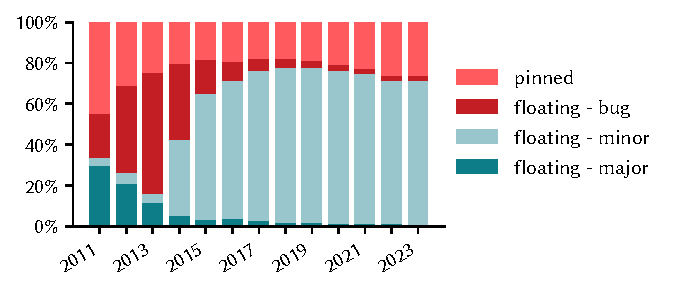
\includegraphics[width=\linewidth]{figs-pinning/versioning_trend_all.pdf}
        \caption{The distribution of version constraint types.}
        \label{fig:versioning}
    \end{subfigure}
    \begin{subfigure}[b]{0.46\linewidth}
        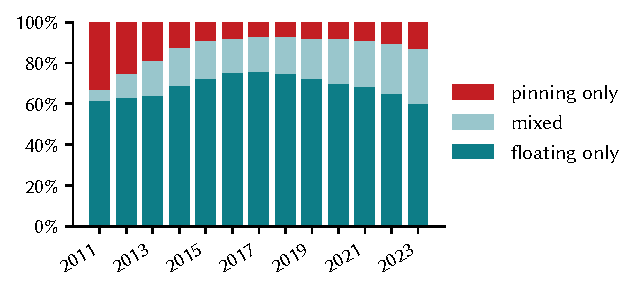
\includegraphics[width=\linewidth]{figs-pinning/versioning_strategy_trend_all.pdf}
        \caption{The distribution of project-level versioning strategies.}
        \label{fig:versioning-strategy}
    \end{subfigure}
    \caption{
    The distribution of version constraint types and project-level versioning strategies in each year in the dataset we use for answering RQ1 (see Section~\ref{sec:data-collection} for details) - we observe that after years of increasing floating adoption, since about 2020 the trend reverses with a shift toward pinning. In Figure~\ref{fig:versioning}, we ignore non-floating/pinning version constraints as they only occupy 0.83\% of version constraints in our dataset.
    }
    \label{fig:version-dist}
\end{figure}

Overall, controversies remain on whether the benefits of pinning outweigh its drawbacks, as manifested by online discussions~\cite{facts-vs-feelings, renovate-discussion, pinning-only-work} and evidenced by the contradicting results from the collected practitioner opinions in prior studies \cite{DBLP:journals/tse/JafariCAST22, DBLP:conf/sp/LadisaPMB23}.
However, to the best of our knowledge,  \textit{there is no quantitative evidence so far about the actual impact of pinning versus floating dependencies on the security and maintenance trade-offs in Table~\ref{tab:trade-offs}}.
To gather quantitative evidence about pinning and floating, we perform a repository mining study on the npm ecosystem, the most frequently discussed ecosystem in the literature.
Our study highlights an important complication that makes the discussion around pinning so difficult: Since a project can only control the version constraints of its direct dependencies, the actual impact of pinning as a local intervention is complicated and unclear, contingent upon both the decisions made upstream and the behaviors of dependency management tools. 
To measure this impact holistically from empirical data, we raise the following research question:
\begin{itemize}[leftmargin=20pt]
    \item \textbf{RQ1:} (\emph{Impact of Pinning}) How does the individual choice of pinning direct dependencies affect the overall security risks and maintenance costs in one's own dependency graph?
\end{itemize}
To answer this research question, we collect a large sample of npm packages and GitHub repositories using npm.
Then, we use an experimental time-traveling feature of the npm dependency resolver to simulate the evolution of their dependency graphs over a 12-month period.
We estimate the impact of pinning on a set of five security and maintenance-related metrics using \emph{fixed-effect panel regression}~\cite{bruderl2015fixed, hanck2021introduction}.
A key (and counter-intuitive) finding from our model is that for the purpose of reducing the attack surface of malicious updates, \textit{pinning is futile and can be even harmful} for projects with $\ge$498 direct and transitive dependencies (affecting 26\% of GitHub repositories in our dataset). That is, pinning is ineffective for one of its main goals, all while creating substantial costs for managing outdated, vulnerable, and conflicting dependencies. 

Inspired by this finding, we argue that \textit{ecosystem-level interventions} (e.g., investing resources to secure critical open-source projects) are more effective than the (possibly futile) local interventions of pinning direct dependencies to improve the overall resilience of an open-source ecosystem against malicious package updates.
To empirically test this hypothesis, we explore the second research question:
\begin{itemize}[leftmargin=20pt]
    \item \textbf{RQ2:} (\emph{Ecosystem-Level Interventions}) How effective is coordinating pinning among selected upstream packages in reducing the risk of malicious package updates ecosystem-wide? 
\end{itemize}
We answer this research question by simulating coordinated efforts in the entire npm dependency network.
We formulate attack models and defense strategies in the dependency network, define heuristics to intervene in selected upstream packages, and measure the overall risk of malicious package updates after the intervention.
Our findings indicate that it is possible to reduce the average spread of malicious package updates in the npm dependency network by nearly 30\% if we pin in 100 intentionally selected important packages.
However, as we will quantify, this intervention could be substantially more effective (up to 75\%) if npm implements a new \textit{transitive pinning} feature to allow packages to pass their entire pinned dependency graphs downstream.

\paragraph{Summary of Our Contributions} Our paper contributes novel quantitative evidence on the security and maintenance impact of version constraints in a packaging ecosystem, especially in light of recent concerns about malicious package updates.
Our findings align with the opinions of npm developers~\cite{DBLP:journals/tse/JafariCAST22} but contradict the views of security practitioners~\cite{DBLP:conf/sp/LadisaPMB23, DBLP:journals/ieeesp/ZahanKHSW23}, suggesting that pinning direct dependencies is futile (and can be even counter-productive) as protection against malicious package updates.
In addition, we contribute evidence that a new ecosystem-wide intervention, along with tooling changes and ecosystem-wide allocation of collectively pooled resources, can be an effective intervention against malicious package updates.
Our findings lead to concrete advice for developers and ecosystem policy makers to improve the state of software supply chain security (Section~\ref{sec:pinning-discussion}). 

\section{Background and Related Work}
\label{sec:background}

\paragraph{Dependency Management in npm}

\begin{figure}[b]
    \scriptsize
    \centering
\begin{minted}[
frame=lines,
framesep=2mm,
baselinestretch=1,
fontsize=\small,
escapeinside=()
]{json}
{ "name": "postcss-loader", "version": "7.3.3",
  "dependencies": {
    "webpack": ">=5.0.0"     (\textbf{\color{red}$\leftarrow$~\textsf{\textbf{floating - major}}})
    "cosmiconfig": "^8.3.5", (\textbf{\color{red}$\leftarrow$~\textsf{\textbf{floating - minor: $\ge$8.3.5, $<$9.0.0}}})
    "jiti": "~1.21.0",       (\textbf{\color{red}$\leftarrow$~\textsf{\textbf{floating - patch: $\ge$1.21.0, $<$1.22.0}}})
    "semver": "7.5.4"        (\textbf{\color{red}$\leftarrow$~\textsf{\textbf{pinned}}})
    "postcss": "^7.0.0 || ^8.0.1", (\textbf{\color{red}$\leftarrow$~\textsf{\textbf{other}}})
    "lodash": "git+ssh://git@github.com:lodash/lodash.git#v4.17", (\textbf{\color{red}$\leftarrow$~\textsf{\textbf{other}}})
  }, "devDependencies": {(...)}, (...) }
\end{minted}
\caption{
An example \Code{package.json} file. 
We modified version constraints in the original file to illustrate different types of version constraints defined in Section~\ref{sec:method-rq1}. Other details irrelevant to this paper are omitted.}
\label{fig:example-pkgjson}
\end{figure}

npm is the most widely used dependency manager for  JavaScript and TypeScript~\cite{npm}.
It consists of a package registry that hosts open-source components (called \emph{packages} in npm) and a command-line tool that helps projects reuse packages from the package registry.  
As of September 2024, the npm registry is the largest package registry, hosting more than 3 million packages and 25 million releases~\cite{module-counts}.
The npm command-line tool reads direct dependencies from a configuration file named \Code{package.json}.
%resolves all direct and indirect dependencies and their specific versions as a \emph{dependency graph}, and installs all the packages in the dependency graph to the local machine.
In the \Code{package.json} file (see Figure~\ref{fig:example-pkgjson} for an example), developers specify package names as the \emph{dependencies} of the project with a \emph{version constraint} for each dependency.
In addition, npm distinguishes different kinds of dependencies---usually, developers focus more on \emph{production dependencies}~\cite{DBLP:conf/kbse/LatendresseMCS22}, i.e., dependencies that will be included in the production build (for applications) or passed downstream (for packages), and are less concerned about security vulnerabilities if the dependencies are not used in production~\cite{DBLP:conf/esem/PashchenkoPPSM18, DBLP:conf/kbse/LatendresseMCS22}.

Given a \Code{package.json} file, npm will resolve a \textit{dependency graph} including not only dependencies specified in the \Code{package.json} file, but also all transitive dependencies required by dependencies.
The npm ecosystem is known as particularly fragmented with many tiny packages and high levels of reuse~\cite{DBLP:conf/sigsoft/AbdalkareemNWMS17, DBLP:journals/ese/DecanMG19}; a project commonly has orders of magnitude more transitive dependencies than direct ones~\cite{DBLP:journals/ese/DecanMG19}.
Dependency resolution can be complicated when multiple dependencies depend on the same third dependency but with conflicting version constraints; this is known as the \textit{diamond problem} or \textit{dependency hell} (see Figure~\ref{fig:rq2-example}). 
While it is highly problematic in other ecosystems~\cite{fan2020escaping,mancinelli2006managing,DBLP:conf/wcre/AbateCGZ20,DBLP:journals/tosem/BogartKHT21}, npm can install multiple distinct versions for the same package, but it will generally try to produce a dependency graph with fewer duplicate versions (i.e., deduplication~\cite{npm-install}). 
Optimal deduplication is NP-Complete~\cite{DBLP:conf/wcre/AbateCGZ20}, so npm uses a variety of heuristics to search for a ``good'' dependency graph satisfying all the version constraints while having fewer duplicate versions~\cite{npm-install}. 
%Attempts to resolve optimal dependency graphs using an SMT solver are ongoing~\cite{DBLP:conf/icse/PinckneyCGBCG23}. 

Importantly, \emph{dependency graphs are volatile}. 
Since npm always installs the latest version inside a floating versioning constraint, the same \Code{package.json} may result in different graphs as new package updates are released~\cite{DBLP:conf/icse/LiuCF00022}.
With floating, projects can keep dependencies up-to-date automatically, whereas developers often do not update pinned dependencies timely, even for those with known security vulnerabilities~\cite{DBLP:conf/icse/CoxBEV15, DBLP:journals/ese/KulaGOII18, DBLP:journals/tse/HeHZZ23}.

A key challenge to floating dependencies is \textit{breaking changes}: When an update changes expected behavior, the application can break without any action by its developer. Developers then need to react and either adapt their own code or downgrade the dependency~\cite{DBLP:journals/tosem/BogartKHT21}.
To control breaking changes, npm advocates for \emph{semantic versioning}~\cite{npm-semver}: A release should increment its major version number (e.g., from \Code{1.2.1} to \Code{2.0.0}) if it contains breaking changes, minor version number (e.g., from \Code{1.2.1} to \Code{1.3.0}) if it contains new features, and patch version number (e.g., from \Code{1.2.1} to \Code{1.2.2}) if it contains only bug fixes. If packages follow those conventions, automatic minor and patch updates should be safe. 
To support this practice, npm provides specific patterns to declare version ranges accepting minor (e.g., \Code{\^{}8.3.5}) and patch updates (e.g., \Code{\~{}1.21.0}); it also adopts floating versions for minor updates by default when a developer adds a dependency with  \Code{npm install}.
Although previous research has shown that 
%However, one important limitation of semantic versioning is that package developers need to decide whether their release contains breaking changes, which is a challenging open problem~\cite{DBLP:conf/oopsla/LamDP20}.
%also covered by Hyrum's Law: \textit{``with a sufficient number of users of an API, it does not matter what you promise in the contract: all observable behaviors of your system will be depended on by somebody''}~\cite{hyrum-law}.
packages may fail to obey semantic versioning~\cite{DBLP:journals/jss/RaemaekersDV17, semantic-versioning-sucks, DBLP:conf/kbse/ZhangLXCF0022, DBLP:conf/issta/JayasuriyaT0OB23} and developers may turn to pinning instead if they have lost trust in its reliability~\cite{stop-version-range, semantic-versioning-sucks},
 semantic-versioning-based floating is still widely accepted and used by npm developers~\cite{DBLP:conf/msr/0001PSTB19, DBLP:journals/tse/DecanM21, DBLP:conf/msr/PinckneyCGB23, DBLP:journals/tse/JafariCAST22}.
In fact, without discussion of supply chain attacks, the survey by~\citet{DBLP:journals/tse/JafariCAST22} shows that npm developers generally consider pinned dependencies as a ``smell,'' indicating a compromise that will accumulate technical debt and bring negative consequences in the long term.

Finally, it is worth noting that the above discussion applies not only to floating direct dependencies but also to floating transitive dependencies even if the developer pins all their direct dependencies.
Developers usually have no control over how their dependencies float or pin transitive dependencies.
As a workaround, npm (as many other ecosystems) provides functionality to \textit{freeze} and store a project's entire dependency graph with a lock file (\Code{package-lock.json}~\cite{npmpkglock}). % storing the entire resolved dependency graph. 
A lock file ensures the reproducibility of npm builds, but
it has two limitations: (1)~it is restricted to applications (the root of the dependency graph) whereas components used as dependencies cannot pass their lock decisions to downstream applications; it is hence not very useful for packages; (2)~it is not designed (hence very difficult) to be manually maintained, so floating version constraints in \Code{package.json} will still cause automatic updates every time a lock file is generated.

\paragraph{Software Supply Chain Security}

The term \textit{software supply chain} is an umbrella term referring to all the software components, processes, and tools that a software project relies on~\cite{software-supply-chain-guide}.
For a project using npm, all packages in its dependency graph are part of its supply chain.
Most software projects nowadays are built upon a collaboratively developed open-source software supply chain~\cite{eghbal2016roads}; the 3~million packages in the npm package registry are a prominent example.

Software supply chains are fragile.
Such fragility comes from the collaborative and distributed nature of open-source development: Projects are often built with a large number of open-source components, each of them maintained by different groups of developers~\cite{schueller2024modeling}.
Meanwhile, popular components are directly or transitively used by a large number of downstream applications.
Consequently, any single weakness in the software supply chain could have a huge impact on the entire ecosystem~\cite{DBLP:journals/ese/DecanMG19, DBLP:conf/uss/ZimmermannSTP19}, creating a large attack vector for malicious actors and making the software industry increasingly concerned with software supply chain security~\cite{DBLP:journals/usenix-login/GeerTM20,DBLP:conf/sp/LadisaPMB23}.

In recent years, a significant amount of practitioner attention has been drawn to the rising threat of \emph{software supply chain attacks}~\cite{DBLP:conf/dimva/OhmPS020, DBLP:conf/sp/LadisaPMB23}. 
Although the attackers may attempt to trick malware installation in other ways (e.g., typosquatting~\cite{DBLP:conf/eurosp/VuPMPS20}), the most concerning incidents of software supply chain attacks are \emph{malicious package updates}, in which malicious actors \textit{intentionally} compromise an open-source component to inject malware into its (often many) downstream dependents.
While not every security vulnerability is exploitable in practice (leading developers to treat them as false positives)~\cite{DBLP:conf/codaspy/YounisMAR16, DBLP:journals/corr/abs-1908-04856, mirhosseini2017can}, malicious package updates can immediately harm the infected downstream dependents~\cite{martinez2021software}. 
They may also be well obfuscated and often very difficult to detect~\cite{xz-utils}.
Their high catastrophic potential and lack of controllability amplify the signal of real incidents and elevate public risk perception (e.g., in a way similar to nuclear hazards~\cite{slovic1987perception}).
As a result, malicious package updates are considered one of the primary threats in today's threat landscape~\cite{enisa-report, whitehouse-order}.
 
As our previous discussion of the pinning versus floating debate illustrates, many dependency management practices have security implications and involve trade-offs between conflicting priorities~\cite{DBLP:conf/ccs/PashchenkoVM20}.
Previous studies have investigated various practices, such as dependency adoption, updates, abandonment, migration, and the use of dependency management tools~\cite[e.g.,][]{DBLP:journals/ese/KulaGOII18, DBLP:conf/sigsoft/VargasATBG20, DBLP:conf/sigsoft/HeHGZ21, DBLP:conf/sigsoft/MillerKV23, DBLP:journals/tse/HeHZZ23}.
%and reproducible builds~\cite{DBLP:conf/sp/FourneWEFA23}. 
It is worth noting, however, that most prior research in the software engineering community is centered around the mitigation of security vulnerabilities.
%less attention has been paid to \textit{practices that may defend against the rising threat of software supply chain attacks.}
%Researchers have also conducted qualitative studies to inquire practitioner opinions on certain practices~\cite{DBLP:conf/ccs/PashchenkoVM20, DBLP:conf/sp/FourneWEFA23, DBLP:conf/sp/WermkeKWSRAF23}.
%In support of floating, researchers have revealed how floating may help, and how pinning may block, the propagation of security fixes in packages~\cite{DBLP:journals/ese/ChinthanetKMIIM21, DBLP:journals/tse/0038SP00C0023}. 
%On the other hand, security practitioners argue that pinning is necessary for applications to defend against supply chain attacks, and security vulnerabilities should be handled by manual updates with careful reviews.
On the other hand, the security community has recently consolidated best practices to defend against supply chain attacks, such as the OpenSSF Scorecard project~\cite{DBLP:journals/ieeesp/ZahanKHSW23} and the survey by \citet{DBLP:conf/sp/LadisaPMB23} introduced in Section~\ref{sec:pinning-introduction}.
However, these (supposed) security best practices may interact with existing \emph{software engineering} trade-offs, among which the pinning versus floating problem is particularly complicated (Table~\ref{tab:trade-offs});  the strongly held convictions from both sides lead to a considerable amount of controversy among practitioners~\cite{facts-vs-feelings, renovate-discussion, pinning-only-work}.

\paragraph{Novelty of Our Research.} 
There have been many prior studies on the use of version constraints~\cite{DBLP:conf/msr/0001PSTB19, DBLP:journals/tse/DecanM21, DBLP:conf/msr/PinckneyCGB23, DBLP:conf/sp/LadisaPMB23} and the trade-offs  around semantic versioning with regards to maintenance effort, breaking changes, and security vulnerabilities~\cite{DBLP:journals/tse/JafariCAST22, DBLP:journals/tosem/BogartKHT21,DBLP:journals/jss/RaemaekersDV17}.
However, the new threat of \textit{malicious package updates} complicates the previously discussed trade-offs, as \emph{malicious actors intentionally break semantic versioning}, often disguising their attacks as patch releases for maximum propagation~\cite{node-ipc}.
The changed threat landscape and the complexity of this pinning versus floating problem eventually lead to controversies and divergence in practitioner opinions~\cite{facts-vs-feelings, renovate-discussion, pinning-only-work, DBLP:conf/sp/LadisaPMB23, DBLP:journals/tse/JafariCAST22}.
Prior studies are either collecting these opinions~\cite{DBLP:journals/tosem/BogartKHT21, DBLP:journals/tse/JafariCAST22, DBLP:conf/sp/LadisaPMB23} or aggregating descriptive statistics from software repositories~\cite{DBLP:conf/msr/0001PSTB19, DBLP:conf/msr/PinckneyCGB23, DBLP:journals/tse/DecanM21, DBLP:journals/jss/RaemaekersDV17}; we are not aware of any prior study that attempted to quantify the impact of version constraints using statistical modeling methods.
To shed light on resolving the controversy, we believe it is vital to conduct data-driven research and quantitatively measure the actual impact of version constraints while taking all the previously discussed trade-offs into consideration (Table~\ref{tab:trade-offs}).
This forms the main motivation of our study.

\section{RQ1: How does the individual choice of pinning direct dependencies affect the overall security risks and maintenance costs in one's own dependency graph?}

As we discussed above, dependency pinning is often acknowledged as a security best practice to reduce the attack surface for malicious package updates~\cite{DBLP:conf/sp/LadisaPMB23, DBLP:journals/ieeesp/ZahanKHSW23}, but controversies remain on whether the security benefits of pinning outweigh its maintenance drawbacks~\cite{facts-vs-feelings, renovate-discussion, pinning-only-work, DBLP:conf/sp/LadisaPMB23, DBLP:journals/tse/JafariCAST22}.
Importantly, a project only has control over the version constraints of its direct dependencies, but the impact of pinning direct dependencies is complicated and unclear, contingent upon upstream practices and dependency management tools.
Hence, the goal of RQ1 is to empirically measure the actual security and maintenance impact of this intervention (i.e., pinning direct dependencies).

\subsection{Data Collection}
\label{sec:data-collection}

We aim to build a balanced dataset of packages (e.g., libraries, frameworks) and applications (e.g., websites, tools), as both need to manage dependencies but may differ in important ways.
Thus, we use two data sources: (1) \emph{npm packages}, (2) \emph{GitHub repositories using npm} that are not npm packages.
Note that neither data source is a clear representation of libraries or applications. 
Some npm packages may be applications, and some GitHub repositories may be libraries that have not been uploaded to the npm registry. 
Still, combining the two should produce a stratified sample including both the representation of libraries and applications in the wild.


For the first data source, npm packages, we curate a large dataset of popular and non-obsolete npm packages. We avoid focusing only on the few most popular packages, as they are not necessarily representative of common development practices in npm (they tend to occupy an upstream position with no dependencies or a very small dependency graph). 
We use the following data collection process:
First, we use npm-follower~\cite{DBLP:conf/sigsoft/PinckneyCG023} (September 2023 dump) to obtain a complete list of npm packages and releases at that time.
Then, we collect year-long download statistics as a popularity measure (between September 06, 2022, and September 05, 2023) using the npm API. For each package, we also identify its corresponding GitHub repository from npm metadata.
Next, using this dataset, we select the top 5\% most downloaded packages (21,218+ downloads) that have links to a GitHub repository and discard the bottom 25\% of these packages with the lowest number of stars and issues in GitHub (specifically, less than 10 stars and 8 issues), to ensure that the remaining are actively maintained open-source packages.
To further ensure they are not obsolete, we discard packages that have no release in the last two years at the time of the dataset cutoff (September 2023).
We discard packages without any production dependencies in the latest release and end up with 41,516 npm packages.

For the second data source, we curate a dataset of GitHub repositories using npm, but are not npm packages, from World of Code~\cite{DBLP:journals/ese/MaDBAVTKZM21} (version V).
First, we select the JavaScript and TypeScript projects with top 1\% stars (i.e., \# stars $\ge$ 14) as a rough popularity threshold from its deduplicated GitHub metadata~\cite{DBLP:conf/msr/SpinellisKM20}.
To filter out small (and likely toy) projects, we discard projects with the bottom 25\% of commits and active months (specifically, $\le$84 commits and $\le$13 active months).
Then, we filter out projects that have been inactive (no commit) in the last two years at the time of dataset cutoff (September 2023).
To find GitHub repositories using npm, we retain projects with a \Code{package.json} file in their root folder. 
Finally, we discard repositories without any production dependencies and repositories whose \Code{name} field in \Code{package.json} matches a package name in npm---thus removing the ones more likely to be npm packages themselves.
This results in a total of 12,197 GitHub repositories.

As the two data sources are heavily imbalanced and the simulations (see Section~\ref{sec:method-rq1}) are computationally expensive, we downsample the two data sources to 10,000 npm packages and 10,000 GitHub repositories, respectively (uniform random sampling each).
We chose 10,000 each because it is computationally feasible for our simulation (in our case, two weeks of computation) and offers very high statistical generalizability.
In the remainder of RQ1, we will refer to the 10,000 npm \textit{packages} and the 10,000 GitHub \textit{repositories} collectively as \emph{projects}.

\begin{table}[t]
    \scriptsize
    \centering
    \caption{Descriptive statistics of the studied npm packages and GitHub repositories (excluding npm packages). The number of transitive dependencies is an estimate using successful dependency resolutions (Section~\ref{sec:method-rq1}).}
    \begin{tabular}{lrrrrrrrr}
      \toprule
         & \multicolumn{4}{c}{\textbf{npm packages}} & \multicolumn{4}{c}{\textbf{GitHub repositories (excl. npm packages)}} \\
         & Min & Median & Mean & Max & Min & Median & Mean & Max\\
      \midrule
       \# Annual Downloads    & 21,234  & 234K & 24.7M & 516M & \multicolumn{4}{c}{N/A}\\ 
       \# Stars         & 8 & 345 & 6,431.80 &  220K & 14 & 62 & 694.72 & 330K\\
       \# Issues        & 10 & 569 & 6338.55  & 87,258 & 0 & 101 & 652.62 & 75,561\\
       \# Commits       & 1 & 1,728 & 30,064.11 & 10.1M & 84 & 632 & 6215.72 & 7.17M\\
       \# Active Months & 1 & 48 & 60.7 & 324 & 13 & 36 & 44.26 & 323\\ 
       \# Direct Dependencies (Production)  & 1 & 3 & 5.78 & 283 & 1 & 11 & 16.83 & 492 \\
       \# Direct Dependencies (All) & 1 & 10 & 14.58 & 283 & 1 & 23 & 32.03 & 502 \\
       \# Transitive Dependencies (Production) & 0 & 11 & 65.55 & 2,320 & 0 & 150 & 391.51 & 3,722\\
       \# Transitive Dependencies (All) & 0 & 253 & 414.74 & 3,141 & 0 & 848 & 893.18 & 4,013\\
      \bottomrule
    \end{tabular}
    \label{tab:dataset}
\end{table}

\paragraph{Dataset Overview.}
We summarize the descriptive statistics from both data sources in Table~\ref{tab:dataset}.
Most of the projects in our dataset are popular and active.
As expected, GitHub repositories tend to have a much larger dependency graph than npm packages.
A median GitHub project has 11 direct dependencies and 150 transitive dependencies in production (23 direct and 848 transitive if we include development dependencies).
This confirms our intuition that many projects have orders of magnitude higher numbers of transitive dependencies compared with direct ones. 

In Figure~\ref{fig:version-dist}, we provide an overview of the use of version constraints in our dataset,
which largely mirrors findings of prior studies~\cite{DBLP:conf/msr/0001PSTB19, DBLP:journals/tse/DecanM21, DBLP:conf/msr/PinckneyCGB23}, but shows a previously not observed change in trend in more recent data, where developers start to pin more dependencies since around 2020.
Specifically, we aggregate dependency declarations of each project in each year, looking back at past revisions (releases for npm packages and commits for GitHub repositories).  
To reduce noise introduced by projects with a massive number of revisions, we sample one revision for each project in each year, as also commonly done in prior studies~\cite[e.g.,][]{DBLP:conf/msr/PinckneyCGB23, DBLP:conf/kbse/XuHGZ23}.
For each revision, we parse the version constraints of all its production dependencies in its \Code{package.json} file, according to the npm semver syntax~\cite{npm-semver}, and categorize the version constraints into five different types: (1) \emph{floating - major}, (2) \emph{floating - minor}, (3) \emph{floating - patch}, (4) \emph{pinned}, and (5) \emph{other}. 
Examples of these different version constraint categories can be found in Figure~\ref{fig:example-pkgjson}.
Overall, we find that semantic-versioning-based floating is used the most in the npm ecosystem but  pinning is still the second most popular choice, with a rising popularity since around 2020, even though npm does not advocate pinning~\cite{npm-semver}.
This aligns with our intuition that the rising concern of malicious package updates triggers changes in practitioner practices.
\begin{comment}
Overall, semantic-versioning-based floating is the majority in the npm ecosystem, but pinning is still the second most popular choice even if npm does not advocate pinning~\cite{npm-semver}.
In the parsed dependency declarations, 71.83\% are \emph{floating - minor}, 21.71\% are \emph{pinned}, 3.99\% are \emph{floating - bug}, 1.64\% are \emph{floating - major}, and 0.83\% are \emph{other}.
We also see a rise of \emph{floating - minor} and the fall of both \emph{floating - bug} and \emph{pinned} before 2018, but its popularity decreases afterward, replaced by a resurgence of pinning (Figure~\ref{fig:versioning}).
The decline of \emph{floating - bug} in Figure~\ref{fig:versioning} can be attributed to the npm default change in 2014~\cite{npm-default-change} from \emph{floating - bug} to \emph{floating - minor}, which was an effort of npm to explicitly commit to semantic versioning.
Additionally, we believe the decline of \emph{pinning} before 2018 can be attributed to growing optimism toward semantic versioning and automated dependency updates. 
However, the resurgence of pinning since 2018 indicates that an increasing number of developers have encountered issues with floating and started to use pinning instead, as also indicated in the grey literature~\cite{floating-discussion,
stop-version-range, pin-exact-dep-versions, pin-your-npm-yarn-dependencies}.
This trend might have also been further boosted by the recognition of pinning as a security best practice~\cite{DBLP:conf/sp/LadisaPMB23, DBLP:journals/ieeesp/ZahanKHSW23}.
The distributions of version constraints in our data (Figure~\ref{fig:versioning}) generally align with findings from past studies~\cite{DBLP:conf/msr/0001PSTB19, DBLP:journals/tse/DecanM21, DBLP:conf/msr/PinckneyCGB23}, but our analysis with more recent data and disaggregated by active projects in each year shows the increasing popularity of pinning since 2018, which was not previously reported.
\end{comment}
To further inform our study design, we examine how individual projects demonstrate preferences for pinning or floating (Figure~\ref{fig:versioning-strategy}).
We categorize a project's overall versioning strategy into \emph{floating only}, \emph{pinning only}, or \emph{mixed} based on the version constraints of its production dependencies.
%To this end, we categorize a project's overall versioning strategy into one of the following based on the version constraints of its production dependencies:
%(1) \textbf{\emph{floating only}}: All of its dependency declarations are \emph{floating - major},  \emph{floating - minor},  \emph{floating - bug}, or \emph{other} and none of the dependency declarations are \Code{pinned}; 
%(2) \textbf{\emph{pinning only}}:  All of its dependency declarations are \emph{pinned} or \emph{other} and none of the dependency declarations are \emph{floating}; 
%(3) \textbf{\emph{mixed}}: Some of its dependency declarations are \emph{pinned} and some of its version constraints are \emph{floating}.
%We compute the overall distribution of versioning strategies for all the sampled releases/commits in each year and plot its longitudinal evolution in stacked bar charts. 
%We find that 68.86\% of the projects use a \emph{floating only} strategy, 21.91\% use a \emph{mixed} strategy, and 9.23\% use a \emph{pinning only} strategy.
%Even if we only look at the projects with at least five direct dependencies, 54.67\% use a \emph{floating only} strategy, and 7.07\% use a \emph{pinning only} strategy.
Similar to the trend of version constraints, the popularity of \emph{floating only} strategy increased from 2011 to 2018 but has fallen since then, replaced by more adoption of \emph{pinning only} and \emph{mixed} strategy in the last five years.
Our results indicate that although projects sometimes make deliberate decisions per dependency~\cite{DBLP:journals/tosem/JafariCSA23}, the majority of projects make a uniform decision, motivating us to use similar alternations in our simulations (Section~\ref{sec:method-rq1}).

\subsection{Method}
\label{sec:method-rq1}

\paragraph{Overview}
At a high level, we take a \emph{counterfactual analysis} approach~\cite{morgan2015counterfactuals}---that is, estimating the causal effect of pinning by comparing the ``what-if'' differences with not pinning in each project.
This leads to our design of comparing metrics %(one for each of the five trade-offs commonly raised in favor or against pinning, previously summarized in Table~\ref{tab:trade-offs}), 
between a \emph{control} condition consisting of our observed projects, and a (simulated) \emph{treatment} condition wherein we alter each of the project's \Code{package.json} to pin all its direct dependencies.
We design a set of five outcome metrics in the project dependency graph to measure the five trade-offs raised in favor or against pinning, previously summarized in Table~\ref{tab:trade-offs}.
However, the comparison of these metrics is challenging as we would need to simulate how pinning would change the dependency graph of a focal project.
What's more, the values of metrics may change over time as the focal project and the ecosystem continuously evolves.
To overcome the first challenge, we leverage a hack in the npm dependency resolver for accurate time-traveling dependency resolution~\cite{DBLP:conf/msr/PinckneyCGB23}.
To overcome the second challenge, we organize the simulated data into \textit{balanced panels}, wherein each project is observed and simulated at five different times under both conditions (control and treatment). 
Then, we use \emph{fixed-effects panel regression} to estimate the effect of pinning 
separately for each of the five outcome metrics. 
Panel regression is a statistically sound econometric technique to model double-dimensional data (data collected from multiple units across different time periods) robustly to unobserved heterogeneity (i.e., project/time-specific characteristics that affect the outcome metric but are not directly measured or included in the model)~\cite{bruderl2015fixed, hanck2021introduction}.
Next, we give more details on the simulation setup and regression analysis.

\paragraph{Simulation Setup}
To implement the above design, we get the latest revision between September 2021 and September 2022 for each project in our dataset.
Then, we use September 12, 2022 as a starting time point for simulations (denoted $t_0$). 
We recreate the state of each project at this timestamp $t_0$, including the \Code{package.json} files, and resolve the corresponding dependency graphs (denoted as $G_{t0}$). 
Such historical resolution is non-trivial as we will need to reconstruct the state of the npm ecosystem at those times. 
Fortunately, thanks to a previous report by \citet{DBLP:conf/msr/PinckneyCGB23}, we use the undocumented \Code{\,-{}-before\,} argument in the npm command-line tool to enable \textit{time-traveling} dependency resolution.
Next, we create an altered version of each \Code{package.json} file by removing the ``caret'' and ``tilde'', i.e., pinning all direct dependencies to the minimal version specified in \Code{package.json}, and resolve the simulated dependency graph ($G'_{t0}$) analogously. 
This step results in two observations for each project, that feed into our ``control'' and ``treatment'' groups, respectively.
Similarly, we check out four additional versions of the \Code{package.json} file, at four evenly-spaced fixed 90-day intervals from December 11, 2022 to September 7, 2023 (denoted $t_1 \ldots t_4$). At each time point, we resolve the corresponding original and simulated (all-pinning) dependency graphs, which adds four additional observations per project into each of our ``control''  and ``treatment'' groups.
Note that for each project and treatment condition, we intentionally resolve dependency graphs at different time points from the same \Code{package.json} file; this setting, combined with our outcome metrics below, provides a framework to estimate the costs of action (or risks of not taking action) over the observation period, independent of the actual project actions taken during that period.

\paragraph{Outcome Metrics}
For each of the five original and simulated dependency graphs resolved for a given project, we compute five security- and maintenance-related metrics, each corresponding to one dimension of trade-offs in Table~\ref{tab:trade-offs}.
Their definitions are as follows:
\begin{enumerate}[leftmargin=20pt]
    \item \textsf{\# of floating dependencies} (\Code{n\_floating}):  The number of edges in the dependency graph with a floating version constraint. This metric captures \textit{attack surface}, i.e., the number of packages where a malicious update would be installed automatically if they were attacked.
    \item \textsf{\# of automatic updates} (\Code{n\_auto\_updates}):  The number of automatic updates happened between $t_0$ and $t$ for the dependency graph at time $t$. This metric captures the risk of \emph{breaking changes}, assuming that breaking changes happen uniformly randomly among new releases.
    \item \textsf{\# of security vulnerabilities} (\Code{n\_vuln}): The number of known vulnerable dependencies in the dependency graph based on entries in GitHub Advisory~\cite{github-adv} at time $t$. This metric captures the maintenance cost introduced by the need to remove \emph{security vulnerabilities} in the project (usually by manually updating to a newer version). 
    \item \textsf{\# of outdated dependencies} (\Code{n\_outdated\_deps}):  The number of outdated direct dependencies in the dependency graph is based on whether a newer release exists at time $t$. This metric captures the maintenance cost introduced by the need to manually update \emph{outdated dependencies}. 
    \item \textsf{\# of bloated dependencies} (\Code{n\_bloated}):   The number of packages with more than one version simultaneously present in the dependency graph (i.e., bloated). This metric captures the maintenance cost introduced by \emph{dependency conflicts} because npm resolves such conflicts by allowing different versions of the same package at different levels~\cite{how-npm3-works}.
\end{enumerate}
Intuitively,  \Code{n\_floating} and \Code{n\_auto\_updates} should decrease with pinning and increase with floating;
\Code{n\_vuln}, \Code{n\_outdated\_deps} and \Code{n\_bloated} should decrease with floating and increase with pinning. We designed all metrics such that lower values are generally better (e.g., lower costs or risk).

\paragraph{Panel Regression}
%\emph{Panel Regression}
For each metric $M$, we fit the following panel regression model: %
\begin{equation}
\label{eq:plm}
\ln(M+1) \sim \text{\emph{pinning}} + \ln(size(G)) + \text{\emph{pinning}} \times \ln(size(G)) + \alpha + \beta 
\end{equation}
In this model specification, $\alpha$ and $\beta$ represent project-fixed and time-fixed effects, respectively. 
These two variables give the model robustness to unobserved heterogeneity, allowing us to model the unmeasured project-specific or time-specific characteristics that might affect the dependent variable.
The main variable of interest is the \textit{pinning} flag, whose estimated coefficient, if statistically significantly different from zero, represents the average change in metric $M$ relative to the default ``control'' condition, while holding fixed the other factors.
Finally, we model an explicit interaction with the size of the dependency graph $size(G)$ (i.e., number of nodes), to test whether the effect of pinning varies with $size(G)$---one can expect, e.g., that having more direct and transitive dependencies increases the attack surface of a downstream project.
The models are fitted using the R \Code{plm} package~\cite{r-plm}.

\paragraph{Limitations and Threats to Validity}

Our model design should allow reliable estimates of the impact of pinning, but it relies on accurate dependency resolution at past points in time.
While we believe that our solution is accurate, simulations can still deviate from the realities in the past due to npm behavior changes, configuration differences, etc. 
The dependency resolution attempts may also fail with an error, upon which we discard the data point: In total, we have a success ratio of 83.6\% for npm packages and 87.7\% for GitHub repositories.
For the failed resolutions, npm's error logs indicate the failures can be due to \emph{bad version constraints} (41.9\%), \emph{missing packages} (37.0\%), \emph{git errors} (8.9\%), \emph{bad URLs} (5.7\%), \emph{missing local files} (2.6\%), \emph{incompatible OS} (2.4\%), and others.
Resolution failures can happen for many reasons, such as a release being taken down by npm and a project depending on a package not present in the npm registry (i.e., likely proprietary).
As such software builds are inherently volatile~\cite{DBLP:conf/icse/SeoSEAB14, DBLP:conf/icse/DmeiriTWBLDVR19}, we believe these errors are difficult, if not impossible, to fix in an automated simulation pipeline.
Thus, we conclude that the success ratio is acceptable and the scale of our data is sufficient for our study design, being comparable with or larger than datasets in the medical and econometrics literature where similar designs are adopted (e.g.,~\cite{crouse1999randomized, stutzer2006does, gerstorf2010late}).

\setlength{\abovecaptionskip}{2pt}%
\setlength{\intextsep}{0pt}
\begin{wrapfigure}{r}{0.35\textwidth}
    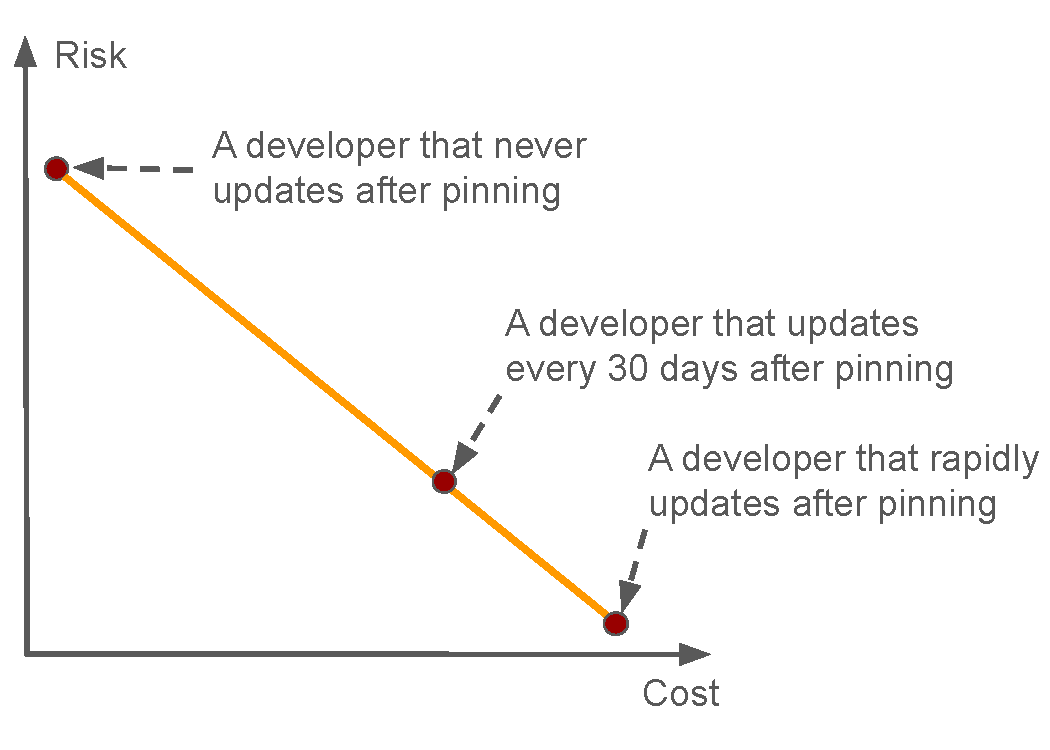
\includegraphics[width=\linewidth]{figs-pinning/tradeoff-pinning.pdf}
    \caption{An illustration of the trade-off between cost and risk after pinning.}
    \label{fig:tradeoff-pinning}
\end{wrapfigure}
\setlength{\abovecaptionskip}{10pt}

Our simulation setup enables a holistic approach to measure the costs of taking action (or the risks of not), but does not fully take into account the complexity of project actions that may happen over a year.
For example, a project that opts for pinning can invest no effort in updating its pinned dependencies, rapidly update upon every new release of a dependency, or take an intermediate approach (e.g., update every 30 days).
In other words, for at least some of our outcome metrics (e.g., security vulnerabilities), developers using a pinning strategy can choose how much effort to invest in manual actions to further trade-off costs and risks (Figure~\ref{fig:tradeoff-pinning}).
In this paper, all outcome metrics are estimated from the conservative case of no manual developer actions; we leave the exploration of other cases to future work.

In terms of the metric design, we implicitly assume that malicious package updates and breaking changes follow a uniform random distribution, counting potential rather than actual events.
For malicious package updates, real attackers are generally opportunistic, and existing research does not show any noticeable statistical patterns in attack target selection~\cite{DBLP:conf/dimva/OhmPS020, DBLP:conf/sp/LadisaPMB23}.
Thus, we believe it is reasonable to assume attacks to happen uniformly randomly among packages.
For breaking changes, it could be possible to get more accurate estimations from static analysis or regression testing, but adopting either would severely limit and bias the amount of data available for modeling purposes.
Specifically, (1) static analysis only works well on TypeScript packages, (2) regression testing is only applicable to projects with a running test suite and prior regression testing studies collected at most a few hundred JavaScript projects with breaking changes~\cite{DBLP:conf/ecoop/MezzettiMT18, kong2024towards}.
In fact, we believe that breaking changes are so hard to avoid---even in well-managed projects (see Hyrum's Law~\cite{hyrum-law})---and well-tolerated in the npm ecosystem~\cite{DBLP:journals/tosem/BogartKHT21} that the uniformly random assumption is actually a reasonable approximation to quantify the expected risk (or cost) of breaking changes on a large scale npm based dataset.

In terms of external validity, it is important to note that our study are specific to the npm ecosystem and the results may not generalize to other ecosystems that adopt different baseline practices.
For example, the Maven ecosystem (Java) is smaller~\cite{module-counts}, conducts pinning extensively~\cite{DBLP:conf/msr/0001PSTB19}, and handles dependency conflicts differently~\cite{DBLP:conf/sigsoft/WangWLWWYYZC18}, so the trade-off between pinning and floating could manifest in a different manner.
In addition, generalizations to closed-source applications should also be careful as they may have different characteristics compared with our dataset. %(e.g., some sources suggest that they have more dependencies and larger dependency graphs~\cite{sonatype-report}).


\subsection{Results}
\label{sec:results-rq2}

In this section, we report results based on \emph{production dependency graphs} (i.e., excluding development dependencies) from all projects in all time points (Table~\ref{tab:pinning-regression}).
Wald tests show that the full model (with pinning and the interaction) is preferable for all five outcome variables ($p<0.001$) compared to a null model with only $size(G)$ as an independent variable.
Note while development dependencies are generally considered irrelevant for security vulnerabilities~\cite{DBLP:conf/kbse/LatendresseMCS22, DBLP:conf/esem/PashchenkoPPSM18}, they form an important attack surface for malicious package updates that compromise build systems~\cite{DBLP:conf/sp/LadisaPMB23, DBLP:conf/dimva/OhmPS020}.
Therefore, we have also explored the robustness of our findings: (1) in dependency graphs with development dependencies, (2) separately on npm packages and GitHub repositories, and (3) using only data collected at $t_0$. 
The results are highly consistent and available in the replication package (Section~
\ref{sec:data-availability}).

\begin{table}
    \footnotesize
    \renewcommand{\arraystretch}{1.2}
    \centering
    \caption{The descriptive statistics (aggregated over all time points) and the longitudinal evolution of the studied security and maintenance related metrics between the control and treatment group (pinning).
    }
    \begin{tabular}{llrrrrrrc}
    \toprule
        Metric & Condition & Min & 25\% & Median & 75\% & Max & Mean & Evolution  \\
    \midrule
       \texttt{n\_floating} & 
\includegraphics[height=1.5mm]{figs-pinning/legend_control.png} Control & 0 & 8 & 65 & 335 &  9,191 & 432.35 &\multirow{2}{*}{\adjustimage{height=10mm,valign=m}{figs-pinning/n_floating_all.pdf}} \\
       & 
\includegraphics[height=1.5mm]{figs-pinning/legend_pinning.png} Pinning & 0 & 5 & 60 & 327 & 8,909 & 427.83 & \\\addlinespace
       \texttt{n\_auto\_updates} & 
\includegraphics[height=1.5mm]{figs-pinning/legend_control.png} Control  & 0 & 0 & 3 & 21 & 1,354 & 30.30 & \multirow{2}{*}{\adjustimage{height=10mm,valign=m}{figs-pinning/n_auto_updates_all.pdf}}\\
       & 
\includegraphics[height=1.5mm]{figs-pinning/legend_pinning.png} Pinning & 0 & 0 & 2 & 14 & 662 & 24.86  \\\addlinespace
       \texttt{n\_vuln} & 
\includegraphics[height=1.5mm]{figs-pinning/legend_control.png} Control & 0 & 0 & 0 & 2 & 85 & 2.13  & \multirow{2}{*}{\adjustimage{height=10mm,valign=m}{figs-pinning/n_vuln_all.pdf}} \\
       & 
\includegraphics[height=1.5mm]{figs-pinning/legend_pinning.png} Pinning & 0 & 0 & 0 & 2& 97&  2.70  \\\addlinespace
       \texttt{n\_outdated\_deps} & 
\includegraphics[height=1.5mm]{figs-pinning/legend_control.png} Control & 0 & 1 & 2 & 7 & 225 & 5.96  & \multirow{2}{*}{\adjustimage{height=10mm,valign=m}{figs-pinning/n_outdated_deps_all.pdf}} \\
       & 
\includegraphics[height=1.5mm]{figs-pinning/legend_pinning.png} Pinning & 0 & 1 & 4 & 11 & 302 & 8.78  \\\addlinespace
       \texttt{n\_bloated} & 
\includegraphics[height=1.5mm]{figs-pinning/legend_control.png} Control & 0 & 0 & 1 & 13 & 650 &  22.38  & \multirow{2}{*}{\adjustimage{height=10mm,valign=m}{figs-pinning/n_bloated_all.pdf}}  \\
       & 
\includegraphics[height=1.5mm]{figs-pinning/legend_pinning.png} Pinning & 0 & 0 & 1 & 15& 639 & 23.51  \\\addlinespace
    \bottomrule
    \end{tabular}
    \label{tab:metric-values}
    \renewcommand{\arraystretch}{1}
\end{table}

\begin{table}
\footnotesize
\centering 
\caption{The fixed-effect panel regression results. 
We obtain a high goodness-of-fit for \texttt{n\_floating} (R$^{2}$$\ge$0.6), acceptable goodness-of-fit for \texttt{n\_vuln}, \texttt{n\_outdated\_deps}, and \texttt{n\_bloated} (R$^{2}$$\ge$0.1), and low goodness-of-fit for \texttt{n\_auto\_updates} (R$^{2}$$<$0.1).
The R$^{2}$ values are comparable with similar prior studies~\cite[see, e.g.,][]{DBLP:conf/sigsoft/ValievVH18, DBLP:conf/icse/ZahanSHW23}. 
Note that since our goal is explanatory (not predictive), we do not evaluate models based on on R$^{2}$ values, but conduct a series of robustness checks to see whether the findings are robust over different settings (Section~\ref{sec:results-rq2}).
We report local effect sizes computed using Cohen's $f^2$~\cite{selya2012practical}.
}
\label{tab:pinning-regression} 
\begin{tabular}{lrrrrr} 
  \toprule
   & \multicolumn{5}{c}{$\ln($\emph{Dependent Variable}$) + 1$} \\ 
   & \texttt{n\_floating} & \texttt{n\_auto\_updates} & \texttt{n\_vuln} & \texttt{n\_outdated\_deps} & \texttt{n\_bloated}\\
  \midrule
  \emph{pinning} & $-$0.519$^{***}_{+++}$ & $-$0.274$^{***}_{+}$ & 0.011$^{***}_{+}$ & 0.302$^{***}_{+++}$ & 0.029$^{***}_{+}$\\ 
   & (0.006) & (0.005) & (0.005) & (0.005) & (0.003)\\ \addlinespace
  $\ln(size(G))$ & 1.084$^{***}_{+++}$ & 0.794$^{***}_{+}$ & 0.283$^{***}_{+}$ & 0.068$^{***}$ & 0.631$^{***}_{++}$ \\ 
   & (0.014) & (0.036) & (0.021) & (0.011) & (0.027)\\\addlinespace 
  \emph{pinning} $\times \ln(size(G))$ & 0.084$^{***}_{+++}$ & 0.003 & 0.028$^{***}_{+}$ & 0.019$^{***}$ & 0.007$^{***}$\\
  & (0.001) & (0.001) & (0.001) & (0.001) & (0.001) \\
 \midrule
 R$^{2}$ & 0.715 & 0.053 & 0.154 & 0.330 & 0.227 \\ 
 Adjusted R$^{2}$ & 0.684 & $-$0.052 & 0.059 & 0.255 & 0.141\\ 
 \bottomrule
 \multicolumn{6}{r}{$^{***}$p$<$0.001, $_{+++}$ large effect size, $_{++}$ medium effect size,   $_{+}$ small effect size} \\ 
\end{tabular} 
\end{table} 

For the effect of pinning, we find that pinning all direct dependencies has a significant influence on the three measures of cost---higher exposure to security vulnerabilities (\Code{n\_vuln}), number of outdated dependencies that need to be manually updated (\Code{n\_outdated\_deps}), and higher exposure to dependency conflicts (\Code{n\_bloated}). Those results are supported by the differences in the descriptive results over different time periods (Table~\ref{tab:metric-values}) and the significant coefficients in our panel regression models ( Table~\ref{tab:pinning-regression}); the interaction term shows that all three costs of pinning increase with dependency graph sizes; the exposure to security vulnerabilities has the strongest interaction effect.

The effect of pinning on the two metrics expected to show benefits of pinning (reduced attack surface and fewer breaking changes) is dim.
For the number of automatic updates, the regression model fits poorly and provides little explanatory power (other factors like picking dependencies with fewer releases likely have a stronger effect than pinning). 
For the number of floating dependencies, the interaction effect with the size of the dependency graph (see Table~\ref{tab:pinning-regression} and illustration in Figure~\ref{fig:n-floating}) shows that the benefit of pinning on reducing the attack surface is smaller with larger dependency graphs and even (counter-intuitively) negative for very large dependency graphs.

\begin{figure}[t]
    \centering
    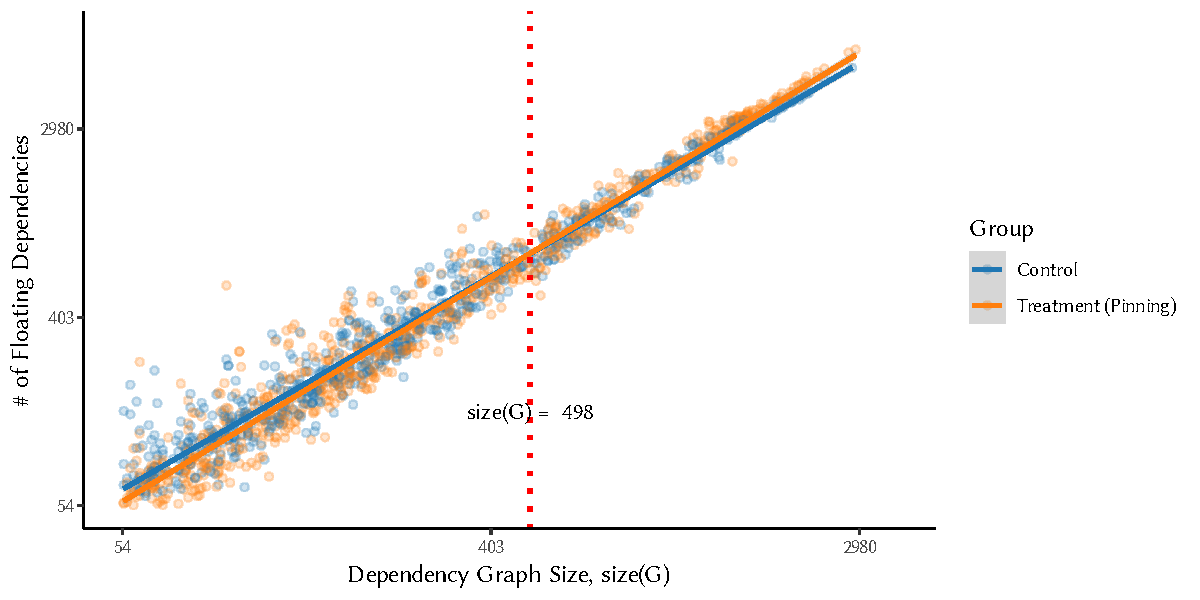
\includegraphics[width=0.9\linewidth]{figs-pinning/regression_n_floating.pdf}
    \caption{The effect of pinning direct dependencies on malicious package update attack surface (as measured by the number of floating dependencies in the entire dependency graph). Our model shows that pinning reduces attack surface for small dependency graphs, but the positive effect decreases as the dependency graphs grow larger and even flips to negative for dependency graphs with more than 498 dependencies.
    }
    \label{fig:n-floating}
\end{figure}

\section{RQ2:  How effective is coordinating pinning among selected upstream packages in reducing the risk of malicious package updates ecosystem-wide? }

As the results from RQ1  (Section~\ref{sec:results-rq2}) indicate, pinning direct dependencies is ineffective and possibly even harmful for preventing malicious package updates if a project has a large and complex dependency graph (we will return to this issue in Section~\ref{sec:pinning-discussion}). 
Then, a natural follow-up question arises: Are there better, alternative interventions that can effectively reduce the risk of malicious package updates in the npm ecosystem?
Inspired by previous research that reveals the structures of dependency networks~\cite{DBLP:journals/ese/DecanMG19, DBLP:conf/uss/ZimmermannSTP19}, we hypothesize that \emph{the risk of malicious package updates can be greatly reduced if a small set of ``core'' packages pin and promptly update all their dependencies after proper auditing} (ensuring there is no outdated dependency but also no malicious update).
That is, instead of all developers redundantly performing security actions, a few package maintainers (or a dedicated security team for the ecosystem) might effectively take on the cost of (some) security work by pinning and actively managing dependencies, so that all developers benefit. This would enable a vision where pooling some community resources would be much more efficient and effective to achieve security outcomes than trying to convince every single maintainer to change their practices (e.g., in a way similar to how the Linux Foundation starts the Core Infrastructure
Initiative in response to HeartBleed~\cite{DBLP:conf/msr/Walden20} or how Google provides the Assured Open Source Software service~\cite{assured-open-source}).
This leads to our RQ2 of exploring how coordinated pinning in select upstream packages may reduce the overall risk of malicious package updates at an ecosystem level.

\subsection{Method}
\label{sec:method-rq3}

\paragraph{Overview}
In a nutshell, we quantify the effect a few maintainers can have on %security outcomes 
the risk of (simulated) malicious package updates on the entire npm ecosystem.
We assume that we have the ability and budget to convince $n$ package maintainers of our choice to change their dependency management practices as follows: They pin each of their dependencies, review all dependency updates to catch malicious updates, and rapidly update all non-malicious updates.
This way, we would expect that some malicious updates are effectively detected by these $n$ maintainers, preventing them from affecting other developers in the ecosystem.
{Focusing on whether this approach is feasible at all, we make the following optimistic, simplifying assumptions: The $n$ maintainers review and update all dependencies immediately (without adding latency)
and they recognize all malicious package updates when they audit an update. %(100\% accuracy). 
We also assume that reporting and taking down a malicious package takes some time (\citet{DBLP:conf/dimva/OhmPS020} report a mean of 209 days), so even if some maintainers detect a malicious update and protect their users, others may still be exposed.
} 
Finally, we assume all other developers are floating all their dependencies, as they already mostly do. 

\paragraph{Dependency Network}
We simulate attacks on a snapshot of the package-level npm dependency network constructed from dependency relationships specified in the latest version of each package (cut-off in September 2023), using the same npm-follower dataset~\cite{DBLP:conf/sigsoft/PinckneyCG023} in Section~\ref{sec:data-collection}. 
The network has 1,566,434 packages (nodes) and 7,873,239 dependency edges.

\paragraph{Attack Selection Strategy}
In practice, attackers might target specific applications (e.g., specifically attacking cryptocurrency packages~\cite{crypto-attack}) or they may try to compromise whatever package they can to opportunistically cause damage (e.g., as common for untargeted ransomware attacks). Since we do not know what exact strategy attackers may pursue and since their strategy may change over time, we make the simplifying assumption that attackers will try to compromise high-impact targets by (randomly) selecting any of the top-$m$ packages (denoted as $A$) on npm as ranked by the downloads adjusted impact defined in Equation~\ref{eq:impact} (i.e., impact-based strategy).

\paragraph{Risk Metric}
Given the set $P$ of all packages in the network, we quantify the impact of compromising a package $a\in P$ as the download-weighted coverage of its reachable dependents within the entire npm network, where every package that depends directly or indirectly on package $a$ is considered reachable of the edge to $a$ in its dependency graph is floating:
\begin{equation}
\label{eq:impact}
    \textit{impact}(a)=\frac{\sum_{p \in \textit{reachable}(a)}\textit{downloads}(p)}{\sum_{p \in P}{\textit{downloads}(p)}}
\end{equation}
In other words, $\textit{impact}(a) \in [0, 1]$ measures the fraction of npm downloads that will be affected if package $a$ is compromised, as illustrated in Figure~\ref{fig:example-reachability}.

For the set of packages $A\subset P$ (i.e., the top-$m$ most impactful packages), in which an attacker may target any of $p \in A$ based on the attack selection strategy, we define \textit{risk(A)} as the arithmetic mean of the impact across all possible targets in $A$ an attacker can choose from (i.e., $\textstyle\textit{risk}(A)=\frac{1}{{|A|}}{\sum_{a \in A} \textit{impact}(a)}$).
% \begin{equation}
% \label{eq:risk}
%     \textit{risk}(A)=\frac{\sum_{a \in A} \textit{impact}(a)}{|A|}
% \end{equation}
Intuitively, $risk(A) \in [0, 1]$ is an estimation of the expected average percentage of npm downloads that would be affected by compromising any one of the packages in $A$.  

\begin{figure}[t]
    \centering
    \begin{subfigure}[b]{0.48\linewidth}
        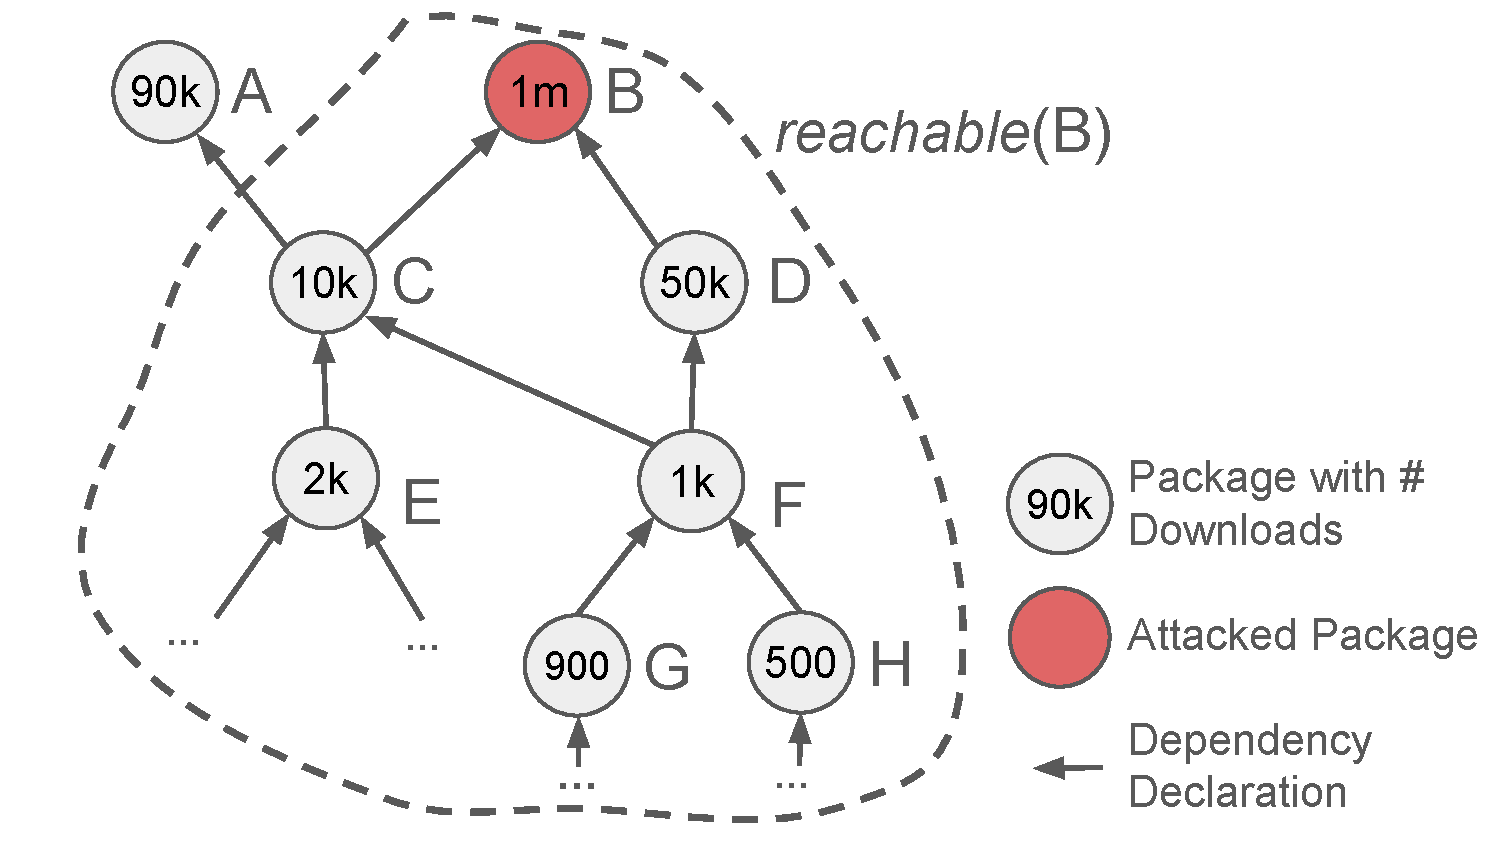
\includegraphics[width=\linewidth]{figs-pinning/example-reachability.pdf}
        \caption{\textbf{Attack Impact Computation:} Packages C to H all directly or indirectly depend on B and are hence reachable if B is attacked, but package A is not. The impact of compromising package B is the sum of downloads of all reachable packages (C--H) divided by the total number of downloads across all packages. In this case, $\textit{impact}(B) = (1m+10k+5k+2k+1k+900+500) / (90k+1m+10k+5k+2k+1k+900+500) \approx 0.92$.}
        \label{fig:example-reachability}
    \end{subfigure}
    \hfill
    \begin{subfigure}[b]{0.48\linewidth}
        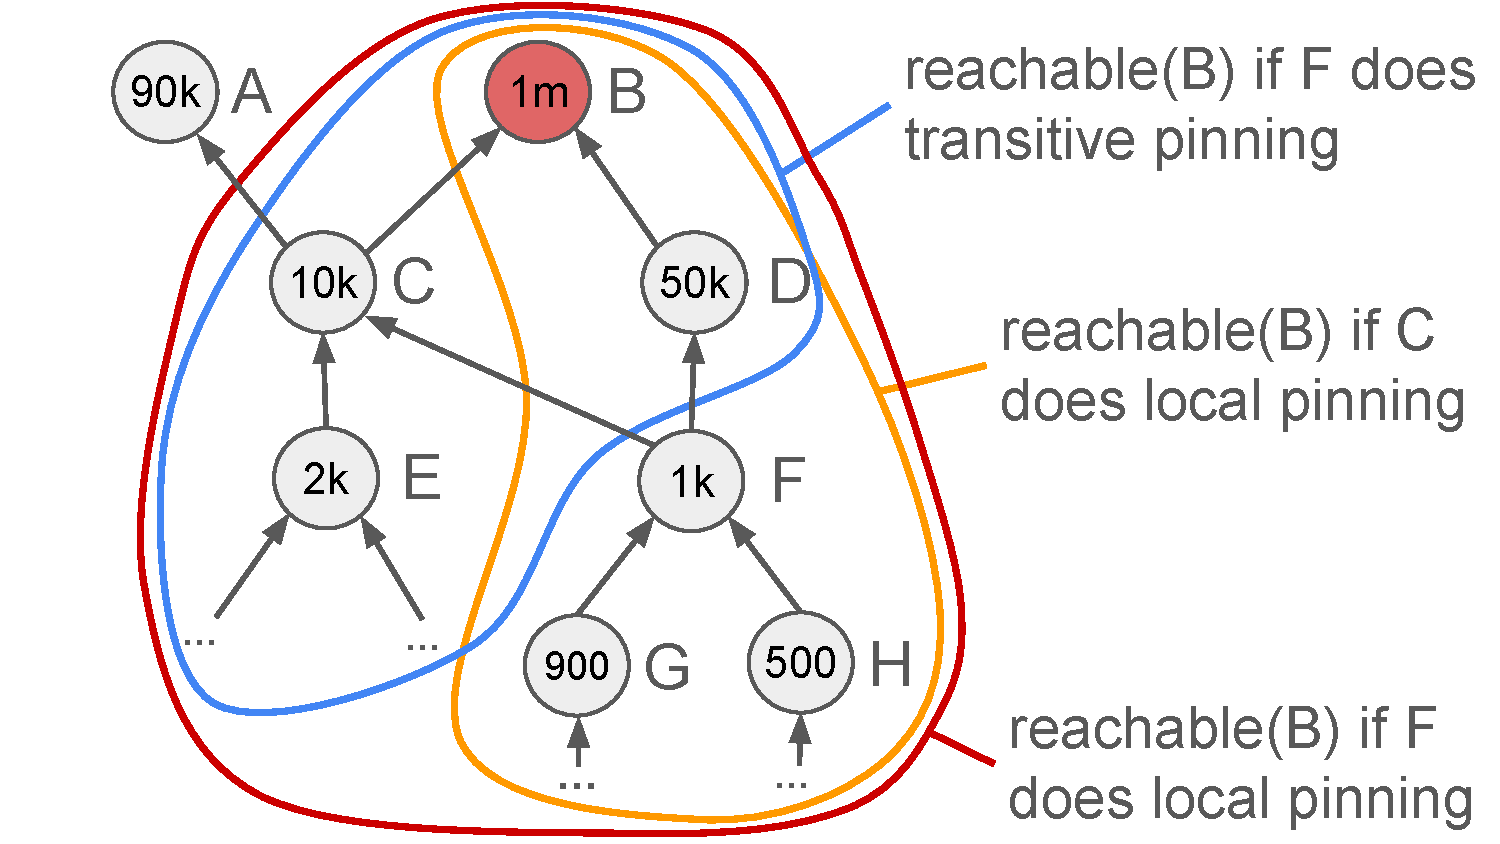
\includegraphics[width=\linewidth]{figs-pinning/example-transitive-pinning.pdf}
        \caption{\textbf{Local/Transitive Pinning:} Assume B is being attacked.
        If C pins its dependencies, the attack would not reach E, as C would not update to the malicious version. 
        However, local pinning of F would have no effect, since the attack still propagates through the floating edges originating from C and D. In contrast, transitive pinning of F would protect G and H (and F's other dependents) from the attack.}
        \label{fig:example-transitive-pinning}
    \end{subfigure}
    \vspace{-1mm}
    \caption{Examples to illustrate attack impact computation and how local/transitive pinning works.}
    \vspace{-1mm}
    \label{fig:example-rq3}
\end{figure}


\paragraph{Pinning Mechanism}
With npm's existing mechanisms, the maintainers of the $n$  defending packages can only pin their direct dependencies (\textit{local pinning}), but not their transitive ones. Maintainers can freeze their dependency graph with a \Code{package-lock.json} file, which, with npm's current design, only has an effect on their own package and not on anyone importing their package.

To give maintainers more power (at a higher maintenance cost), we imagine an alternative strategy of \textit{transitive pinning}, where maintainers can pin direct and indirect dependencies. This could be implemented with a 
% relatively local changes
change to npm that allows (a)~package maintainers to upload their \Code{package-lock.json} as part of the deployed package and (b)~npm to consider that file in each package during dependency resolution. We illustrate the difference in Figure~\ref{fig:example-transitive-pinning}.

\paragraph{Defense Selection Strategy}
Finally, we need to decide which $n$ packages to defend with local or transitive pinning.
Unfortunately, the problem of choosing an optimal package set of size $n$ that minimizes $risk(A)$ is equivalent to the Influence Minimization problem, which is NP-hard~\cite{DBLP:conf/icde/0002ZW0023}.
Hence, we focus on evaluating simple heuristics to choose the defended packages and leave the optimization as future work.
Specifically, we choose top-$n$ packages with (1) highest downloads, (2) highest out degrees (i.e., the packages with the most \textit{direct} dependencies), (3) highest betweenness centrality (i.e., the packages on most dependency \textit{paths}), (4) highest downloads $\times$ out degrees (i.e., popular packages with many direct dependencies), and (5) highest downloads $\times$ betweenness centrality (i.e., popular packages on many dependency paths).
Intuitively, we expect defense selection strategies based on out degree to work best for local pinning as they emphasize direct dependencies, and strategies based on betweenness to work best for transitive pinning as transitive pinning interrupts paths.

\paragraph{Simulation}
For each combination of pinning mechanism, defense selection strategy, and number of defended packages from 0 to $n$, we measure the impact of the defense on the risk metric. To compute the impact, we compute \textit{risk(A)} with a modified \textit{reachable} function (Equation~\ref{eq:impact}, different from the standard notion of graph reachability) by breaking propagation of the attack when the final edge is pinned (local pinning) or if the path contains a defended package (transitive pinning).

\paragraph{Limitations and Threats to Validity}
To make the simulation feasible, we make several simplifying assumptions described above.
Notably, we assume that  attacks happen uniformly randomly on a fixed number of attack targets, while real attack selection strategies may be more targeted, more opportunistic, and may adapt in response to defense strategies.
Therefore, we additionally explored two different attack selection strategies: (1) attacking any actively maintained projects randomly, and (2) attacking the most fragile or under-maintained packages (e.g., as the \Code{xz} attack, which focused on a dependency with a single overworked maintainer~\cite{xz-utils}) defined as the bottom-1000 packages in our package dataset, ranked by the number of core maintainers estimated in World of Code~\cite{DBLP:journals/ese/MaDBAVTKZM21}. For space and since our results are generally robust under the different attack selection strategies, we only report results under the impact-based attack selection strategy (the remaining are in the replication package, Section~\ref{sec:data-availability}).
What's more, the dependency network is only an approximation of reverse dependency relationships. 
However, similar kinds of dependency networks are frequently used in prior research~\cite{DBLP:journals/ese/DecanMG19, DBLP:conf/uss/ZimmermannSTP19} because it is generally impossible to compute precise reverse dependencies as would be resolved by npm due to its deduplication optimizations (Section~\ref{sec:background}).
For defense selection strategies, we have to rely on simple heuristics, leaving potentially better strategies (e.g., more computationally expensive optimization attempts) to future work.
Finally, due to a lack of access to real-world application data, our simulation does not accurately quantify the impact of malicious package updates on applications, whether open-source repositories or closed-source projects outside of npm.
We mitigate this by considering downloads in attack impact estimation (Equation~\ref{eq:impact}), but npm download data can be also noisy and inconsistent.
%As in RQ 1 and~2, our results are specific to the structure and practices of the npm ecosystem.
Due to these simplifying assumptions, readers should take our results as a first exploration of broad defense strategies and their ecosystem-wide effects, rather than specific implementation recommendations.

\subsection{Results}
\label{sec:results-rq3}

\begin{figure}[t]
    \centering
    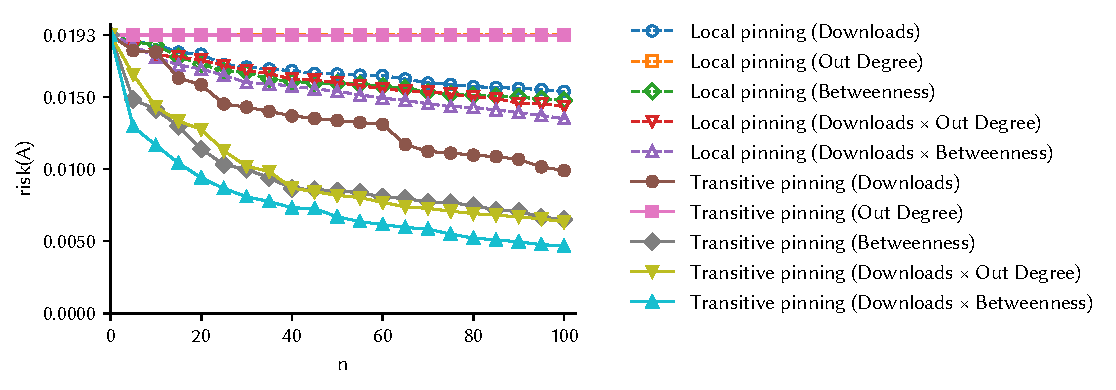
\includegraphics[width=0.98\linewidth]{figs-pinning/intervention_top_1000.pdf}
    \vspace{-3mm}
    \caption{The reduction of malicious package update risk ($risk(A)$) by securing top $n$ packages with five different defense selection strategies using local pinning and transitive pinning, respectively.}
    \label{fig:intervention}
\end{figure}

In this section, we report results for $n = 100$ and $m=1,000$ (i.e., defending up to 100 packages to minimize the risk of attack among the top 1000 most impactful packages; the results are robust under other $n$, $m$ variations which are available in the replication package, Section~\ref{sec:data-availability}).
As visible in Figure~\ref{fig:intervention}, one would expect 1.93\% of npm downloads to be affected on average upon an attack without any intervention, which is enormous considering that npm has  $\sim$12 billion downloads per day in 2024~\cite{sonatype-report}.
Most defense strategies can reduce ecosystem-wide risk (from  doing nothing at $n=0$) with targeted defenses at 10 to 100 packages, but their effectiveness varies widely. The best local pinning strategy can reduce ecosystem-wide risk against the 1000 most popular packages by 12.21\% with defending only 20 packages and 30.09\% when defending 100 packages. 
The best transitive pinning strategy can reduce ecosystem-wide risk against the 1000 most popular packages by 51.34\% when defending only 20 packages and 75.81\% when defending 100 packages.
For both pinning mechanisms, selecting packages with betweenness weighted by downloads is most effective,
but transitive pinning is usually two to three times more effective than local pinning. 

\section{Discussion}
\label{sec:pinning-discussion}

\subsection{Why can pinning direct dependencies lead to a larger total number of floating dependencies (i.e., a larger attack surface for malicious package updates)?}

\begin{figure}[t]
    \centering
    \begin{subfigure}[b]{0.46\linewidth}
        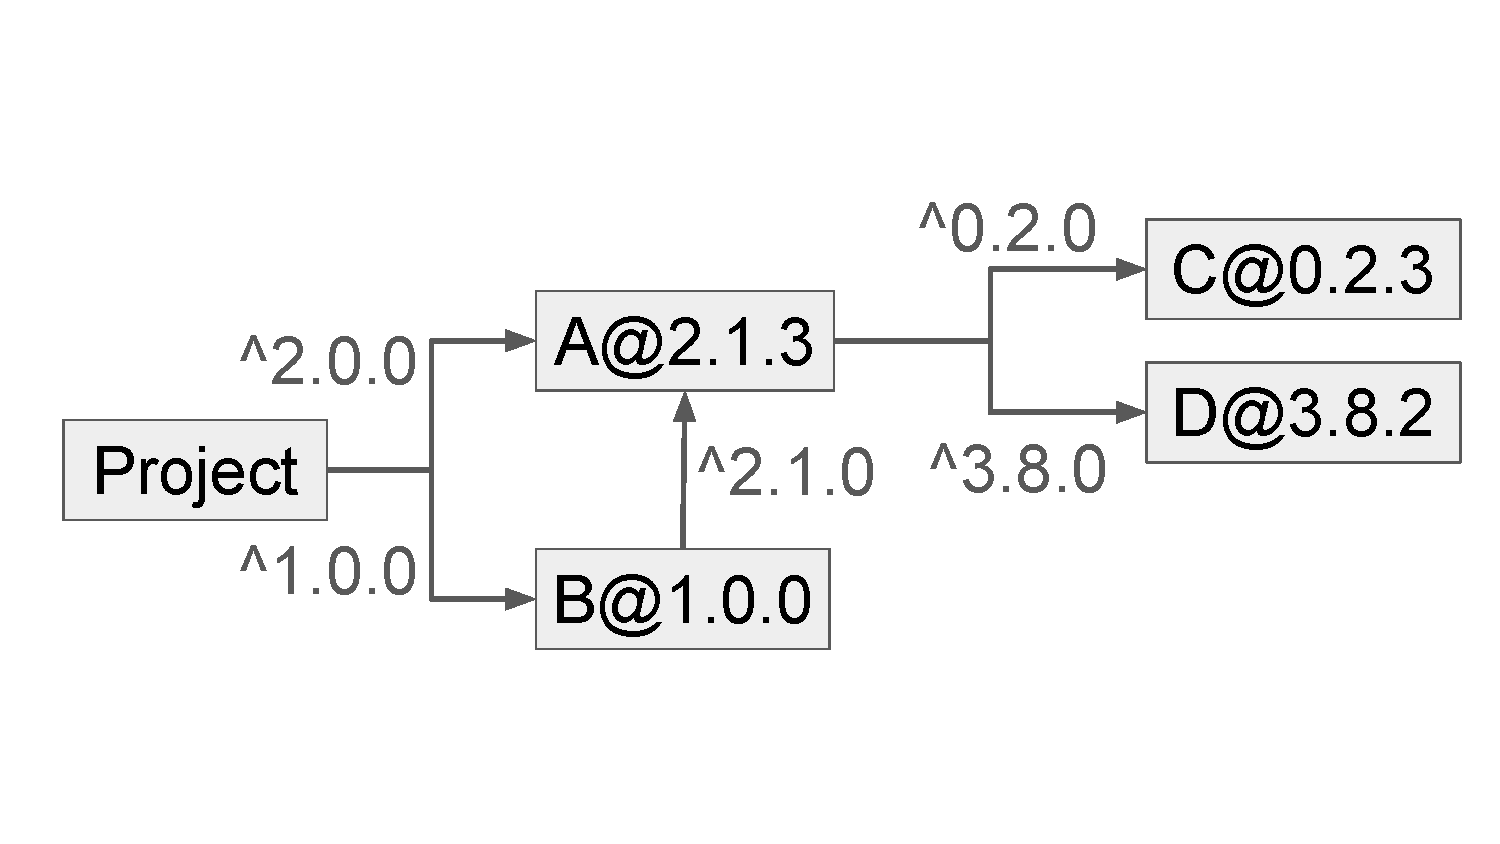
\includegraphics[width=\linewidth]{figs-pinning/example-wo-pinning.pdf}
        \caption{Not pinning (\textbf{5} floating edges)}
        \label{fig:floating-example}
    \end{subfigure}
    \begin{subfigure}[b]{0.46\linewidth}
        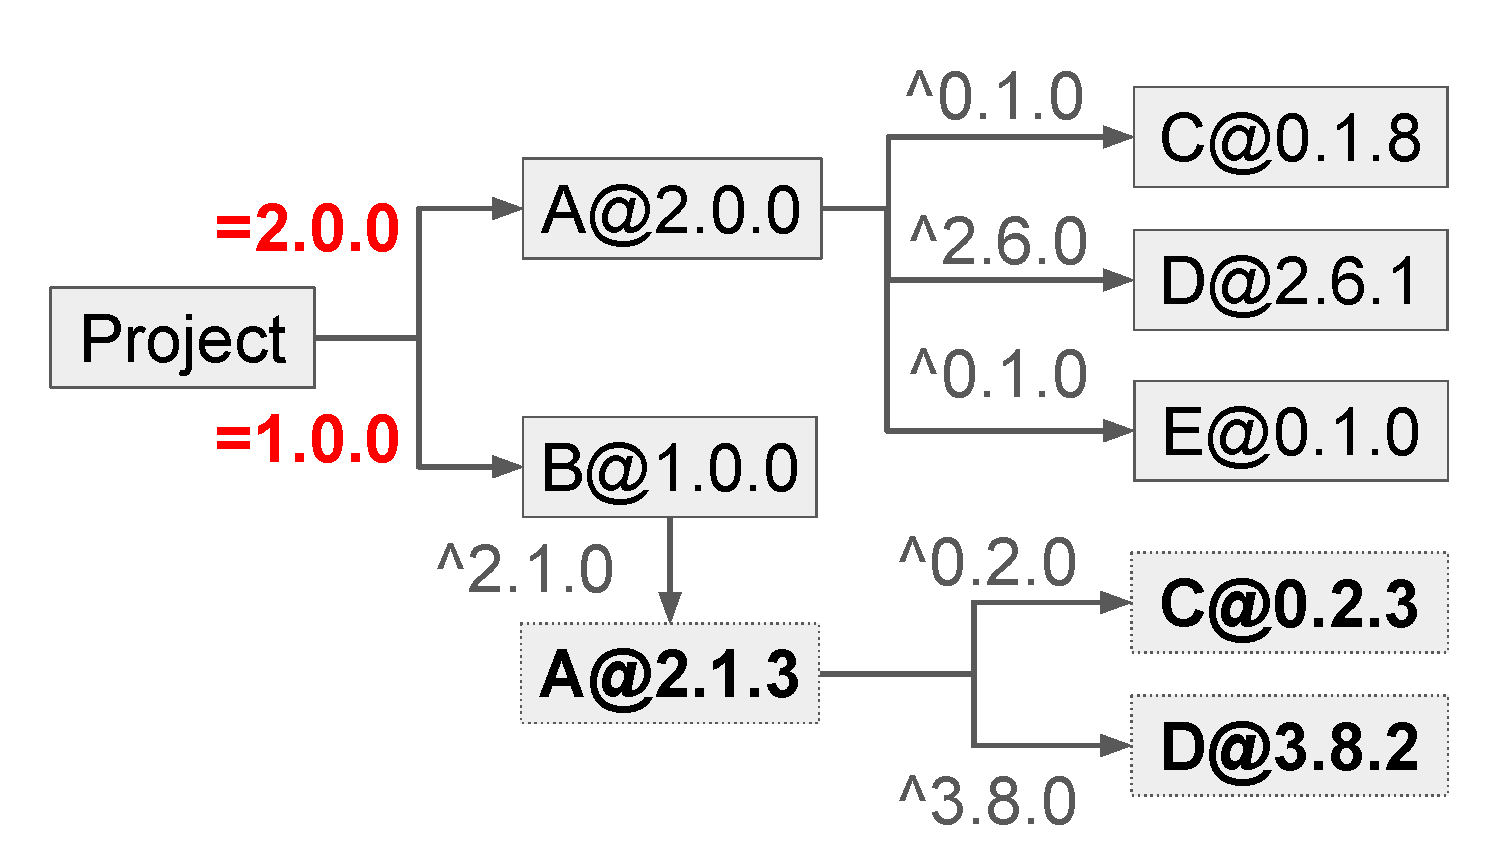
\includegraphics[width=\linewidth]{figs-pinning/example-with-pinning.pdf}
        \caption{Pinning (\textbf{6} floating edges)}
        \label{fig:pinning-example}
    \end{subfigure}
    \vspace{-1mm}
    \caption{A minimal example illustrating how pinning direct dependencies can cause dependency conflicts and lead to a bloated dependency graph with more transitive floating dependencies. Note that this is only an artificial example for simplicity; real-world cases happen mostly in much larger dependency graphs.
    }
    \vspace{-1mm}
    \label{fig:rq2-example}
\end{figure}

\label{dedup}
This surprising effect is explained by a detail of how the npm dependency resolver handles dependency conflicts~\cite{how-npm3-works} (cf. Section~\ref{sec:background}):
If two or more nodes in the dependency graph declare a dependency  on the same package, npm will first check (with heuristics) whether there is a version of that package that meets all declared version constraints (as in our example in Figure~\ref{fig:floating-example}). If there are conflicting version constraints in dependency declarations, npm will install multiple versions of the package to satisfy all version constraints (as in our example in Figure~\ref{fig:pinning-example}). This deduplication (or debloating) process is designed to download fewer, often redundant, copies of packages in the installation process. In fact, there are many possible deduplication heuristics and researchers have explored how to improve this in various ways (e.g., using an SMT solver~\cite{DBLP:conf/icse/PinckneyCGBCG23}).

The deduplication process interacts with pinning: If more dependencies are pinned, the dependency graph resolution has fewer opportunities to deduplicate a specific package and will be more likely to create larger dependency graphs with multiple versions of the same package. Those different versions may also then include additional dependencies---as visible in our example in Figure~\ref{fig:rq2-example}. Both effects increase the attack surface, in that attackers have possibly more version ranges they can attack for the same packages and there could be even additional packages they can attack.
This leads to our conclusion that \textit{the practice of (local) pinning is futile and even counter-productive for the purpose of reducing floating dependencies (aka attack surface) in one's dependency graph}.

Note that the deduplication heuristics introduced here and the ability to install multiple versions of the same package are unique to npm~\cite{DBLP:journals/tosem/BogartKHT21}.
In most other dependency managers, the resolver must find a single version for each package and pinning can make this much harder (as captured also in our \Code{n\_bloated} metric for pinning).
In those ecosystems, pinning would arguably still have only marginal effects on attack surface reduction, but not negative ones.
However, the costs for resolving dependency conflicts would be much more substantial~\cite{DBLP:conf/sigsoft/WangWLWWYYZC18, DBLP:conf/icse/WangW0WLWYCX020}. 

\subsection{Implication for Practitioners}

\textbf{Dependency pinning is (as expected) an expensive intervention.}
Regarding the drawbacks of pinning, our RQ1 results align with the argued trade-offs in Table~\ref{tab:trade-offs}:
Pinning direct dependencies substantially increases the effort for developers to manually update (and possibly review) dependencies if they want to stay up to date, or face many outdated dependencies if they do not. 
Also, projects that pin their dependencies are, as expected, much more likely to be exposed to known vulnerabilities in their dependency graph if they do not constantly update to available patches. While bots and notification tools like \textit{Dependabot} can help with some of that work and even automatically run tests and merge updates (as covered in prior work~\cite[e.g.,][]{mirhosseini2017can,DBLP:conf/msr/AlfadelCSM21}), they also have their limitations, creating additional complexity (e.g., notification fatigue~\cite{DBLP:conf/sigsoft/HeHGZ21}).

\textbf{Pinning direct dependencies is futile and (surprisingly) can be even counter-productive as a security intervention if floating is the mainstream practice in the ecosystem.}
Our RQ1 results regarding the expected security benefits of pinning are surprising and counter-intuitive to practitioners (based on our experience when sharing the results).
The first reason is that in many projects, direct dependencies are far outnumbered by transitive dependencies for which version declarations are controlled by upstream packages (Table~\ref{tab:dataset}). 
Thus, the action of a single project has a relatively small impact on the total number of floating dependencies in its dependency graph, explaining the small effective size and the diminishing return of pinning as the dependency graph grow larger (as confirmed by the interaction term $\text{\emph{pinning}} \times \ln(size(G))$ in our panel regression model and illustrated visually in Figure~\ref{fig:n-floating}).
Importantly, the security benefit of pinning does not only diminish, but it \textit{reverses} and pinning becomes actually counterproductive in large dependency graphs ($\ge$498 nodes according to our model, also visible as a crossover point in Figure~\ref{fig:n-floating}), to the point that \textit{pinning direct dependencies leads to more floating dependencies in the entire dependency graph.}  
In other words, an attacker may be able to attack the same dependencies in more version ranges or may even be able to attack additional dependencies that are only (indirectly) included in some versions of some dependency.
More generally speaking, the perceived security trade-off between pinning (to reduce the risk of malicious updates) and floating (to get fewer security vulnerabilities) does not hold in practice if the upstream packages are mainly floating (e.g., in npm and PyPI). 

Following the discussion above, \textbf{in an ecosystem where floating is the mainstream practice, pinned dependencies do not necessarily signal that a project is more secure from malicious package updates, especially for projects with large dependency graphs.}
In such contexts, pinning can create substantial maintenance costs, for limited security benefits, if any. 
Therefore, we argue that pinning should not be considered when scoring the security practices of packages.

\textbf{Instead of pinning, application developers should freeze their entire dependency graph with a shared lock file.}
In the npm ecosystem, it means using and \emph{commiting} the \Code{package-lock.json} file (Section~\ref{sec:background}) to the version control repository (44.21\% of GitHub repositories in our dataset did this).
This practice enables the effective pinning of all direct and transitive dependencies and more importantly, prevents updates from being installed automatically in a new machine or in the CI/CD environment.
However, \emph{lock files are intended only for applications (not packages)}, and they are not designed to allow easy selective updates or audits of dependency updates---hence every developer would need to individually judge when to update which (possibly indirect) dependencies rather than delegating some of that judgment to package maintainers and ecosystem moderators.

\textbf{To secure an ecosystem from supply chain attacks, package developers may consider community-wide coordination from a collective pool of resources.}
For example, our RQ2 results indicate that collective pinning actions could indeed be fairly effective at reducing the risk of malicious package updates and \textit{localize} the cost to a few (20--100) carefully selected packages.
We believe it is much more achievable to convince (and raise labor or funds for) changing practices in 100 packages for the good of the entire ecosystem, than trying to convince almost every maintainer in npm individually to change their practices.
However, our results also show clearly that npm's current local pinning is far less effective than transitive pinning could be. 
While transitive pinning is far more expensive for the maintainer defending a package (i.e., they need to audit updates of transitive dependencies too, not just of direct ones), it also provides a bigger lever for security. 
Transitive pinning is also easier to explain to developers, whereas local pinning can provide a false sense of security with counter-intuitive consequences (as shown in our RQ1).
Therefore, \textbf{we suggest changes to npm infrastructure and tooling to enable transitive pinning (e.g., publishing a \Code{package-lock.json} file for downstream consumption).}

However, we must note that these kinds of interventions would probably still experience pushback and be costly to implement from such an established ecosystem (as of pushing any organizational change~\cite{schein2010organizational}).
To make the process easier, \textbf{we encourage foundations, security companies, or companies using open source to dedicate resources (labor, funds) to such efforts}.
Even if only a small number of maintainers opt to purse this (i.e., transitive pinning and extensively review their updates), it can have a large impact on the ecosystem.

Finally, it is worth noting that the whole debate around version constraints relies on one critical assumption: \emph{malicious package updates will go undetected in the ecosystem for a significant amount of time}, which is probably still the case as of now (as evidenced by the \Code{xz} attack~\cite{xz-utils}).
If malicious package updates are taken down faster or even stopped before being published in the package registry, their impact  will be much smaller.
Thus, \textbf{efforts are needed to make malicious package updates as short-lived as possible.}
We envision that if a small number of core ecosystem packages can pin and \emph{promptly review their updates}, they can also help in such early detection, for example, by leveraging the ongoing research about detecting malicious packages~\cite[e.g.,][]{DBLP:conf/icse/SejfiaS22, DBLP:journals/corr/abs-2403-12196}.

\subsection{Implication for Researchers}

Our study leaves a few open research questions.
First, our study only focuses on the npm ecosystem, and other ecosystems adopt different baseline dependency versioning practices~\cite{DBLP:journals/tosem/BogartKHT21, DBLP:conf/msr/0001PSTB19}.
Future research is necessary to explore the impact of pinning/floating under those variations.
Second, while prior research provides evidence that floating jeopardizes build stability~\cite[e.g.,][]{DBLP:conf/issta/MukherjeeAR21}, the \Code{n\_auto\_update} model in RQ1 only explains a small amount of variance in the data ($R^2$<0.1), so we expect future work to better establish the causal relationship between pinning and application stability.
Third, our RQ2 only takes a first step to explore possible ecosystem-level strategies, and we encourage more research in this direction. 
We suggest exploring better strategies than download-weighted betweenness and exploring how to consider users of packages outside npm.  
Researchers may also explore alternative simulation approaches going beyond our simplifying assumptions, and, for example, consider the specific existing choices of pinning and floating in the dependency graph when suggesting which packages to defend. 
Future research could also explore whether these strategies hold when baseline pinning and floating practices are different in other ecosystems~\cite{DBLP:journals/tosem/BogartKHT21, DBLP:conf/msr/0001PSTB19}.
Another remaining question is whether a maintainer's decision to pin their package's dependencies produces unintended non-local costs for package users. 
For example, it is possible that the pinning in some parts of the dependency graph can affect users negatively in terms of causing them dependency conflicts (cf. \Code{n\_bloated} in Section~\ref{sec:results-rq2}). 
Researchers may explore whether different defense selection strategies (e.g., explicitly coordinating dependency updates across packages) or explicitly advocating for floating outside of a few defended packages can reduce unintended dependency conflicts.
Again, we expect all these concerns to manifest differently in different ecosystems and we envision a broad range of future research to establish the security impact of versioning practices in a wide variety of contexts.

\section{Conclusion}

In this paper, we have presented a counterfactual analysis and simulation study on the impact of version constraints in the npm ecosystem.
We have explored the security and maintenance impact of local pinning direct dependencies and the effectiveness of pinning on ``important'' packages against possible malicious package updates.
Our study provides counter-evidence for the use of local pinning as a security best practice, but supports the effectiveness of coordinated pinning in critical open-source packages.
Our study leads to a series of implications for the design of dependency management tools and ecosystem-level coordination to enhance software supply chain security.

\subsubsection*{\textbf{Data Availability}}
\label{sec:data-availability}

We provide a replication package at \url{https://doi.org/10.5281/zenodo.14693233}.

\subsubsection*{\textbf{Acknowledgement}}

He's and Kästner's work was supported in part by the National Science Foundation (award 2206859).
Bogdan's work was supported in part by the National Science Foundation (award 2317168) and research awards from Google and the Digital Infrastructure Fund.
We would like to thank James Herbsleb, Narayan Ramasubbu, Rohan Padhye, and the participants of S3C2 quarterly meetings for their valuable feedback to the earlier versions of this work. 



\chapter{Empirical Study II: The Impact of Fake GitHub Stars on Repository Promotion}
\label{chp:fake-stars}

\section{Introduction}
\label{sec:introduction}

\begin{quote}
\emph{
The more any quantitative social indicator is used for social decision-making, the more subject it will be to corruption pressures and the more apt it will be to distort and corrupt the social processes it is intended to monitor.
}
- Donald T.\ Campbell~\cite{campbell1979assessing}
\end{quote}

\begin{figure}
    \centering
    \begin{subfigure}{0.37\linewidth}
        \centering
        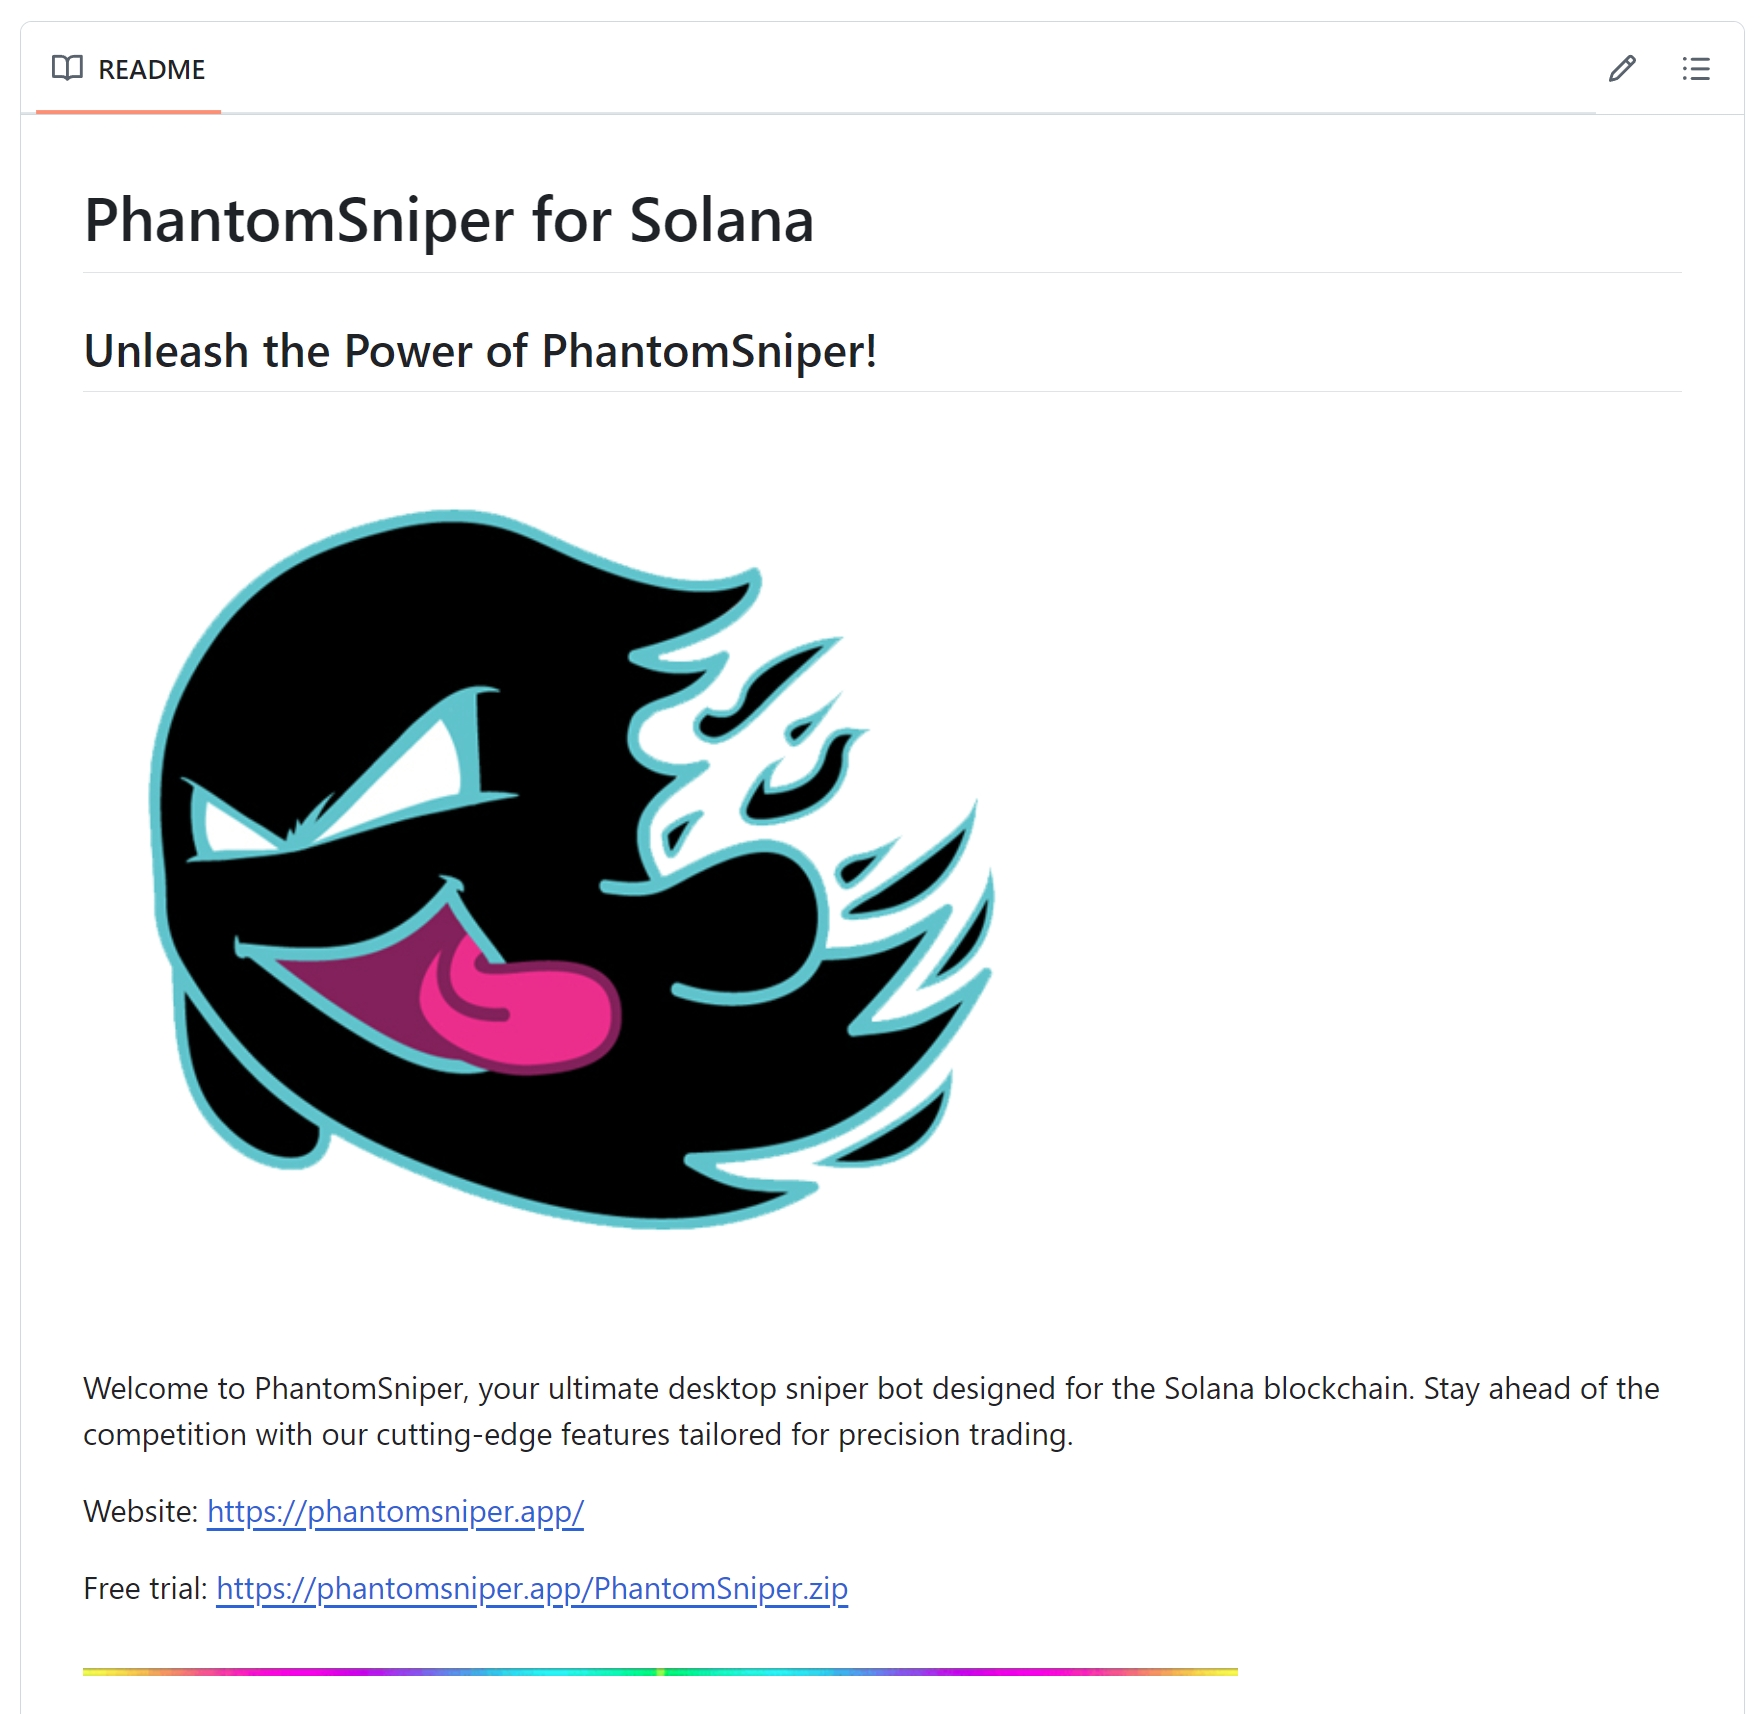
\includegraphics[width=\textwidth, clip=true, trim=85 260 350 180]{figs-fake-stars/malware-example4.png}
    \end{subfigure}
    \begin{subfigure}{0.6\linewidth}
        \centering
        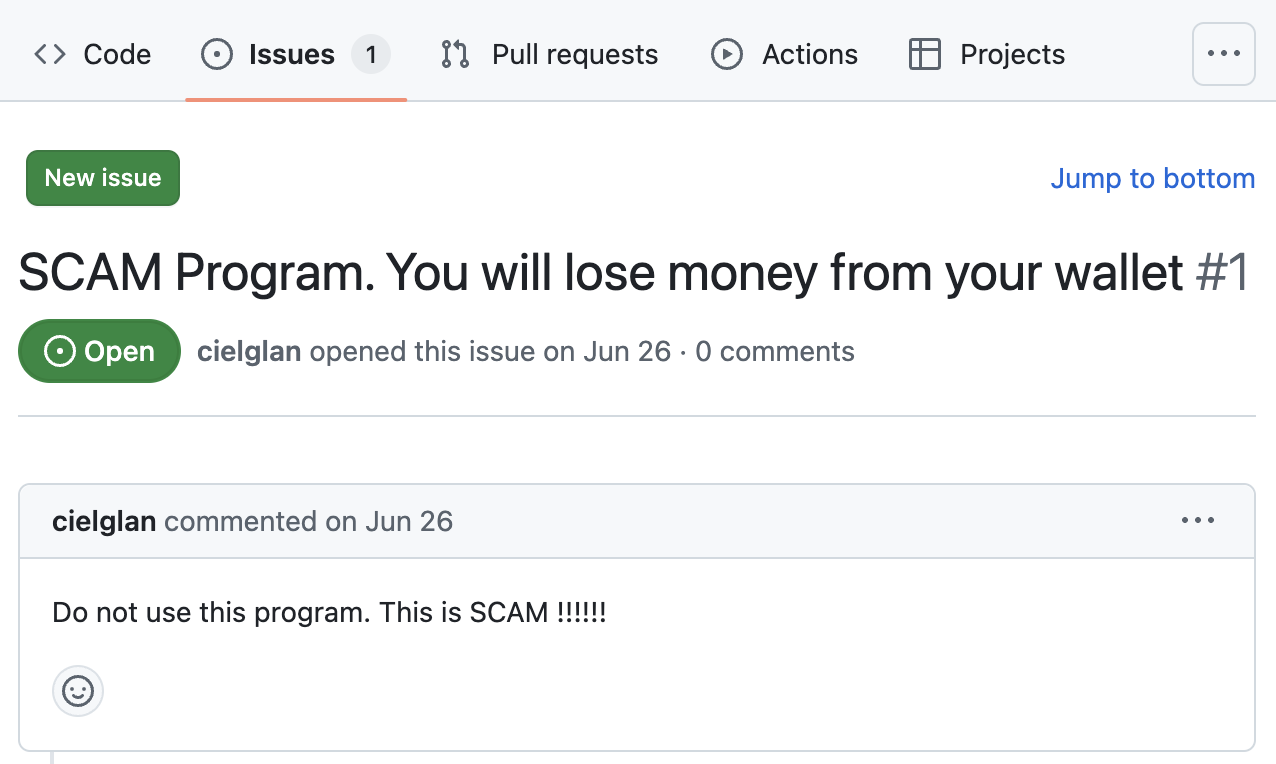
\includegraphics[width=\textwidth]{figs-fake-stars/malware-example6.png}
    \end{subfigure}
\begin{minted}[
frame=lines,
framesep=2mm,
baselinestretch=1,
fontsize=\scriptsize,
]{javascript}
// main.js, hidden at line 12 starting at column 892
const {spawn}=require('child_process');const cmd1='node';
const argv1=['node_modules/@solana-web3-1.43.js'];
spawn(cmd1,argv1,{detached:true,windowsHide:true});
// node_modules/@solana-web3-1.43.js
...;const axios=require('axios'),AdmZip=require('adm-zip'),
fs=require('fs'),{exec}=require('child_process');...;
async function downloadFile(){const _0x3cefa0={'mgLtL':
function(_0x340848,_0x3c32b9){return ...;}}...};
\end{minted}
    \caption{An example malware repository detected by our tool \SystemName, reported to GitHub, and since deleted. It had 111 stars, of which we suspect at least 109 to be fake. The README file (top left) suggests a blockchain application, but if executed, its code (bottom) steals cryptocurrencies using a hidden \Code{spawn()} call to a heavily obfuscated remote file execution script (with the name of a seemingly legitimate JavaScript package). An issue thread (top right), presumably created by a victim, warns of malware hidden inside.}
    \label{fig:malware-example}
\end{figure}

Many studies provided evidence that the number of GitHub stars is widely used when stakeholders evaluate, select, and adopt open-source projects into their software supply chain~\cite{DBLP:journals/jss/BorgesV18, DBLP:journals/pacmhci/QiuLPSV19, DBLP:conf/sigsoft/VargasATBG20, DBLP:journals/ese/MunaiahKCN17,  DBLP:conf/sp/WermkeWKFAF22, koch2024fault}.
However, it is merely a popularity signal (i.e., the attention received from GitHub users), with only moderate correlation to actual usage or importance as shown in prior studies~\cite{koch2024fault, schueller2024modeling, DBLP:journals/corr/abs-2405-07508}. 

More concerning, \emph{GitHub stars can be artificially inflated}~\cite{wired-news}, just as all other popularity signals in social media~\cite{DBLP:journals/compsec/CatalanPVT23}.
For example, a Google search for ``buy GitHub stars'' will reveal a dozen providers (see Appendix, Section~\ref{sec:conclusion}).
From prior reports, we know that GitHub repositories may buy GitHub stars for growth hacking~\cite{oceanbase}, spamming~\cite{dagster}, r\'{e}sum\'{e} fraud~\cite{DBLP:conf/acsac/DuYZDWH0020}, or even for spreading malware~\cite{stargazer-goblin}.
Whatever their purpose, these bought GitHub stars (hereafter ``fake stars'' to match online discussions) corrupt the GitHub star count as a decision-making signal and pose a security threat to all GitHub users (see Figure~\ref{fig:malware-example} for an example).

However, most prior reports of fake GitHub stars come from the gray literature (i.e., non-peer-reviewed blog posts, news reports, and online discussions), and they do not go beyond studying a few specific cases~\cite{dagster, DBLP:conf/acsac/DuYZDWH0020, oceanbase, stargazer-goblin}.
With the rising prevalence of software supply chain attacks~\cite{sonatype-report}, we believe it is important to conduct \emph{a systematic, global, and longitudinal measurement of this emerging threat, especially from the lens of software supply chain security}.
This would contribute to our understanding of fake GitHub stars and the fraudulent/malicious activities around them, furthering the design of countermeasures and informing best practices on the usage of an important software supply chain metric.

Several challenges persist in the global measurement of fake GitHub stars.
First, GitHub stars can be faked in various ways (e.g., bots~\cite{stargazer-goblin}, crowdsourced humans~\cite{oceanbase}, exchange platforms where users exchange stars for a reward~\cite{DBLP:conf/acsac/DuYZDWH0020}), and malicious actors continuously evolve their behaviors to evade platform detection~\cite{DBLP:journals/tissec/IkramOFCFJKS17, DBLP:conf/www/CresciPPST17}.
Their actions blur the boundary between fake and authentic stars, posing a challenge to the identification and measurement of fake ones.
Second, the sheer amount of GitHub data ($\sim$20TB of metadata in the past five years~\cite{gharchive}) and the rate limit of GitHub APIs~\cite{github-rest-api} present challenges to a global analysis.
Finally, GitHub does not preserve deleted repositories and users, posing difficulties in the measurement of fraudulent or malicious activities, as some of them may have already been taken down by the platform.

To overcome these challenges, we take advantage of prior work on mining software repositories~\cite{gharchive} and social media fraud detection~\cite{DBLP:conf/www/BeutelXGPF13, DBLP:conf/www/CresciPPST17} to implement \SystemName, a scalable tool that detects (suspected) \emph{fake stars} over the entire \textsf{GHArchive}~\cite{gharchive} dataset, a Google BigQuery replica of all GitHub events (totaling 63.9 million users, 331 million repositories, 326 million stars, and 6.7 billion other events as of January 2025).
\SystemName (details in Section~\ref{sec:tool-design}) identifies two signatures of anomalous starring behaviors, \emph{the low activity signature} and \emph{the lockstep signature}, and includes a post-processing step to reduce noise and increase overall accuracy.\footnote{
Note that technically speaking, \SystemName only detects \emph{suspected} fake stars and \emph{suspected} fake star campaigns, among which there may still be false positives (see Section~\ref{sec:limitations} for a discussion).
However, to make this paper more readable, we will simply refer to them as \emph{fake stars} and \emph{fake star campaigns} in the remainder of this paper.
}

We apply \SystemName to all GitHub event data from July 2019 to  December 2024, identifying \emph{6.0 million fake stars and 18,617 repositories with fake star campaigns}.
Our evaluation shows that: (a)~\SystemName can detect 81\% of repositories and 76\% of accounts in a confirmed malware campaign involving fake stars~\cite{stargazer-goblin}; (b)~the detected repositories and accounts have anomalously high deletion ratio, up to 90\%, 16x higher compared to random GitHub repositories and accounts.

Using the dataset, we further conduct a measurement study that answers the following research questions:
\begin{itemize}[leftmargin=15pt]%,itemsep=2pt]
    \item \RQOne
    \item \RQTwo
    \item \RQThree
    \item \RQFour
\end{itemize}

Our findings paint an alarming picture: Fake stars have surged in 2024, either to promote spam or phishing malware repositories, or fuel popularity contests in hyped domains (e.g., blockchain and AI). 
In the latter case, we show that fake stars, while increasing the displayed star counts in the short term, fail to bring true attention in the long term.
From a security perspective, our results call for future research into malicious activities happening on GitHub (e.g., fake stars, fake accounts, spam, phishing).
From a practitioner's perspective, our results further demonstrate the limitation of star counts as a popularity signal, provide counter-evidence to the effectiveness of fake stars for growth hacking, and call for the design of better popularity signals for GitHub repositories.

In summary, this paper makes the following contributions:
\begin{itemize}[leftmargin=15pt]
    \item We design and implement \SystemName, a scalable tool to scan for anomalous starring behavior across all of GitHub.
    This leads to a novel large-scale dataset regarding fake GitHub stars.
    \item Our measurement study discovers novel findings regarding the prevalence, characteristics, and effectiveness of fake stars, leading to practical insights for platform moderators, open-source practitioners, and supply chain security researchers.
\end{itemize}

\section{Background and Related Work}

GitHub is the de facto platform where developers collaborate in open-source projects (organized as \emph{repositories}).
It is designed to be transparent, and repositories can build their reputation through technical and social signals (e.g., stars, forks, badges)~\cite{DBLP:conf/icse/TrockmanZKV18, DBLP:conf/icse/TsayDH14}.
As the design of these social signals resembles those in online social networks, we first introduce spam/fraud research there (Section~\ref{sec:fake-activity}).
Then, we introduce software supply chain attacks (Section~\ref{sec:supply-chain-security}) and summarize prior findings on (fake) GitHub stars (Section~\ref{sec:github-stars}).

\subsection{Fraudulent Activities in Social Networks}
\label{sec:fake-activity}

In a nutshell, most of the fraudulent activities in online social networks are about controlling a group of fake accounts to spread spam or generate fake signals.
There is a rich literature on countering fraudulent activities in online social networks (see, e.g., recent literature reviews~\cite{DBLP:journals/eswa/Latah20, DBLP:journals/eswa/RaoVB21, DBLP:journals/snam/AljabriZSASA23}).
For example, researchers have studied how fake accounts can be used to spread advertisements~\cite{DBLP:conf/imc/ThomasGSP11}, malware~\cite{DBLP:conf/ccs/GrierTPZ10}, misinformation~\cite{shao2018spread}, and political opinions~\cite{faris2017partisanship, pierri2020investigating}.
They can also be used to artificially boost the popularity of posts or users (using, e.g., fake Likes in Facebook~\cite{DBLP:conf/www/BeutelXGPF13, DBLP:journals/tissec/IkramOFCFJKS17} and Instagram~\cite{DBLP:conf/websci/SenAMSKD18}, and fake followers and retweets in Twitter~\cite{DBLP:conf/imc/StringhiniWEKVZZ13, DBLP:conf/ccs/SongLK15}).
For the latter scenario, a recurring observation from prior research is that some providers generate fake popularity signals using automated bots (aka. sybils), but some others use realistic accounts and even crowdsourced real humans (aka. crowdturfing)~\cite{DBLP:conf/imc/StringhiniWEKVZZ13, DBLP:conf/www/WangWZZMZZ12,DBLP:journals/tkdd/YangWWGZD14, DBLP:conf/ccs/SongLK15, DBLP:journals/tissec/IkramOFCFJKS17}. 

With a ground truth dataset and reasonable feature engineering, it is often possible to build high accuracy supervised machine learning models to detect such activities~\citep[e.g.,][]{DBLP:conf/imc/StringhiniWEKVZZ13, DBLP:conf/ccs/SongLK15, DBLP:conf/ccs/XiaoFH15}, but these models can be evaded by malicious actors if they change their behaviors over time~\cite{DBLP:conf/uss/WangWZZ14, DBLP:conf/www/CresciPPST17}.
Another line of research uses unsupervised techniques to detect anomalous users and activity clusters that deviate significantly from normal ones~\cite{DBLP:conf/www/BeutelXGPF13, DBLP:conf/ccs/CaoYYP14, DBLP:conf/uss/ViswanathBCGGKM14, DBLP:conf/kdd/HooiSBSSF16}.
However, \citet{DBLP:journals/tissec/IkramOFCFJKS17} show that the Facebook Like farms are still able to maneuver through these techniques by mimicking realistic user activities and violating the techniques' built-in assumptions (e.g., assuming that fake Likes happen in bursts~\cite{DBLP:conf/www/BeutelXGPF13}).
In general, the battle against fraudulent activities in social media is a never-ending arms race~\cite{DBLP:conf/www/CresciPPST17, yang2019arming}.
Our study contributes to this literature by providing a systematic report of an emerging fraudulent activity (i.e., fake stars) in a novel setting (i.e., GitHub, the de facto social coding platform for open-source projects).

\subsection{Software Supply Chain Attacks}
\label{sec:supply-chain-security}

Modern software development is powered by a collaboratively developed digital infrastructure of open-source software components~\cite{eghbal2016roads}, 
most of which are maintained on GitHub and published in package registries (e.g., npm and PyPI).
In recent years, malicious actors have been trying to exploit both the open-source components and the platforms hosting them, creating an emerging attack vector, often referred to as \emph{software supply chain attacks} (see recent literature reviews~\cite{DBLP:conf/dimva/OhmPS020, DBLP:conf/sp/LadisaPMB23} for more details).
The end goal of these attacks is to sneak malware in a software project,  through which attackers can compromise production systems~\cite{wolff2021navigating}, inject backdoors~\cite{xz-attack}, steal cryptocurrencies~\cite{crypto-attack}, etc.

One common type of attack is to compromise existing open-source components and inject malware into them.
This type of attack can be extremely impactful as open-source components form complex dependency networks in which one component may end up being depended upon by a huge number of downstream applications~\cite{DBLP:conf/uss/ZimmermannSTP19, DBLP:journals/ese/DecanMG19}.
%Examples of this kind of attack include the SolarWinds hack~\cite{solar-wind}, the \Code{node-ipc} protestware incident~\cite{node-ipc}, and the \Code{xz} utility backdoor~\cite{xz-attack}.
Alternatively, attackers can create new, seemingly useful, but malicious software, and try to get them adopted.
Examples of this kind of attack include typosquatting in package registries~\cite{DBLP:conf/eurosp/VuPMPS20}, publishing malicious VS Code extensions~\cite{vs-code}, and phishing in GitHub repositories~\cite{cao2022fork, stargazer-goblin}.
Fake stars can be a useful weapon for both kinds of attacks: 
An attacker can either establish a fake reputation and seek maintainership of critical open-source projects or buy fake stars to promote their own phishing repositories.
Our study aims to reveal the achieved or potential role of fake stars in (possibly ongoing) software supply chain attacks.

\subsection{GitHub Stars}
\label{sec:github-stars}

Similar to Likes in social networks, GitHub provides a ``Star'' button for users to show appreciation or bookmark a GitHub repository~\cite{DBLP:journals/software/BegelBS13a, DBLP:journals/jss/BorgesV18}.
The widespread use of this feature makes the number of stars a widely recognized popularity signal for GitHub repositories,
e.g., is often used for open-source project selection by both practitioners~\cite{DBLP:journals/pacmhci/QiuLPSV19, DBLP:conf/sigsoft/VargasATBG20, DBLP:conf/sp/WermkeWKFAF22}
and researchers~\cite{DBLP:journals/ese/MunaiahKCN17, koch2024fault}.
However, researchers have also shown that the number of GitHub stars does not correlate highly with the number of downloads and actual installations~\cite{koch2024fault} and does not predict the importance or sustainability of an open-source project~\cite{schueller2024modeling, DBLP:journals/corr/abs-2405-07508}.
Despite studies arguing the limited reliability of GitHub stars, the lack of obvious alternatives makes it still an important signal in these decision-making processes.

\textbf{The GitHub Star Black Market.}
The widespread use of GitHub stars catalyzed the emergence of a GitHub star black market~\cite{wired-news},
which operates similarly to other black markets in social media that sell Twitter followers~\cite{DBLP:conf/imc/StringhiniWEKVZZ13}, Facebook likes~\cite{DBLP:conf/www/BeutelXGPF13}, etc. %Instagram followers~\cite{DBLP:conf/websci/SenAMSKD18}, etc.
From the gray literature, we know that the GitHub star black market operates in at least three different ways:
(1)~Merchants can sell GitHub stars in batches of (usually) 50 or 100 stars on their own websites (examples in Appendix, Section~\ref{sec:conclusion}), instant messaging apps~\cite{DBLP:conf/acsac/DuYZDWH0020}, or in e-commerce platforms such as Taobao~\cite{taobao-github-star};
(2)~GitHub users may form exchange platforms (e.g., GitStar~\cite{gitstar} or instant messaging groups), where they incentivize mutual starring of their GitHub repositories~\cite{DBLP:conf/acsac/DuYZDWH0020};
(3)~A GitHub repository may directly incentivize the audience of its advertising campaign with gifts if they star the repository (e.g., as it happened in OceanBase~\cite{oceanbase}).
All these ways of operation violate the GitHub Acceptable Use Policy~\cite{github-policy}, which prohibits any inauthentic interactions, rank abuse, and reward-incentivized activities. 
In all three cases discussed above, we consider these purchased, exchanged, or incentivized GitHub stars as \emph{fake} because they are artificially created and do not genuinely represent any authentic appreciations, uses, or bookmarks of a repository from real GitHub users. %\footnote{It is hard to draw a well-defined boundary between fake and authentic GitHub stars and one can easily come up with corner cases (e.g., what if a GitHub tutorial repository, as part of its tutorial, asks readers to star itself?).In this paper, we do not attempt to define such a boundary, but rather focus on repositories and users with specific anomalous patterns associated with malicious behavior (more details in Section~\ref{sec:tool-design}).}

\textbf{Prior Work on Fake GitHub Stars.}
As the first and only academic report on this emerging black market (to the best of our knowledge), Du et al.~\cite{DBLP:conf/acsac/DuYZDWH0020} collected 1,023 black market GitHub accounts through honeypots and built machine learning classifiers to identify 63,872 more suspected GitHub accounts from 2015 to 2019.  
They further conducted a characterization study of these suspected black market fake accounts, but they did not conduct any measurement or characterization of \emph{repositories with fake GitHub stars}. 
On the other hand, the gray literature (i.e., non-peer-reviewed news reports, blog posts, and online discussions) provides evidence on how and why repositories may fake GitHub stars.
For example, repositories may fake GitHub stars for growth hacking~\cite{bohnsack2019hack} (i.e., \emph{``fake it until you make it''}).
Startups (and occasionally, even large companies) buy GitHub stars to promote their open-source products~\cite{oceanbase, dagster} because VCs (and managers) refer to GitHub stars for product viability~\cite{%reddit-discussion1, reddit-discussion2, hackernews-discussion1, hackernews-discussion2, 
startup-stars}.
Another reported reason for faking GitHub stars is r\'{e}sum\'{e} fraud, where software developers may want to fake GitHub profiles to increase their competitiveness in hiring~\cite{DBLP:conf/acsac/DuYZDWH0020}.
Finally, malicious actors may fake GitHub stars to promote repositories with malware~\cite{DBLP:conf/www/TaniaMRZF24, stargazer-goblin} (e.g., Figure~\ref{fig:malware-example}).
These reports plot an alarming rising threat to software supply chain security: 
Repositories with fake stars may gain an unfair advantage in the GitHub popularity contest, which can be then exploited in various ways to harm stakeholders in the software supply chain.
To counter this rising threat, it is vital to have a thorough and systematic investigation of fake GitHub stars and the repositories around them.
This forms the main motivation of our study.

\section{\SystemName Design}
\label{sec:tool-design}

\subsection{Overview}

At a high level, \SystemName finds two signatures of anomalous starring behaviors from GitHub stargazer history: the \emph{low activity signature} and the \emph{lockstep signature}.
Both signatures are hard to avoid for accounts controlled by GitHub star merchants: Whatever obfuscation methods they use or however realistic they are, these accounts must be either newly-registered throw-away accounts or have been synchronously starring repositories in short time windows to meet their promised delivery times. 
Specifically, the low-activity signature identifies stars coming from accounts that become stale after merely starring one (or a few) repositories; and the lockstep signature identifies stars coming from clusters of $n$ accounts that have been repeatedly acting together to star another cluster of $m$ repositories in short $\Delta t$ time windows. %(or \emph{temporally-coherent near-bipartite cores} as put by Beutel et al.~\cite{DBLP:conf/www/BeutelXGPF13}).
However, both signatures may lead to false positives (both to repositories and to accounts), as a legitimate user may happen to behave similarly, or a fake account may star legitimate repositories to hide themselves.
Therefore, \SystemName applies an additional postprocessing step to identify repositories and accounts with fake star campaigns.
We provide an overview of \SystemName in Figure~\ref{fig:system-overview}, and we will describe \SystemName in more detail in the remainder of this section.

\begin{figure}[t]
    \centering
    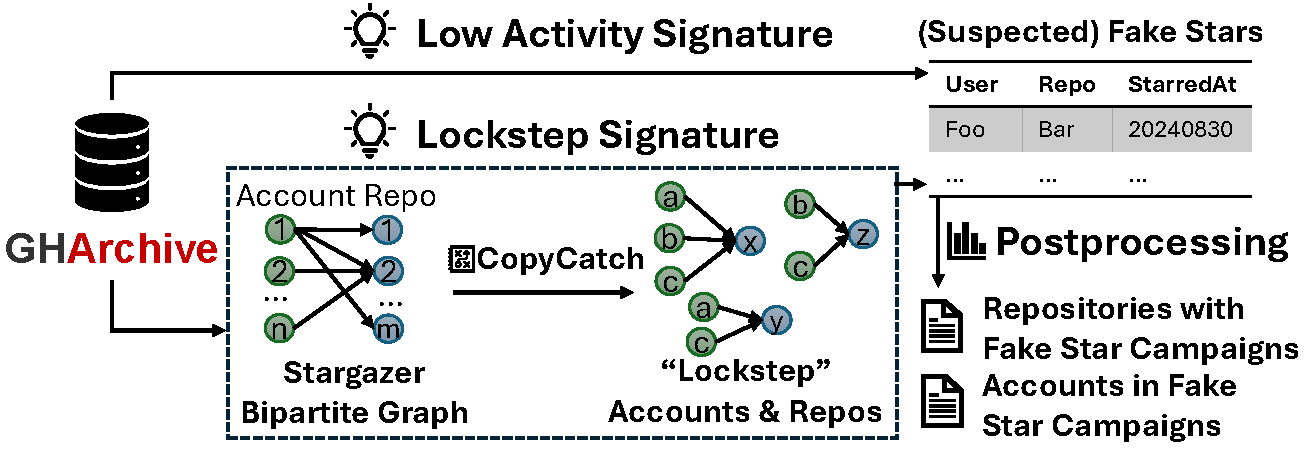
\includegraphics[width=\linewidth]{figs-fake-stars/ToolOverview.pdf}
    \caption{A high-level overview of \SystemName.}
    \label{fig:system-overview}
\end{figure}

\begin{figure}[t]
    \centering
    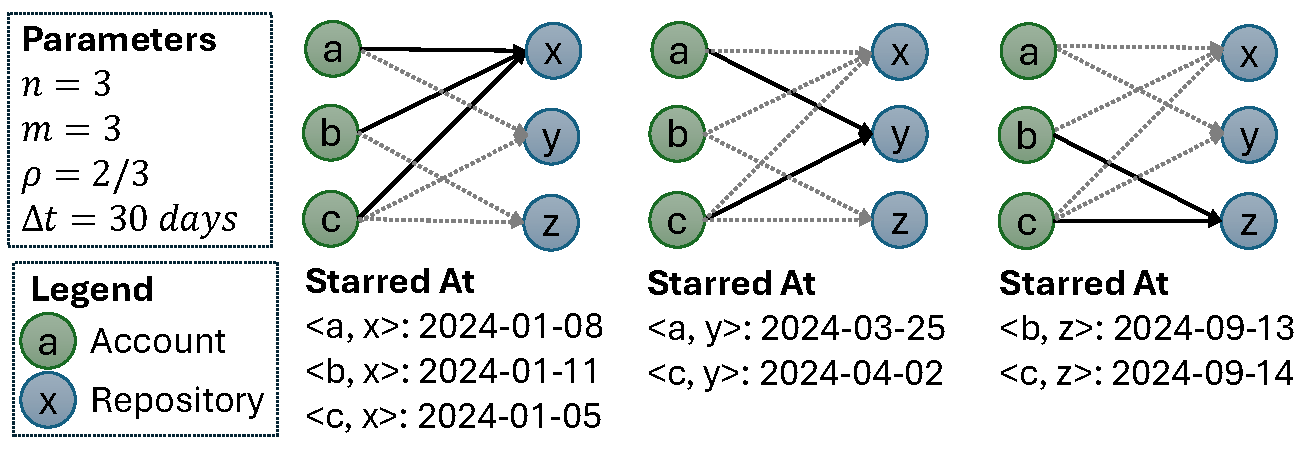
\includegraphics[width=0.97\linewidth]{figs-fake-stars/Example.pdf}
    \caption{Under the parameter setting shown above, accounts $a, b, c$ and repositories $x, y, z$ are considered to demonstrate a lockstep signature because each repository has stars from at least two of these accounts in a 30-day time window.}
    \label{fig:example}
\end{figure}

\subsection{Heuristics and Postprocessing}
\label{sec:approach}

\textbf{The Low Activity Signature.}
To detect the low activity signature, \SystemName finds GitHub accounts with only one \Code{WatchEvent} (i.e., have only starred one GitHub repository), plus at most one additional event (e.g., \Code{ForkEvent}) in the same repository on the same day.
This heuristic is inspired by a heuristic proposed in the gray literature~\cite{dagster}, but further simplified and tuned to avoid costly interactions with the rate-limited GitHub APIs and easy-to-obfuscate rules. % in their proposed heuristic.
While the detected accounts may be throw-away bot accounts controlled by fake star merchants, they may also be real users wrongly identified (e.g., someone legitimately registered an account, starred a repository, and then gave up using GitHub).
To partially address such cases, we also look at fake star counts at the repository level. 
That is, we only consider repositories with at least 50 stars suspected as fake, based on the observation that fake star merchants often sell a minimum of 50 stars (see Appendix, Section~\ref{sec:conclusion}).
Consequently, we ignore the fake stars (and corresponding users) in repositories with fewer than 50 fake stars in total.
We will also use this cutoff of 50 in the lockstep signature detector and the postprocessing step, based on the same intuition.

\textbf{The Lockstep Signature.}
If a fake star merchant controls a group of accounts to repeatedly deliver stars to repositories in their promised delivery time, it would create a unique ``lockstep'' signature.
Prior social network research shows that this signature is unlikely to form naturally and highly correlated to fraudulent activities~\cite{DBLP:conf/www/PanditCWF07, DBLP:conf/www/BeutelXGPF13, DBLP:conf/kdd/HooiSBSSF16}.
Mathematically speaking, let $\mathbf{U}$ be the set of all GitHub accounts and $\mathbf{R}$ be the set of all GitHub repositories; all GitHub stars effectively form a bipartite graph $\langle \mathbf{U}, \mathbf{R}, \mathbf{E} \subseteq \mathbf{U} \times \mathbf{R}, \tau: \mathbf{E}\mapsto \mathbf{T}\rangle$ where each $\langle u, r \rangle \in \mathbf{E} $ represents a star from account $u$ to repository $r$ and $\tau(\langle u, r \rangle)$ maps to the time of starring.
Given four parameters $\langle n, m, \rho, \Delta t\rangle$, we consider a group of accounts $U\subseteq\mathbf{U}$ and repositories $R\subseteq\mathbf{R}$ to demonstrate a \emph{lockstep signature} if:
\begin{align*}
|U| &\geq n, \quad |R| \geq m \\
\forall r \in R, \exists U_r \subseteq U, \exists t_r \in \mathbf{T}: \quad &|U_r| \geq \rho n,\\
&\forall u \in U_r: \langle u, r \rangle \in \mathbf{E},\\ 
&\forall u \in U_r: \tau(\langle u, r \rangle) \in [t_r, t_r + \Delta t]
\end{align*}
In other words,  we consider a group of accounts and repositories to be ``lockstepping'' if each repository has stars from at least $\rho n$ accounts in a time window no longer than $\Delta t$ (see Figure~\ref{fig:example} for an example). 
Note that this definition is both an extension and a relaxation of bicliques (or complete bipartite subgraphs)~\cite{DBLP:journals/dam/Peeters03}, as the latter are generally very rare in real large-scale bipartite graphs.

To find accounts and repositories with the lockstep signature at scale, \SystemName implements \textsf{CopyCatch}~\cite{DBLP:conf/www/BeutelXGPF13}, a state-of-the-art algorithm that has been deployed at Facebook to detect fake Likes with the same lockstep signatures.
At a high level, the algorithm starts from a set of seed repositories.
For each seed repository, it iteratively calibrates a time window and finds the largest possible group of accounts and repositories demonstrating a lockstep signature within that time window.
Finally, groups with more than $n$ accounts and $m$ repositories are retained and considered as engaging in suspicious fake starring activities.
We refer interested readers to the original paper~\cite{DBLP:conf/www/BeutelXGPF13} and our implementation (Section~\ref{sec:data-avail}) for the details of \textsf{CopyCatch}.
While the problem of finding maximum bicliques is NP-complete~\cite{DBLP:journals/dam/Peeters03} and \textsf{CopyCatch} is fundamentally a greedy local search algorithm, it is highly scalable and has been shown to work reasonably well in practice~\cite{DBLP:conf/www/BeutelXGPF13}.

\begin{comment}
\begin{figure}
    \centering
    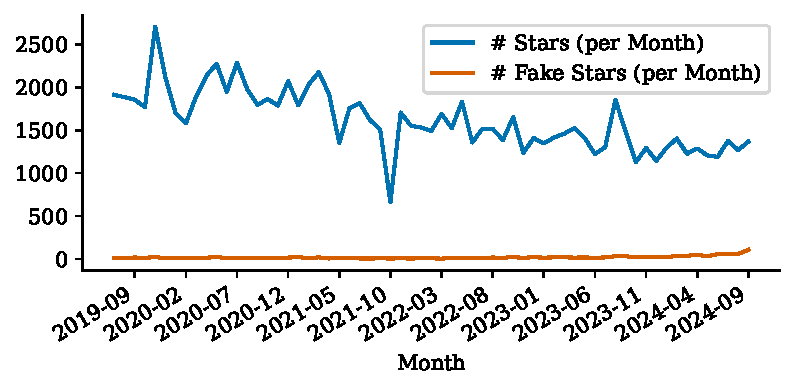
\includegraphics[width=\linewidth]{figs-fake-stars/vscode-timeline.pdf}
    \caption{The GitHub stargazer timeline of \href{https://github.com/microsoft/vscode}{\emph{microsoft/vscode}}. \SystemName reports 1,143 fake stars out of its $\sim$97k total stars, but they are scattered over time and barely have an effect on its number of stars received in each month.}
    \label{fig:postprocessing-example}
\end{figure}
\end{comment}

\textbf{Postprocessing.}
Even if the above two signatures identify significantly anomalous patterns in GitHub stargazer data, it is unreasonable to expect that every repository receiving fake stars is actively seeking fake stars. % (e.g., see Figure~\ref{fig:postprocessing-example}).
%As these fake stars do not appear meaningful in such a highly popular repository, 
In fact, we find that many highly popular repositories get a relatively small amount of fake stars; we infer that fake accounts deliberately star them as an adversarial behavior to evade platform detection.
Therefore, \emph{the postprocessing step aims to identify and keep only repositories with an anomalous spike of fake stars that contributes a non-negligible portion of stars obtained in that repository}.
We infer that these repositories have probably run a fake star campaign and are probably not a victim of fake stargazers, as they gained a noticeable benefit from those stars.
For this purpose, \SystemName aggregates monthly star counts to find repositories where (1) there is at least one single month in which it gets more than 50 fake stars and the percentage of fake stars exceeds 50\%;\footnote{The magic number 50 follows the same rationale as the low activity signature, that fake star merchants often sell a minimum of 50 stars (see Appendix, Section~\ref{sec:conclusion}).} (2) the all-time percentage of fake stars (relative to all stars) exceeds 10\%. %\footnote{While it seems tempting to use time series anomaly detection techniques~\cite{DBLP:journals/csur/Blazquez-Garcia21} to detect such anomalous spikes, most repositories in our data are extremely short-lived (Section~\ref{sec:rq2}), leading to very short time series unsuitable for most of these techniques.}
\SystemName considers these repositories as \emph{repositories with fake star campaigns} and the accounts that starred in these anomalous spike months as \emph{accounts in fake star campaigns}.

\subsection{Implementation}
\label{sec:implementation}

We implement detectors for the low activity signature and each iteration step of \textsf{CopyCatch} (for detecting the lockstep signature) as SQL queries on Google BigQuery, which enables \SystemName to scale the detection to all GitHub in a distributed manner.
We use Python scripts to dynamically generate and send these queries, and collect  fake stars from each query output into a local MongoDB database (using Google Cloud Storage as relay).
We set the lockstep signature parameters as: $n=50$, $m=10$, $\Delta t = 30\text{\emph{~days}}$, and $\rho = 0.5$; in other words, we seek to find clusters of $\ge$50 accounts and $\ge$10 repositories, such that there exists a 30-day interval for each repository in which it gets $\ge$25 stars from these accounts.
As the stargazer bipartite graph is extremely large (326 million edges from July 2019 to December 2024), we split the graph into interleaving six-month chunks (e.g., Jan - Jun 2024, Apr - Sept 2024).
The chunks are interleaved to avoid missing detections across chunk boundaries, and new chunks can be analyzed on a quarterly basis.

We initially deployed \SystemName in July 2024 when it scanned fake stars in the past five years, totaling more than 20 TB of data from \textsf{GHArchive}.
Then, we updated and merged two additional chunks with the latest cutoff of December 2024.
In total, \SystemName identified \textbf{six million (suspected) fake stars} across 26,254 repositories %created by 1.5 million accounts 
before the postprocessing step; %designed to remove spurious ones); 
among these stars, 1.06 million are identified with the low activity signature and 4.93 million with the lockstep signature.
In the postprocessing step, \SystemName identified 18,617 repositories with fake star campaigns and 301k participating accounts (corresponding to 3.81 million fake stars).

\subsection{Evaluation}
\label{sec:evaluation}

It is challenging to evaluate a fake activity detector like \SystemName.
While honeypots are often used in prior research (e.g., \cite{DBLP:conf/acsac/DuYZDWH0020, DBLP:conf/imc/CristofaroFJKS14, DBLP:journals/dss/CresciPPST15}), they raise ethical concerns~~\cite{DBLP:conf/icissp/WeipplSR16, DBLP:conf/uss/KohnoAL23}: If we were to buy fake stars for a honeypot repository, we would be effectively funding malicious actors and creating spam for other developers.
%Plus, there is no guarantee that fake stars from a few easy-to-find merchants would be representative---it was reported that attackers may use much more sophisticated methods to generate fake stars
%that need to be assessed in the specific research context~\cite{DBLP:conf/icissp/WeipplSR16, DBLP:conf/uss/KohnoAL23}
To alleviate this concern, we evaluate the recall of \SystemName using an alternative ground truth malware phishing campaign arguably powered by fake stars.
Specifically, we use the Stargazer Ghost Network dataset~\cite{stargazer-goblin}, which contains 847 repositories with more than 50 GitHub stars coming from 15,672 highly suspicious GitHub accounts. %(in that they have almost no seemingly legitimate activities other than starring suspicious repositories). %in which the attackers likely obstars are attacker generated fale stars %
%The accounts 
%where the attackers likely promoted their malware phishing repositories using fake GitHub stars.
We find that \SystemName can detect 688 (81.23\%) of the 847 repositories and 11,903 (75.95\%) of the 15,672 involved GitHub accounts.
\emph{In other words, \SystemName can achieve up to 82.23\% recall for repositories and 75.95\% recall for accounts when it comes to the detection of fake-star-powered malware campaigns.}
We believe this recall performance is satisfactory, especially considering that the algorithm we use for detecting the lockstep signature, \textsf{CopyCatch}, is a randomized greedy algorithm with no completeness guarantees~\cite{DBLP:conf/www/BeutelXGPF13}.

% While the above evaluation provides evidence regarding the \emph{recall} of \SystemName's detections, it does not provide any evidence regarding \emph{precision}.
Precision is inherently harder to evaluate because there is no obvious way to examine whether a star is fake or not.
Instead, we estimate \textit{criterion validity}~\cite{cohen1996psychological}, i.e., the extent to which an outcome is correlated to some other theoretically-relevant outcomes (or criterion).
In our case, we compare \emph{the percentage of GitHub repositories and accounts that have been deleted} (as of January 2025) between a comparison sample and the sample detected by \SystemName.
We choose this criterion based on reports of GitHub actively countering fraudulent and malicious activities~\cite{wired-news}---thus, we should be able to observe a higher deletion rate in the \SystemName sample compared to the baseline, especially if fake stars are also used for other malicious activities (like the Stargazer Ghost Network~\cite{stargazer-goblin}).
Therefore, for all repositories and 10,000 sample accounts (downsampled due to GitHub's API rate limit) found by \SystemName, we check (using the GitHub API) whether they were still accessible at the time of detection. %(Jul 2024, Oct 2024, or Jan 2025).
We also randomly sampled another 10,000 GitHub repositories with $\ge$50 stars and 10,000 GitHub stargazers in these repositories, to get baseline deletion percentages for comparison.
%Table~\ref{tab:evaluation} summarizes the results.

\begin{table}[t]
    \small
    \centering
    \caption{The fraction of repositories/accounts detected by \SystemName and deleted on GitHub at the time of detection is drastically higher compared to the baseline level obtained from random GitHub repositories and users.}
    \label{tab:evaluation}
    \begin{tabular}{lrr}
    \toprule
      & \multicolumn{2}{c}{\% Deleted}\\
    %\% Deleted 
    & w/o Postprocessing & w. Postprocessing\\
    \midrule
    \multicolumn{2}{l}{\textbf{Repositories} (Baseline: 5.03\%)} \\
    ~~Low Activity & 14.38\% & 79.36\%\\
    ~~Lockstep & 82.03\% & 90.70\%\\
    ~~\textbf{All} & \textbf{70.05\%} & \textbf{90.42}\%\\
    %\addlinespace
    \multicolumn{2}{l}{\textbf{Accounts} (Baseline: 3.54\%)} \\
    ~~Low Activity & 19.19\% & 72.29\%\\
    ~~Lockstep & 23.03\% & 48.83\% \\
    ~~\textbf{All} & \textbf{18.77\%} & \textbf{57.07\%} \\
    \bottomrule
    \end{tabular}
\end{table}

%Table~\ref{tab:evaluation} shows that, 
\emph{Compared with the baseline deletion ratio (5.03\% for repositories and 3.54\% for users), the deletion ratios for the detected repositories and accounts are substantially higher} (Table~\ref{tab:evaluation}): 90.42\% of repositories and 57.07\% of accounts in fake star campaigns (i.e., with postprocessing in Table~\ref{tab:evaluation}) have been deleted. 
The percentage is lower if we consider all repositories and accounts with fake stars (i.e., without postprocessing in Table~\ref{tab:evaluation}), especially for those detected by the low activity signature, providing support for the effectiveness and necessity of the postprocessing step.
Overall, the results align with our intuition that both signatures may be noisy in identifying individual fake stars but, when combined, effective in identifying repositories with fake star campaigns. 
The deletion ratio of accounts is generally lower than that of repositories, which can be interpreted in multiple ways. For example, it may be that \SystemName is less accurate at identifying sophisticated fake accounts (e.g., those detected by the lockstep signature); it is also possible that GitHub prioritizes taking down malware/phishing repositories, as supported by our RQ3 results (Section~\ref{sec:rq3}).

\subsection{Limitations and Ethical Concerns}
\label{sec:limitations}

The most important limitation of \SystemName is that, while it detects statistically anomalous starring patterns in GitHub, the evidence from \SystemName alone is insufficient for disciplinary action (e.g., for taking down fraudulent repositories and accounts).
The latter would usually require evidence from non-public information (e.g., IP addresses).
In general, it is possible that some of the \SystemName identified repositories and accounts may still be false positives.
Another limitation of \SystemName is the use of ad-hoc heuristics and parameters (notably the 50 stars threshold in many parts of detection).
While it is challenging to run thorough sensitivity tests on these parameters due to the sheer amount of data to be processed, we used our best judgment in choosing these parameters.
Also, considering the generally high face validity of our evaluation and measurement study results (Section~\ref{sec:evaluation} and Section~\ref{sec:measurement-study}), we believe the performance of \SystemName suffices for our research goal---characterizing the landscape of an emerging threat.

The possibility of false positives in \SystemName detections also brings ethical concerns.
Even if \SystemName is $\sim$99\% precise in detecting repositories that bought fake stars, there would still be $\sim$180 false positive repositories in our resulting dataset, and interpreting them as having done so would potentially harm their reputation.
To mitigate such risks, we focus on presenting statistical patterns and avoid giving individual repositories as examples in the paper (unless they are obviously malicious).
We also carefully discussed and noted ethical concerns in the dataset documentation, calling for its responsible use and interpretation  (Section~\ref{sec:conclusion}).


\section{Measurement Study}
\label{sec:measurement-study}

Using the dataset of 18,617 repositories and 301k accounts with fake star campaigns (Section~\ref{sec:implementation}), we conduct a measurement study of fraudulent starring activities in GitHub, that answers the following four research questions (formulated in Section~\ref{sec:introduction}):
\begin{itemize}[leftmargin=15pt]
    \item \RQOne
    \item \RQTwo
    \item \RQThree
    \item \RQFour
\end{itemize}
The first three research questions involve different angles of exploratory analysis of this dataset.
The final research question aims to quantify the impact of fake star campaigns: Are they really effective in attracting more (legitimate) attention just as real stars, or only effective in making repositories seem momentarily popular?

\subsection{RQ1: Prevalence}
\label{sec:rq1}

\textbf{Motivation.} 
While \SystemName has detected an enormous number of repositories and accounts with fake star campaigns, it is not yet clear to what extent these repositories and accounts may affect open-source software development and the software supply chain as a whole.
To understand this, we need to provide evidence on: (a)~the prevalence of fake stars and involved repositories \& accounts relative to regular GitHub activities; (b)~the prevalence of fake-star-related repositories in popular distribution channels (e.g., GitHub Trending~\cite{github-trending} and package registries such as npm and PyPI).

\textbf{Prevalence w.r.t. Overall GitHub Activity.}
For each month in our observation period (July 2019 to December 2024), we compute the following: (a)~the percentage of fake GitHub stars among all GitHub stars in that month; (b)~the percentage of GitHub accounts in fake star campaigns, among all active GitHub users (i.e., at least one \textsf{GHArchive} event) in that month; (c)~the percentage of GitHub repositories with fake star campaigns among all repositories that received $\ge 50$ stars in that month.
Through this operationalization, we can estimate the portion of GitHub activities that may have been faked and the impact of these faked activities.
% (as measured by the percentage of repositories with fake star campaigns among all repositories gaining $\ge$50 stars in that month).

\begin{figure}
    \centering
    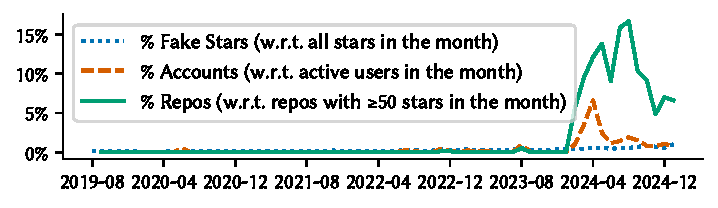
\includegraphics[width=\linewidth]{figs-fake-stars/ts_percentage.pdf}
    %\vspace{-1mm}
    \caption{The percentage (\%) of GitHub stars, accounts, and repositories involved in fake star campaigns in each month.}
    %\vspace{-2mm}
    \label{fig:prevalence}
\end{figure}

\begin{figure}
    \centering
    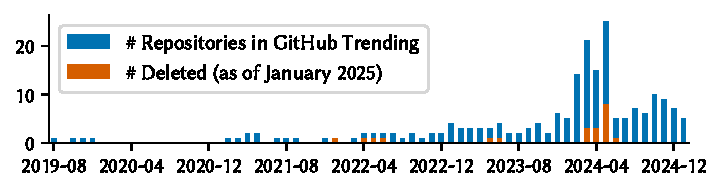
\includegraphics[width=\linewidth]{figs-fake-stars/ts_trending.pdf}
    %\vspace{-1mm}
    \caption{The number (\#) of GitHub repositories with fake star campaigns and appeared in GitHub Trending each month.}
    \label{fig:trending}
\end{figure}

We observe in Figure~\ref{fig:prevalence} that fake stars still only constitute a small fraction ($\le$1\%) of all GitHub stars each month, but fake star campaigns have been increasing since 2022 and surged since 2024.
Their broadest impact was in July 2024, when 16.66\% of popular repositories (3,499) had fake star campaigns. 
March 2024 sees the highest percentage of fake star accounts (6.59\%, 117,024).

\begin{summary-rq}
\textbf{Finding 1:} Fraudulent starring activities started to gain momentum in 2022 and have surged in 2024.
\end{summary-rq}

\textbf{Prevalence in GitHub Trending.}
While the above analysis provides evidence regarding the general prevalence of repositories with fake star campaigns, it is still unclear whether these repositories actually reach developers.
To study this, we pull historical records of GitHub Trending~\cite{github-trending} repositories from a community-maintained archive~\cite{trending-archive}.
Note that this archive only collects trending repositories from five programming languages (Python, Go, C++, JavaScript, and CoffeeScript), so we likely underestimate the actual reach of the studied repositories in GitHub Trending.
In total, we identified 78 (0.42\%) repositories with fake star campaigns that have also appeared in GitHub Trending.
While we also see a similar 2024 surge (Figure~\ref{fig:trending}), the peak number is only 25 (in March 2024).
This lower reach, compared with the results in Figure~\ref{fig:prevalence}, suggests that the GitHub trending algorithm is effective at filtering out most superficially-popular repositories.
Among the matched subset, we anecdotally note repository names suggestive of malicious activities, e.g., \Code{Wallet-stealer} and \Code{blooket-hacks}; we will further analyze these repositories in Section~\ref{sec:rq3}.

\begin{summary-rq}
\textbf{Finding 2:} 
Only a small number (78; 0.42\%) of repositories with fake star campaigns reached the GitHub Trending page.
\end{summary-rq}

\textbf{Prevalence in Package Registries.}
To identify the prevalence of repositories with fake star campaigns in existing package registries, we use the \textsf{ecosyste.ms} API~\cite{ecosystems} to query for explicit references to the GitHub repositories in our dataset.\footnote{This result is also an undercount, as explicit links to GitHub are optional.} % over 63 package registries.
We matched 738 packages (corresponding to 229 repositories); the most common registries are: PyPI (159 packages), npm (145), Pub (138), Cargo (123), and Go (118).
We further collected their adoption statistics (i.e., \# of dependent packages within the registry and \# of dependent repositories in GitHub).
Overall, results (Table~\ref{tab:downloads}) show scarce
evidence of actual adoption for most of these packages despite their inflated star counts: 70.46\%/77.50\% of these packages do not even have a single dependent open-source package/repository, respectively.

\begin{table}
    \small
    \centering
    \setlength{\tabcolsep}{4pt}
    \caption{Descriptive statistics for the 738 packages linked to 229 repositories with fake star campaigns.}
    \begin{tabular}{lrrrrrrr}
    \toprule
         &  mean & min & 25\% & 50\% & 75\% & max \\
    \midrule
         \# stars & 1686.69 & 54 & 240 & 380 & 1235 & 29.06k\\
         %\# releases & 37.35 & 0 & 1 & 7 & 36 & 836 \\
         %\# downloads & 26.79k & 0 & 70 & 947 & 13.34k & 442.2k \\
         \# dependent packages & 1.69 & 0 & 0 & 0 & 1 & 149 \\
         \# dependent GitHub repos & 5.26 & 0 & 0 & 0 & 0 & 677\\
    \bottomrule
    \end{tabular}
    \label{tab:downloads}
\end{table}

\begin{summary-rq}
\textbf{Finding 3:} 
Only a small number (229; 1.23\%) of repositories with fake star campaigns are also published in package registries (totaling 738 packages). Even fewer are widely adopted.
\end{summary-rq}

\subsection{RQ2: Activity Patterns}
\label{sec:rq2}

\textbf{Motivation.}
While \SystemName detects anomalous starring patterns by construction (Section~\ref{sec:approach}), it does not look into other types of GitHub activities.
Understanding the latter may offer insights into how fake star campaigns operate and what they are used for.
In this RQ, we examine the activity patterns of repositories and accounts with fake star campaigns from two different angles: (a) their overall duration of activity and (b) the distribution of activity types.

\begin{figure}
\centering

\begin{subfigure}{0.49\linewidth}
    \centering
    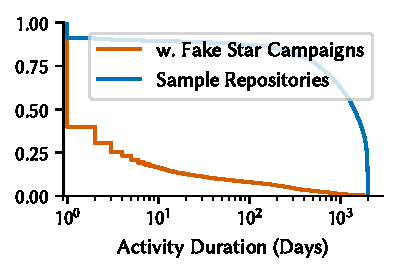
\includegraphics[width=\linewidth]{figs-fake-stars/survival_repo.pdf}
    \caption{Repositories}
    \label{fig:survival-repos}
\end{subfigure}
\begin{subfigure}{0.49\linewidth}
    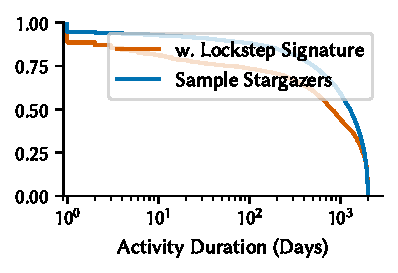
\includegraphics[width=\linewidth]{figs-fake-stars/survival_user.pdf}
    \caption{Accounts}
    \label{fig:survival-actors}
\end{subfigure}
\vspace{-1mm}
\caption{The Complementary Cumulative Distribution Function (CCDF) of activity durations for (a) repositories with fake star campaigns and sample repositories, (b) accounts with the lockstep signature and sample stargazers.}
\vspace{-1mm}
\label{fig:survival}
\end{figure}

\textbf{Duration of Activity.}
For repositories and accounts with fake star campaigns, we define their activity duration as the number of days from their first \textsf{GHArchive} event to their last. %\textsf{GHArchive} event.
Since accounts with the low-activity signature (31.99\% of accounts in fake star campaigns) have one day of activity by construction, we focus on the activity duration of accounts with the lockstep signature.
For these latter accounts, we compare the Complementary Cumulative Distribution Function (CCDF) of their activity durations with the same comparison samples we used in Section~\ref{sec:evaluation} (Figure~\ref{fig:survival}).
We observe that most repositories with fake star campaigns are short-lived (Figure~\ref{fig:survival-repos}): 83.90\% of repositories with fake star campaigns have less than ten days of activity.
However, user accounts with the lockstep signature can be active for long, with the overall distribution being similar to average GitHub stargazers (Figure~\ref{fig:survival-actors}).

\begin{summary-rq}
\textbf{Finding 4:} 
Most repositories with fake star campaigns are short-lived, but accounts can stay active for a long time. 
\end{summary-rq}

\begin{figure}
\centering
\begin{subfigure}{0.49\linewidth}
    \centering
    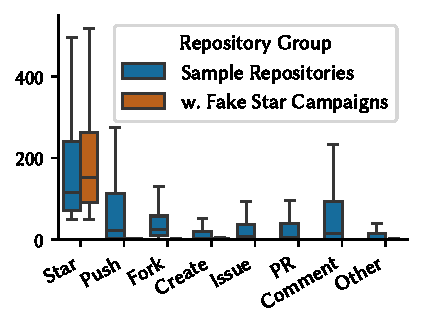
\includegraphics[width=\linewidth]{figs-fake-stars/repo-events.pdf}
    \caption{
    Repositories
    %The distribution of the number of events \emph{per repository}
    }
    \label{fig:repo-events}
\end{subfigure}
\begin{subfigure}{0.49\linewidth}
    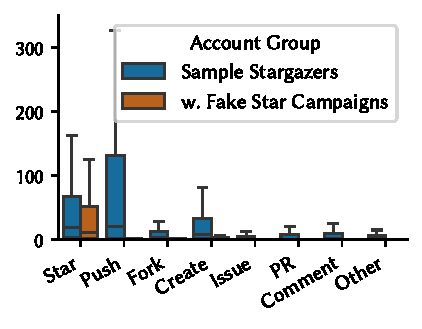
\includegraphics[width=\linewidth]{figs-fake-stars/actor-events.pdf}
    \caption{
    Accounts
    %The distribution of the number of events \emph{per account}
    }
    \label{fig:actor-events}
\end{subfigure}
\vspace{-1mm}
\caption{Comparing the distribution of GitHub events between: (1) repositories and accounts with fake star campaigns, and (2) random samples of repository and stargazers.}
\vspace{-1mm}
\label{fig:events}
\end{figure}

\textbf{Distribution of Activity Types.}
We aggregate the \textsf{GHArchive} events of repositories and accounts with fake star campaigns into eight types: \emph{Star}, \emph{Push}, \emph{Fork}, \emph{Create}, \emph{Issue}, \emph{PR} (i.e., pull requests), \emph{Comment}, and \emph{Other}.
Then, we compare the overall distributions of activity types with the same samples we used in Section~\ref{sec:evaluation}, aggregating the results in Figure~\ref{fig:events}.
We can observe that repositories and accounts in fake star campaigns tend to be skewed toward starring activities, and they rarely engage in activities that are considerably harder to fake (e.g., issues, pull requests, comments).

However, some repositories and accounts may have different patterns compared to the trends in Figure~\ref{fig:events}. 
To explore this, we run the $k$-Means algorithm~\cite{DBLP:conf/soda/ArthurV07} under different $k$s on normalized activity vectors from repositories and accounts, respectively.
We did not find meaningful clusters for repositories, but we find two additional clusters for accounts: Table~\ref{tab:cluster-center} shows cluster centers for $k = 3$, which has the highest Silhouette Coefficient~\cite{rousseeuw1987silhouettes} among $k \in [2,8]$.
Apart from the majority of accounts that almost exclusively star repositories (Cluster 0, 77.75\%), we find a cluster (Cluster 1, 14.76\%) in which the accounts look generally more realistic---with pushes, repository creations, and other activities.
Our manual analysis of a sample in Cluster 1 indicates that some of them may be creating and pushing artificial repositories to evade platform moderation, but there are also cases where we cannot tell whether they are real or not from their GitHub profiles.
Finally, a small portion of accounts (Cluster 2, 7.49\%) tend to engage in both starring and forking activities; we believe they may come from merchants selling both stars and forks.

\begin{table}
    \centering
    \small
    %\setlength{\tabcolsep}{3.5pt}
    \caption{The properties of each clustering center identified by $k$-Means on accounts in fake star campaigns.}
    \vspace{-1mm}
    \begin{tabular}{lrrrrrr}
    \toprule
        & \% Star & \% Push & \% Fork & \% Create & \% Other \\
    \midrule
        Cluster 0 (77.75\%) & 95.56\% & 1.00\% &  0.69\% & 2.10\% & 0.65\% \\
        Cluster 1 (14.76\%) & 28.55\% & 40.44\% & 2.55\% & 17.94\% & 10.52\% \\
        Cluster 2 (7.49\%) & 52.34\% & 1.08\% & 43.74\% & 1.76\% & 1.08\%\\
    \bottomrule
    \end{tabular}
    \label{tab:cluster-center}
\end{table}

\begin{summary-rq}
\textbf{Finding 5:} 
Most repositories and accounts with fake star campaigns have trivial GitHub activity patterns.
\end{summary-rq}


\begin{comment}
\begin{table}
    \centering
    \setlength{\tabcolsep}{6pt}
    \caption{The percentage of accounts with default avatar, no GitHub organization, no company affiliations, and no personal websites in three groups: fake accounts reported by Du et al.~\cite{DBLP:conf/acsac/DuYZDWH0020}, accounts in our detected fake star campaigns, and a sample of random GitHub stargazers (Section~\ref{sec:evaluation}).}
    \begin{tabular}{lrrr}
    \toprule
         & Du et al.~\cite{DBLP:conf/acsac/DuYZDWH0020} & w. Campaigns & Sample Users\\
    \midrule
       Default Avatar & 21.76\% & 50.25\% & 38.76\%\\
       No Organization & 85.42\% & 95.78\% & 92.45\%\\
       No Affiliations & 71.90\% & 88.49\% & 79.62\%\\
       No Website & 64.81\% & 80.69\% & 79.31\%\\
    \bottomrule
    \end{tabular}
    \label{tab:user-stat}
\end{table}

For this research question, our exploration starts with comparing the profile characteristics of the GitHub accounts participating in fake star campaigns with the baseline sample of accounts we obtained in Section~\ref{sec:evaluation} and with the results reported in the literature~\cite{DBLP:conf/acsac/DuYZDWH0020}.
Therefore, we collect and summarize the same four profile characteristics also analyzed by Du et al.~\cite{DBLP:conf/acsac/DuYZDWH0020} and summarize the results in Table~\ref{tab:user-stat}.
Compared with the fake accounts found through a honeypot repository by Du et al.~\cite{DBLP:conf/acsac/DuYZDWH0020}, the accounts in our fake star campaign dataset are overall more likely to have a default avatar, do not belong to an organization on GitHub, and state no affiliation or website in their profile.
It is possible that fake star merchants in Du et al.~\cite{DBLP:conf/acsac/DuYZDWH0020}'s dataset may have different account management and creation strategies compared to merchants as of now.
However, while users in fake star campaigns are slightly more likely to have these empty fields, the differences compared with random GitHub stargazers are not large, especially considering how drastically different their activity patterns are (Figure~\ref{fig:actor-events}).
This indicates that judging a user's profile information by how realistic it appears is not a useful indicator of whether the user participates in fake star campaigns.


\begin{summary-rq}
\textbf{Finding 6:} 
Compared to average GitHub users, accounts in fake star campaigns are slightly more likely to have an empty profile, but the differences are relatively small.
\end{summary-rq}

\begin{table}
    \centering
    \setlength{\tabcolsep}{5pt}
    \caption{Descriptive statistics for repositories with fake star campaigns (deleted vs. still on GitHub).}
    \begin{tabular}{lrrrrrrr}
    \toprule
         &  mean & min & 25\% & 50\% & 75\% & max \\
    \midrule
    \multicolumn{3}{l}{\textbf{deleted ($n = 14,371$)}} \\
    \# stars (total) & 203 & 50 & 88 & 139 & 247 & 6.82k \\
    \# stars (suspected fakes) & 193 & 50 & 83 & 129 & 236 & 4.39k \\
    \# month w. campaign & 1.01 & 1 & 1 & 1 & 1 & 3 \\
    \# days active & 19.0 & 1 & 1 & 1 & 3 & 1.74k \\
    \addlinespace
    \multicolumn{3}{l}{\textbf{Still on GitHub ($n = 1,464$)}} \\
    \# stars (total) & 358 & 50 & 102 & 171 & 286 & 25.3k \\
    \# stars (suspected fakes) & 206 & 50 & 80 & 112 & 179 & 11.3k \\
    \# stars (latest) & 331 & 0 & 18 & 96 & 284 & 27.1k \\
    \# month w. campaign & 1.08 & 1 & 1 & 1 & 1 & 6 \\
    \# days active & 359 & 1 & 45 & 195 & 506 & 1.92k\\
    \bottomrule
    \end{tabular}
    \label{tab:repositories}
\end{table}
\end{comment}

\subsection{RQ3: Repository Characteristics}
\label{sec:rq3}

\textbf{Motivation.}
While RQ1 and RQ2 provide statistics on the detected repositories and accounts with fake star campaigns, they do not provide evidence regarding \emph{what exactly these repositories are}.
The anecdotes from the gray literature
% often suggests (from a few examples) 
suggest that repositories may buy fake stars for popularity contests, growth hacking, or convincing investors~\cite{startup-stars, wired-news}; malicious actors may orchestrate fake star campaigns to spread malware phishing repositories~\cite{stargazer-goblin}.
Can we confirm these reports on \SystemName's detections at a larger scale?
What are the most common domains where fake star campaigns occur?
We answer these subquestions in RQ3.

\begin{table}[t]
    \small
    \centering
    \caption{The most common words in the names of deleted repositories with fake star campaigns.}
    \label{tab:common-words}
    \begin{tabular}{lp{6cm}}
    \toprule
        Category & Words and Occurrences \\
    \midrule
        Pirated software & free (856), crack (721), pro (656), adobe (618), activation (467), cracked (263), studio (239), photoshop (177) \\
        Cryptocurrency & bot (1,071), autoclicker (438), executor (321), crypto (312), wallet (241), trading (175), solana (154)\\ 
        Game cheats & hack (357), cheat (256), roblox (252), h4ck (196)\\
    \bottomrule
    \end{tabular}

\end{table}


\begin{table}[t]
    \small
    \setlength{\tabcolsep}{4.5pt}
    \centering
    \caption{We categorize different groups of repositories with fake star campaigns (trending, packages, and others) into nine categories. Their frequencies are as follows.}
    \begin{tabular}{lrrrr}
    \toprule
       Category & Trending & Packages & Other & All  \\
    \midrule
        \textsf{Spam/Phishing} & 16 (20.5\%) & 22 (9.6\%) & 93 (31.1\%) & 131 (22.6\%)\\
        \textsf{AI/LLM} & 25 (32.1\%) & 36 (15.7\%) & 45 (15.1\%) & 96 (16.6\%)\\
        \textsf{Blockchain} & 10 (12.8\%) & 44 (19.2\%) & 30 (10.0\%) & 76 (13.1\%) \\
        \textsf{Tool/Application} & 15 (19.2\%) & 22 (9.6\%) & 39 (13.0\%) & 73 (12.6\%)\\
        \textsf{Tutorial/Demo} & 4 (5.1\%) & 6 (2.6\%) & 61 (20.4\%) &  70 (12.1\%)\\
        \textsf{Web Frameworks} & 5 (6.4\%) & 44 (19.2\%) & 9 (3.0\%) & 56 (9.7\%) \\
        \textsf{Basic Utility} & 0 (0.0\%) & 27 (11.8\%) & 3 (1.0\%) & 30 (5.2\%) \\
        \textsf{Database} & 0 (0.0\%) & 10 (4.4\%) & 4 (1.3\%) & 14 (2.4\%)\\
        \textsf{Other} & 3 (3.8\%) & 17 (7.4\%) & 15 (5.0\%) & 34 (5.9\%) \\ 
    \bottomrule
    \end{tabular}
    \label{tab:repo-labels}
\end{table}


\textbf{Analysis of Deleted Repositories.}
Our first analysis focuses on the 90.42\% of repositories that have already been deleted on GitHub. 
Unfortunately, it is very difficult to study these repositories: They become inaccessible immediately after deletion from GitHub and \textsf{GHArchive} does not store any repository content.\footnote{
World of Code~\cite{DBLP:journals/ese/MaDBAVTKZM21} (WoC), another possible source of repository data, contains only a small portion of these deleted repositories---we believe they are likely unrepresentative of the remaining ones, depending on the specific discovery mechanisms used in WoC.
% As a side note, we were only able to recover less than 1\% of these deleted repositories from World of Code~\cite{DBLP:journals/ese/MaDBAVTKZM21}.
% We believe they are likely not representative of the remaining unrecoverable ones---a repository probably needs much more activities than the average repository in our dataset (RQ2), to be discovered and archived by World of Code.
}
Despite this, we can still glean some information from a term frequency analysis of their \emph{repository names} (Table~\ref{tab:common-words}). 
We find that most of the deleted repositories carry names indicating pirated software (e.g., \Code{Adobe-Animate-Crack}), cryptocurrency bots (e.g., \Code{pixel-wallet-bot-free}, \Code{Solana-Sniper-Bot}), or game cheats (e.g., \Code{GTA5-cheat}).
While GitHub may have taken some of them down due to copyright violations, it is probably not the majority case: The gray literature shows that fake star campaigns are used to promote phishing malware repositories~\cite{stargazer-goblin}. %banshee, game-engine}.
Combining with the evidence we obtained from non-deleted repositories sharing similar names with deleted ones (e.g., Figure~\ref{fig:malware-example}, more examples in Appendix, Section~\ref{sec:conclusion}),
%\Code{Phantom-Sniper-Solana} for the repository in Figure~\ref{fig:malware-example}
we infer that most of these repositories could be phishing malware repositories masquerading as pirated software, game cheats, and cryptocurrency bots.

\begin{summary-rq}
\textbf{Finding 6:}
Most (90.42\%) repositories with fake star campaigns have been deleted on GitHub. 
Existing evidence suggests that they are probably phishing malware repositories masquerading as pirated software, game cheats, and cryptocurrency bots.
\end{summary-rq}

\textbf{Analysis of Non-Deleted Repositories.}
For the remaining non-deleted repositories (1,783 in total), we clone them immediately at the time of identification. 
Then, we conduct open coding~\cite{khandkar2009open} on the repository READMEs---referring to other files where necessary---on three groups of repositories:
(a) the 78 repositories that appeared in GitHub Trending (Section~\ref{sec:rq1}), which clearly reaches a wide range of developers;
(b) the 229 repositories that are linked by open-source packages (Section~\ref{sec:rq1}), which may have different characteristics compared to others;
(c) 299 randomly sampled repositories from the remaining 1,476 repositories (sample size determined from 95\% confidence level and 5\% margin of error).
From this analysis, we identify eight major categories of repositories (Table~\ref{tab:repo-labels}).
Among them, the most common---and also most concerning---category, is \textsf{Spam/Phishing} (31.1\% in Other, 22.6\% in All), where the repository is either an obvious clickbait (e.g., claiming game cheats, pirated software, cryptocurrency bots) to trick download of suspicious files or spreading spam content (e.g.,  used for search-engine-optimizations).\footnote{Note that while we try our best to identify spam/phishing repositories, it is still possible that we miss better-obfuscated malicious repositories and mis-categorize them into other categories.
We will discuss more on this limitation in Section~\ref{sec:discussion}.}
The remaining popular categories include: (1) \textsf{AI/LLM}, many of which are academic paper repositories or LLM-related startup products, (2) \textsf{Blockchain} or cryptocurrency related repositories, (3) \textsf{Tool/Applications}, or (4) \textsf{Tutorials/Demos} that seem to serve a reference or demonstration purpose (e.g., Python coding examples or list of awesome LLM tools).
We provide definition of each category, analysis of inter-rater reliability, and examples of \textsf{Spam/Phishing} repositories in Appendix (Section~\ref{sec:conclusion}).

\begin{summary-rq}
\textbf{Finding 7:} 
A significant portion ($\sim$30\%) of repositories with fake star campaigns, that are still accessible on GitHub at the time of writing (i.e., March 2025), are spam or active phishing malware repositories. 
The remaining ones are mostly AI/LLM, blockchain, tool/applications, or tutorial/demo repositories.
\end{summary-rq}

\subsection{RQ4: Promotional Effect}
\label{sec:rq4}

\textbf{Motivation.}
For the first three research questions, we have presented a set of exploratory results around the prevalence of fake stars and the characteristics of repositories and accounts with fake star campaigns.
While our RQ3 results highlight that the majority of repositories with fake star campaigns are likely short-lived phishing/spam repositories, there are still a non-negligible number of repositories in our dataset that remain online longer and seem more legitimate.
Why would they buy fake GitHub stars?
The gray literature often argues that (non-malicious) GitHub repositories buy fake stars for growth hacking~\cite{bohnsack2019hack}
(i.e., ``fake it until you make it''), especially because the number of stars is often considered a key indicator of the success of open-source projects and the occasional start-up companies associated with them~\cite{startup-stars}.
%reddit-discussion1, reddit-discussion2, hackernews-discussion1, hackernews-discussion2, startup-stars}.
Motivated by these speculations, we empirically analyze whether buying fake stars is effective in attracting substantial additional \emph{real} attention, or only effective in making the repositories momentarily seem a little more popular (by the amount of stars they buy).

\textbf{Hypotheses.}
We formulate the following two hypotheses regarding the effect of (fake and real) GitHub stars:
\begin{itemize}[leftmargin=15pt]
    \item \textbf{H$_1$:} \emph{Accumulating real GitHub stars will help a GitHub repository gain more real GitHub stars in the future.}
    \item \textbf{H$_2$:} \emph{Accumulating fake GitHub stars will help a GitHub repository gain more real GitHub stars in the future, but the effect is not as strong as that of real stars.}
\end{itemize}
We formulate \textbf{H$_1$} based on the well-known ``rich get richer'' phenomenon confirmed repeatedly in online social media and similar online contexts~\cite{DBLP:journals/corr/ZhuL16, hagar2022concentration}.
We formulate \textbf{H$_2$} because there is no straightforward way for a GitHub user to distinguish fake stars from real ones while browsing a repository's web page (indeed, we had to build and run a tool for this), and thus fake stars should have a similar effect as real stars for most users.
However, some users may look for other signals (e.g., issues and pull requests) and decide not to star the repository if other signals indicate poor quality, so we expect the effect to be smaller compared to real stars.

\textbf{Methodology.}
To test our hypotheses, we fit \emph{panel autoregression} models~\cite{hanck2021introduction}, estimating the longitudinal effect of gaining fake stars on attracting real stars in the future.
Panel autoregression models are a family of regression models tailored to work on panel data (e.g., variables are collected per repository in a series of time periods) with temporal dependencies (i.e., variables at time $t$ may be affected by variables at time $t - \Delta t$).
By adding fixed effect or random effect terms to the model (we report on both specifications below, to demonstrate that our results are robust), we will be able to estimate the longitudinal effect of independent variables robustly to unobserved heterogeneity (i.e., factors that may affect the outcome variable but are not measured in the model).
Specifically, %in our panel data, 
we collect the following variables for each repository $i$ in each month $t$: % when they were active:
\begin{itemize}[leftmargin=10pt]
    \item $\textit{fake}_{i,t}$: Count of fake stars repository $i$ gained in month $t$;
    \item $\textit{all\_fake}_{i,t}$:  Total count of fake stars in repository $i$ as of $t$;
    \item $\textit{real}_{i,t}$: Count of non-fake stars repository $i$ gained in month $t$;
    \item $\textit{all\_real}_{i,t}$: Total count of non-fake stars in repository $i$ as of $t$;
    \item $\textit{age}_{i,t}$: Number of months since repository $i$ creation;
    \item $\textit{release}_{i,t}$: Whether repository $i$ has at least one GitHub release before or during month $t$;
    \item $\textit{activity}_{i,t}$: The number of \textsf{GHArchive} events for repository $i$ in month $t$, that come from GitHub users who are not the repository owner or one of the fake stargazers. This is a proxy measure for the amount of authentic development activities in month $t$. 
\end{itemize}
The first four variables are intended to test our hypotheses; the remaining three are control variables that have been shown to correlate with star increases in prior work~\cite{DBLP:conf/icse/FangLHV22}. 
We fit $AR(k)$ (i.e., $k$-th order) models for $k = 1, 2, ..., 6$, defined as follows:
\begin{align*}
    \textit{real}_{i,t} \sim &\sum_{j=1}^k \textit{real}_{i, t-k} + \textit{all\_real}_{i, t - k - 1} + \sum_{j=1}^k \textit{fake}_{i, t-k} \\& + \textit{all\_fake}_{i, t - k - 1} + \textit{age}_{i,t} + \textit{release}_{i,t} + \textit{activity}_{i,t}\\
\end{align*}
The last three control variables are for random effect models only; unobserved heterogeneity in fixed effect models is controlled by the per-time and per-repository %invariant
fixed-effect terms.
All variables with skewed distributions are log-transformed before they are fed into the model.
We fit the models using the R \Code{plm} package~\cite{r-plm}.

\textbf{Limitations.}
Before diving into the modeling results, we note the inherent limitations of our modeling approach.
First, even if it allows for robust estimates of coefficients to represent the effect of independent variables, a regression model like ours may still provide insufficient evidence for causality claims.
While Granger causality tests are often used in the econometric literature to establish stronger evidence of causality~\cite{dumitrescu2012testing}, the majority of time series in our data are too short to fulfill the minimum requirements of Granger causality tests on unbalanced panels ($t \ge 6+2k$, $k$ is the autoregression order).
More importantly, it is possible that real causality hides in exogenous variables~\cite{engle1983exogeneity} (e.g., if the repository maintainer is technically inexperienced and shortsighted, that may both cause the maintainer to buy fake stars and the repository to gain fewer real stars).
Therefore, while our results provide initial evidence on the effect of fake stars on GitHub, future work is necessary to establish stronger evidence of causality and further uncover the mechanisms behind such effects.

\begin{table}
    \small
    \centering
    \caption{Fixed/random effect panel autoregression results.}
    \begin{tabular}{lrr} 
    \toprule
     & \multicolumn{2}{c}{\textit{Dependent Variable: $real_{i,t}$}} \\
     %\addlinespace
     & Random Effect & Fixed Effect \\
    \midrule 
     $\textit{real}_{i, t - 1}$ & 0.496$^{***}$ (0.015) & 0.364$^{***}$  (0.018)\\ 
     $\textit{real}_{i, t - 2}$ & 0.187$^{***}$ (0.014) & 0.148$^{***}$  (0.015)\\ 
     $\textit{all\_real}_{i, t - 3}$ & 0.069$^{***}$ (0.008) & 0.097$^{***}$ (0.021)\\ 
     $\textit{fake}_{i, t - 1}$ & 0.058$^{***}$ (0.011) & 0.074$^{***}$ (0.012) \\ 
     $\textit{fake}_{i, t -  2}$ & 0.024$^{**\textcolor{white}{*}}$ (0.010) & 0.029$^{**\textcolor{white}{*}}$ (0.011) \\ 
     $\textit{all\_fake}_{i, t - 3}$ & $-$0.026$^{***}$ (0.006) & $-$0.045$^{***}$ (0.014) \\ 
     $\textit{age}_{i,t}$ & $-$0.004$^{***}$ (0.001)  &  \\ 
     $\textit{release}_{i,t}$ & 0.084$^{***}$  (0.022) &  \\ 
     $\textit{activity}_{i,t}$ & 0.087$^{***}$ (0.010) &  \\ 
    \midrule
    Observations & 12,738 & 12,738 \\ 
    $R^{2}$ & 0.665 & 0.268 \\ 
    Adjusted $R^{2}$ & 0.664 & 0.202 \\ 
    \bottomrule
    \textit{Note:}  & \multicolumn{2}{r}{$^{*}$p$<$0.1; $^{**}$p$<$0.05; $^{***}$p$<$0.01} \\ 
    \end{tabular} 
    \label{tab:regression}
\end{table}

\textbf{Results.}
In this paper, we report results from the $AR(2)$ fixed effect and random effect model in Table~\ref{tab:regression}.
It is worth noting that we obtain consistent findings across all $AR(k)$ models; the remaining results and additional robustness checks are available in the paper Appendix (Section~\ref{sec:conclusion}).
We find strong support for  \textbf{H$_1$}:
According to the fixed-effects model,  a 1\% increase of real stars in month $t-1$ is correlated with an expected 0.36\% increase of real stars in month $t$ 
% (0.36\%=$1.01^{0.364}$, 
% (note that both variables are log-transformed in the model), 
(since both variables are log-transformed in the model, the coefficient estimates correspond to percentage changes in the outcome)
holding all other variables constant. 
Analogously, one can expect a 0.36\% increase of real stars from month $t$ to month $t+1$.
The effect decreases to 0.15\% %($1.01^{0.148}$) 
in month $t+2$ and to 0.10\% %($1.01^{0.097}$) 
for all subsequent months, but the effect is always positive.
In other words, a repository with more real stars tends to also get more real stars in the future, echoing the ``rich get richer'' phenomenon prevalent in social networks~\cite{DBLP:journals/corr/ZhuL16, hagar2022concentration}.

On the other hand, \textbf{H$_2$} is only partially supported: while a 1\% increase of fake stars in month $t$ is associated with an expected 0.07\% %($1.01^{0.074}$) 
increase of real stars in month $t + 1$ and 0.03\% %($1.01^{0.029})$ 
in month $t+2$, holding all other variables constant.
In other words, fake stars do have a statistically significant, longitudinally decreasing positive effect on attracting real stars in the next two months, but the effect is about 5x smaller than that of real stars. 
However, a 1\% increase of fake stars in month $t$ is correlated with an expected 0.04\% %($1 - 1.01^{-0.045}$) 
\emph{decrease} (note the negative coefficient) of real stars on average for all months since month $t+2$.
This suggests that buying fake stars may only help the repository gain new attention in the short term (i.e., less than two months), but the history of faking stars becomes a liability and may result in less overall attention in the long term, perhaps because the repository lacks in other activity and health indicators.

\begin{summary-rq}
\textbf{Finding 8:} Buying fake stars may help a repository gain real attention in the short term (i.e., less than two months), but the effect is about 5x smaller compared to real stars; in the long term, buying fake stars has a negative effect on star gain.
%  and may reduce real
\end{summary-rq}

\section{Discussion: What to Do about Fake Stars?}
\label{sec:discussion}

Our study points to a growing problem: %The seemingly-coordinated 
Fake star campaigns have become orders of magnitude more common in 2024 compared to 2023, further distorting the already questionable reliability of star count as a signal of popularity and trustworthiness.
%a widely used popularity (and, to some extent, trust) signal on the GitHub platform (i.e., the star count).
Most alarmingly, fake stars are demonstrably associated with increasing security risks and spam/phishing activities. %in the software supply chain.
In this final section, we discuss potential countermeasures to this problem from the lens of different stakeholders who may take the responsibility.
%which may come from the following stakeholders: platform maintainers, open-source practitioners, supply chain tool providers, and software supply chain researchers researchers, 
%At the same time, our study shows that fake stars, plus the GitHub accounts and repositories associated with them, can be efficiently detected already with the public information we had access to, making our results immediately actionable. 
%In this section, we discuss several concrete practical and research implications of our findings.

\subsection{Open-Source Practitioners}

Our study is far from the first showing that stars on GitHub are not a reliable signal~\cite{koch2024fault, github-star-trust, schueller2024modeling, DBLP:journals/corr/abs-2405-07508}. % of popularity or trustworthiness
We provide further evidence that stars may not only misrepresent popularity or reputation, but can be intentionally manipulated by malicious actors.
Yet, study after study shows how practitioners use %and continue to use 
star counts as an important (and often as the most important) signal for all kinds of decisions, including high-stakes decisions like open-source component adoption~\cite{DBLP:conf/sigsoft/VargasATBG20, DBLP:conf/sp/WermkeWKFAF22,DBLP:journals/jss/MujahidAS23} and repository reputation evaluation~\cite{DBLP:journals/pacmhci/QiuLPSV19, DBLP:conf/icse/TsayDH14}.%\footnote{Also, researchers routinely select study subjects by the number of stars~\cite{DBLP:journals/ese/MunaiahKCN17, koch2024fault}.}

We suggest that \emph{star counts should not be used for high-stakes decisions by themselves}.
Yet, we see little hope for practitioners to change this widespread practice at scale any time soon, since it is already deeply ingrained and there are no immediately available and obvious alternatives. 
Still, we hope that exposing the security risks from such reliance may help motivate some changes until better, hopefully empirically validated, signals from platforms or third parties become established (Section~\ref{sec:implication-platform} and~\ref{sec:implications-sca}).

In addition, while it is natural for open source developers to promote and try to attract attention to their projects~\cite{DBLP:conf/msr/FangKLHV20, DBLP:conf/icse/FangLHV22,bohnsack2019hack}, \emph{we recommend against buying fake stars for growth hacking}. 
Not only is it arguably unethical and in violation of GitHub's terms of service, but also our RQ4 results suggest that it is ineffective.
Our interpretation is that there is no plausible mechanism to convert stars into real, sustained adoption, even if a high star count may increase project visibility in the short term.  % unless the project is actually of high-quality and well-maintained.
Instead, we recommend that \emph{repository maintainers and startup founders in open source should focus on strategies to actually build open-source communities, referring to the vast amount of literature on this topic}~\citep[e.g.,][]{kim2006community, product-approach}. % instead of superficially inflating star counts.}

\subsection{Platform Providers}
\label{sec:implication-platform}

Platform providers such as GitHub have a lot of leverage for designing features like stars and for designing security mechanisms against their abuse, and they have privileged information such as IP addresses from users that are not publicly available to researchers and third parties.
We believe that \emph{GitHub would benefit from a better designed popularity signal other than raw star counts}. 
The current system, which gives equal weight to all stars, is prone to manipulation from bots and coordinated inauthentic activities.
The literature on review and reputation systems has many ideas for designing more robust measures that can provide inspiration, such as (1)~highlighting signals of real adoption as a popularity measure (e.g., based on dimensions of network centrality~\cite{DBLP:journals/corr/abs-2405-07508}); (2)~incorporating a reputation system where stars of more active or authentic users or of developers actually adopting the dependency are weighted higher~\citep[e.g.,][]{DBLP:conf/asunam/Movshovitz-AttiasMSF13, dellarocas2010online}), and (3)~shadowbanning stars from suspicious users~\cite{risius2024shadowbanning, mukherjee2013yelp}.
Stack Overflow's reputation system and Yelp's review filtering are examples of deliberate designs to combat low quality and malicious user inputs.
Our \SystemName tool is immediately actionable for a shadowbanning approach.
%\TODO{talk about work on fake reviews (e.g., Amazon, IMDB) and how they are tacked through trust mechanisms (keywords, reputation system, brigadeering, freeloading in distributed sysytems}

Another key takeaway from our research findings is that \emph{fake stars are highly related to malicious activities and should be considered as such in platform moderation.}
Our manual investigation of repositories in RQ3 reveals multiple cases of malicious repositories that had been stripped of all their stars but still remained accessible on GitHub (examples in Appendix, Section~\ref{sec:conclusion}).
We speculate that GitHub may %better at 
routinely take down known fake accounts or malware repositories, %can easily apply hard-to-detect obfuscation and 
but may not link them together.
We suggest that a platform provider could use internal signals of suspicious activity, including fake stars, to direct malware detection efforts.

Finally, our study provides an example of \emph{how platform transparency enables large-scale independent studies of fraud and malicious activities}.
We could not have conducted this study without GitHub's high level of openness, which unfortunately, is not common in many other online platforms.
\emph{We call for the same level of openness in others to enable ``the scrutiny of a thousand eyes.''}

\subsection{Third-Party Tool Providers}
\label{sec:implications-sca}

While the platform itself has the most direct access to affect change for all its users, third parties can also offer valuable services for the entire community. 
They may also be more frank in calling out suspicious practices than a platform owner may be comfortable.

In our case, \emph{software composition analysis (SCA) tool providers are a good match for auditing suspicious activities in the dependencies that they are monitoring for their customers.}
For example, they may flag dependencies with suspicious fake stars to encourage developers to review their adoption decision and any unusual behaviors or security risks inside the repository. 
To demonstrate the feasibility of suspicious star detection through a third-party tool, we have collaborated with Socket Inc (a) to inform their customers about the threat from fake stars and (b) to integrate our detector to produce alerts for their customers if any of their dependencies have a history of fake star campaigns.
The rationale for this intervention is that the adoption of an open-source component with fake stars deserves stakeholder attention,
%: Was its adoption decision once misled by its artificially inflated star counts? 
%Are there any other unusual behaviors happening in the repository, or hidden security risks inside the component? 
and we expect this alert to be used with other supply chain security alerts implemented in the company's product for stakeholder re-evaluation.
At the time of writing, the company's blog post about fake stars had over 2.4k page views, and their tool generated alerts for 283 out of two million distinct customer Software Bill of Materials (SBOMs).
As expected, this alert currently only applies to a small percentage of SBOMs in industry software projects, as we only identified 229 repositories with fake star campaigns and also published in package registries (Section~\ref{sec:rq1}).
Yet, the fact that these packages are found in actual customer SBOMs underscores the practical relevance of our research findings and signals the potential for mitigation through third-party tools.

\emph{Third-party tools can also provide better popularity and trustworthiness signals to replace (or at least supplement) star counts in decision-making.}
For example, there have been a number of ongoing projects that identify security-relevant and activity-based signals for open-source component adoption~\cite[e.g.,][]{DBLP:journals/ieeesp/ZahanKHSW23}. %such as the Open Source Security Foundation (OpenSSF) Scorecard~\cite{DBLP:journals/ieeesp/ZahanKHSW23}.

\subsection{Researchers}

\emph{With our study, we call for further research on spam and fraudulent activities in the software supply chain.}
While spam and fraud are relatively well studied in emails~\cite{DBLP:journals/air/BlanzieriB08}, social media~\cite{DBLP:journals/snam/AljabriZSASA23}, and e-commerce ~\cite{DBLP:journals/hcisys/HeWCX22}, spam/fraud research on the software supply chain has been scarce (with only a few exceptions~\cite{wu2025exposing, DBLP:conf/acsac/DuYZDWH0020}). 
However, both our findings, and recent gray literature reports~\cite{npm-spam, pypi-spam, docker-hub-spam} indicate that spam and fraudulent activities are rapidly rising in platforms supporting the current software supply chain, including GitHub, npm, PyPI, and DockerHub.
This arguably creates an emerging and important battleground, especially considering their wide usage and critical importance to our modern digital infrastructure~\cite{eghbal2016roads}.
Also, software supply chain attacks are becoming increasingly diverse and sophisticated, evolving from simple typosquatting~\cite{DBLP:conf/dimva/OhmPS020} to complex social engineering attacks as in the \textit{xz} attack~\cite{xz-attack} and reputation farming~\cite{reputation-farm}.
\emph{Although our study does not find any evidence of fake stars being used for social engineering attacks, we call for continuous research and monitoring into this potential threat.}

\section{Conclusion}

In this paper, we have presented a systematic, global, and longitudinal measurement study of fake stars in GitHub.
Our study sheds light on this prevalent and escalating threat happening in a platform central to modern open-source software development. 
Despite its wide prevalence and rising popularity, our findings have also revealed its shady nature: 
Fake stars are, at worst, used to spread malware in short-lived repositories, and at best, used as a short-term promotional tool, which does not bring long-term returns.
Our work emphasizes a critical need for vigilance in assessing other repository signals beyond star counts, and calls for the design of better popularity signals.
Our study also shows a need for further research on spam, fraudulent, and malicious activities in the software supply chain, especially regarding the risk of social engineering attacks.
Future research could expand upon our findings through better fake star detection approaches, exploring additional data (e.g., analyzing fake accounts in GitHub from a social network perspective), and examining similar spam, fraudulent, or malicious activities in other platforms related to software supply chain security.

\section*{Responsible Disclosure}

\begin{comment}
2025-08-30 15:45:33,809 (PID 3540912) [INFO] check_disclosure_results.py:310 ================================================================================
2025-08-30 15:45:33,809 (PID 3540912) [INFO] check_disclosure_results.py:311 REPOSITORY STATUS SUMMARY
2025-08-30 15:45:33,809 (PID 3540912) [INFO] check_disclosure_results.py:312 ================================================================================
2025-08-30 15:45:33,809 (PID 3540912) [INFO] check_disclosure_results.py:321 Total repositories checked: 130
2025-08-30 15:45:33,809 (PID 3540912) [INFO] check_disclosure_results.py:325 NOT_FOUND: 114 (87.7%)
2025-08-30 15:45:33,809 (PID 3540912) [INFO] check_disclosure_results.py:325 ERROR: 16 (12.3%)
2025-08-30 15:45:33,809 (PID 3540912) [INFO] check_disclosure_results.py:327 ================================================================================
2025-08-30 15:45:33,809 (PID 3540912) [INFO] check_disclosure_results.py:328 SPECIAL ACCOUNTS CHECK
2025-08-30 15:45:33,809 (PID 3540912) [INFO] check_disclosure_results.py:329 ================================================================================
2025-08-30 15:45:33,809 (PID 3540912) [INFO] check_disclosure_results.py:333 Checking account: GENERALGUIDECORPORATION (originally had 139 repos)
2025-08-30 15:45:33,877 (PID 3540912) [INFO] check_disclosure_results.py:344   Status: ❌ Account not found (suspended/removed)
2025-08-30 15:45:33,877 (PID 3540912) [INFO] check_disclosure_results.py:333 Checking account: azkadev (originally had 213 repos)
2025-08-30 15:45:34,207 (PID 3540912) [INFO] check_disclosure_results.py:339   Status: ✅ Account exists
2025-08-30 15:45:34,207 (PID 3540912) [INFO] check_disclosure_results.py:340   Current public repos: 17
2025-08-30 15:45:34,207 (PID 3540912) [INFO] check_disclosure_results.py:341   Original repo count: 213
2025-08-30 15:45:34,207 (PID 3540912) [INFO] check_disclosure_results.py:342   Change: -196 repositories
2025-08-30 15:45:34,207 (PID 3540912) [INFO] check_disclosure_results.py:364 ================================================================================
2025-08-30 15:45:34,207 (PID 3540912) [INFO] check_disclosure_results.py:365 NO REPOSITORIES STILL EXIST
2025-08-30 15:45:34,207 (PID 3540912) [INFO] check_disclosure_results.py:366 ================================================================================
2025-08-30 15:45:34,208 (PID 3540912) [INFO] check_disclosure_results.py:368 Repository check completed at 2025-08-30 15:45:34.208021
\end{comment}

For all \textsf{Spam/Phishing} repositories we find in RQ3 that were still accessible on GitHub when we discovered them, we reported them immediately to GitHub.
Based on their phishing patterns, we further identified all remaining repositories in our dataset that (1) provide a download link to \Code{.zip}, \Code{.rar} or \Code{.exe} file, (2) VirusTotal~\cite{virus-total} reports the presence of malware, or (3) the README content is highly similar to other repositories marked as \textsf{Spam/Phishing} by our standard.
We manually verified the identified repositories and reported those that align with our open coding criteria for \textsf{Spam/Phishing} repositories in RQ3.
In total, we reported 130 phishing repositories to GitHub, plus two accounts that appear to be almost entirely used for Search Engine Optimization (SEO) spamming (each of them having 213 and 139 repositories, respectively).
At the time of writing (August 2025), all phishing repositories and one of the SEO spamming accounts are no longer accessible in GitHub; the other SEO spamming account only has 17 public repositories remaining.
For the remaining repositories and accounts with suspected fake stars, we do not directly report them, given the possibility that \SystemName may generate false positives and thus false accusations (recall the discussion in Section~\ref{sec:limitations}).
Still, we reached out to the GitHub Security team to inform them of our research---they likely have access to other non-public information, such as IP addresses, that could be used to further validate and refine our detections.

\subsection*{Data Availability}
\label{sec:data-avail}
\label{sec:conclusion}

We provide the appendix of this paper, the source code of \SystemName, and the data and scripts used in our measurement study at:
\begin{quote}
\centering
\url{https://doi.org/10.5281/zenodo.17009693}
\end{quote}
The appendix is also available in the arXiv version of this paper~\cite{DBLP:journals/corr/abs-2412-13459}.

\subsection*{Acknowledgements}

He's and Kästner's work was supported in part by the National Science Foundation (award 2206859).
Kapravelos's work was supported in part by the National Science Foundation (award 2207008).
Bogdan's work was supported in part by the National Science Foundation (award 2317168) and in part by research awards from Google and the Digital Infrastructure Fund.
We would also like to thank Socket Inc (\url{https://socket.dev}) and its CEO, Feross Aboukhadijeh, for providing collaboration opportunities, general support, and computational resources for this project.
Additionally, we would like to thank Google Cloud for Researchers program for offering credits to fund the use of Google BigQuery for this research.



\chapter{Empirical Study III: The Impact of Cursor AI on Open-Source Projects}
\label{chp:cursor}

\section{Introduction}
\label{sec:intro}

Large language models (LLMs) have demonstrated remarkable capabilities in code generation, achieving near-human performance across various software engineering tasks~\cite{DBLP:conf/fose-ws/FanGHLSYZ23, DBLP:journals/tosem/HouZLYWLLLGW24}. 
Among emerging applications, LLM agent assistants---tools that combine LLMs with autonomous capabilities to inspect project files, execute commands, and iteratively develop code---represent a particularly promising direction for integrating LLMs into software development. 
For example, Cursor~\cite{cursor}, a popular LLM agent assistant, has generated considerable enthusiasm among practitioners, with developers self-reporting multi-fold productivity increases and claiming transformative workflow impacts~\cite{cursor-reddit-survey, cursor-10x}.

However, substantial concerns persist regarding LLM-generated code quality and the long-term consequences of AI-heavy development workflows.
Studies have documented that AI coding assistants can produce code with security vulnerabilities~\cite{DBLP:conf/sp/PearceA0DK22,DBLP:conf/ccs/PerryS0B23}, performance issues~\cite{DBLP:conf/issre/LiC0X0S24}, code smells~\cite{DBLP:conf/scam/SiddiqMMJS22}, and increased complexity~\cite{DBLP:journals/tse/LiuTLZZ24}.
Yet, these findings, derived from evaluations of early Codex models in controlled experiments~\cite{DBLP:conf/ccs/PerryS0B23}, completion-based tools like early GitHub Copilot~\cite{DBLP:conf/sp/PearceA0DK22,DBLP:conf/issre/LiC0X0S24,DBLP:conf/scam/SiddiqMMJS22}, or chat-based interfaces like ChatGPT~\cite{DBLP:journals/tse/LiuTLZZ24}, may not generalize to modern LLM agent assistants.

The distinction represents a qualitative shift in architecture and integration, not simply incremental improvement.
Completion tools suggest individual lines in response to immediate context; chat-based assistants require context-switching to formulate queries and integrate responses.
Both operate at the development workflow's periphery, with developers remaining primary agents and maintaining oversight of AI-generated code at a granular level.

Agentic assistants like Cursor, by contrast, are tightly integrated into the IDE with persistent codebase awareness, autonomously navigating files, proposing multi-file refactorings, and implementing features spanning dozens of files---all within the development environment.
This architectural difference has profound implications that cannot be extrapolated from prior studies:
Automation scope shifts from accelerating typing to automating entire workflows; seamless integration may enable both productivity gains and over-reliance or reduced code review rigor; quality implications of reviewing large, AI-generated multi-file changes differ fundamentally from reviewing line-by-line completions; and temporal dynamics may involve longer-term effects as technical debt accumulation. 
Consequently, prior findings about security vulnerabilities in Copilot completions or complexity issues in ChatGPT-generated functions provide limited insight into whether---and how---these issues manifest in agentic tools that generate code at a substantially larger scale with different developer oversight patterns.

This gap between tool generations is underscored by contradictory signals in recent research.
\citet{DBLP:journals/corr/abs-2507-09089} show through controlled experiments that early-2025 AI tools, including Cursor, do not help experienced open-source developers solve real day-to-day tasks faster, pointing to potential slowdown mechanisms such as developer over-optimism, low AI reliability, and high task complexity.
Their findings contradict substantial prior literature on earlier-generation AI coding assistants~\cite{DBLP:conf/pldi/0001KLRRSSA22, DBLP:conf/chi/Vaithilingam0G22, DBLP:conf/icse/Imai22, dohmke2023sea, DBLP:journals/corr/abs-2302-06590, hoffmann2024generative, DBLP:conf/icis/YeverechyahuMO24, DBLP:journals/corr/abs-2410-02091, cui2024effects, DBLP:journals/corr/abs-2406-17910, stray2025developer}, which generally found modest velocity improvements from code completion tools like early GitHub Copilot.

\citet{watanabe2025use} takes an important step toward understanding modern agentic tools by examining 567 pull requests generated by Claude Code, finding that 83.8\% are accepted and merged by maintainers.
However, their analysis focuses on PR acceptance rates and task types rather than on longitudinal, project-level effects of tool adoption on development velocity and code quality.
Whether high acceptance rates of individual agent-generated PRs translate into sustained productivity gains and maintained quality at the project level---or whether quality degradation accumulates as teams integrate these tools into everyday workflows over months---remains an open empirical question.
To address this gap, we ask:

\textbf{RQ:} \emph{How does the adoption of LLM agent assistants impact project-level development velocity and software quality?}

We focus on Cursor, one of the most widely adopted LLM agent assistants~\cite{global-ai-trends}, as our empirical case.
We employ a difference-in-differences (DiD) design with staggered adoption~\cite{callaway2021difference, borusyak2024revisiting}, comparing repositories that adopt Cursor at different times to a matched control group that never adopts during our observation period.
This quasi-experimental approach uses naturally occurring variation in adoption timing to identify causal effects while controlling for repository-specific characteristics and common temporal trends.

By scanning Cursor configuration files (e.g., \Code{.cursorrules}) in GitHub repositories, we identify \numtreated repositories that adopted Cursor between January 2024 and March 2025.
To construct a comparable control group, we use propensity score matching~\cite{austin2011introduction} to select 1,380 similar repositories from those never adopting Cursor during observation.
Our matching model incorporates the dynamic history of repository characteristics---activity levels, contributor counts, and development patterns over the six months preceding potential adoption---ensuring treated and control repositories exhibit similar observable trajectories before adoption.
We estimate treatment effects using the \citet{borusyak2024revisiting} estimator, a modern DiD approach designed for staggered adoption that avoids biases from traditional two-way fixed effects models.
We estimate the impact of Cursor adoption on two velocity outcomes (commits, lines added) and three quality outcomes (static analysis warnings, code complexity, duplicate line density).
To test temporal interactions between outcomes, we estimate software quality changes' impact on future development velocity (and vice versa) using panel generalized method of moments (GMM) models~\cite{arellano1991some}.

Our findings reveal a concerning picture among Cursor-adopting GitHub open-source projects.
First, the adoption of Cursor leads to significant, large, but transient velocity increases: projects experience 3-5x increases in lines added in the first adoption month, but gains dissipate after two months.
Concurrently, we observe persistent technical debt accumulation: static analysis warnings increase by 30\% and code complexity increases by 41\% post-adoption according to the \citet{borusyak2024revisiting} DiD estimator.
Panel GMM models reveal that accumulated technical debt subsequently reduces future velocity, creating a self-reinforcing cycle.
Notably, Cursor adoption still leads to significant code complexity increases even when models control for project velocity dynamics.

These findings carry important implications for research and practice.
Our longitudinal evidence of how LLM agent assistants affect real-world software projects reveals complex temporal dynamics between AI-augmented velocity gains and quality outcomes, warranting further investigation.
For practitioners, our results suggest that deliberate process adaptations---those scaling quality assurance with AI-era velocity---are necessary to realize sustained benefits from the use of LLM agent assistants.
Our findings also highlight the need for quality assurance as a first-class design citizen in AI-driven development tools, pointing to possible directions for improvement in tool design and model training.

\section{Related Work}

% \subsection{The Impact of LLM in Software Engineering}
\label{sec:llm-impact}

The human-level performance of recent LLMs enables their practical applications to various software engineering tasks, such as code completion~\cite{DBLP:journals/csi/HuseinAC25}, code review~\cite{DBLP:conf/issre/LuYLYZ23}, and testing~\cite{DBLP:journals/tse/SchaferNET24} (see also the two surveys by~\citet{DBLP:conf/fose-ws/FanGHLSYZ23} and ~\citet{DBLP:journals/tosem/HouZLYWLLLGW24}).
The 2024 Stack Overflow Developer Survey shows that 76\% of all respondents are using or planning to use LLM tools in their development process~\cite{stackoverflow-survey-ai}.
This wide adoption raises two main questions for researchers: (1)~To what extent do LLMs improve developer productivity? (2)~To what extent should we trust the code generated by LLMs?

A large body of prior research on the productivity impact of LLMs focuses on \emph{code completion tools}---mostly the pre-agentic GitHub Copilot~\cite{DBLP:conf/pldi/0001KLRRSSA22, DBLP:conf/chi/Vaithilingam0G22, DBLP:conf/icse/Imai22, dohmke2023sea, DBLP:journals/corr/abs-2302-06590, hoffmann2024generative, DBLP:conf/icis/YeverechyahuMO24, DBLP:journals/corr/abs-2410-02091, cui2024effects, DBLP:journals/corr/abs-2406-17910, stray2025developer}, with only a few execeptions~\cite{DBLP:journals/corr/abs-2410-12944, kumar2025intuition}.
Evidence from small-scale, constrained randomized controlled experiments demonstrates a productivity increase ranging from 21\%~\cite{DBLP:journals/corr/abs-2410-02091}
to 56\%~\cite{DBLP:journals/corr/abs-2302-06590}, as measured by task completion time.
Field experiments conducted at Microsoft, Accenture, and Cisco report similar numbers (from 22\% \cite{cui2024effects} to 36\%~\cite{DBLP:journals/corr/abs-2406-17910}). 
The productivity increase estimated from open-source projects on observational data is similar and sometimes lower: a DiD design comparing Python and R packages estimates a 17.82\% increase in new releases among Python packages after Copilot availability~\cite{DBLP:conf/icis/YeverechyahuMO24}---without clear knowledge of which packages used Copilot.
Another study of proprietary Copilot backend data estimates only a 6.5\% increase in project-level productivity, as measured by the number of accepted pull requests~\cite{DBLP:journals/corr/abs-2410-02091}.
A more general study using a neural classifier to identify AI-generated code on GitHub shows moving to 30\% AI use raises quarterly commits by 2.4\%~\cite{daniotti2025using}.
Studies point to various mechanisms causing the productivity increase, such as how LLM adoption increases work autonomy~\cite{hoffmann2024generative} and helps iterative development tasks (e.g., bug fixing)~\cite{DBLP:conf/icis/YeverechyahuMO24}.

In addition to the promising productivity gain, there is also increasing concern about the trustworthiness of LLM-generated code.
For example, it is well-known that LLMs may generate code with security vulnerabilities~\cite{DBLP:conf/sp/PearceA0DK22, DBLP:conf/smc/KhouryABC23,  DBLP:journals/corr/abs-2310-02059, DBLP:conf/csr2/AmbatiRBS24, DBLP:journals/tse/LiuTLZZ24}, performance regressions~\cite{DBLP:conf/issre/LiC0X0S24}, code smells~\cite{DBLP:conf/scam/SiddiqMMJS22}, and outdated APIs~\cite{DBLP:journals/corr/abs-2502-01853, wang2025llms}.
On the other hand, evidence regarding the complexity of LLM-generated code compared to humans is inconclusive~\cite{DBLP:conf/msr/NguyenN22, DBLP:journals/corr/abs-2409-19182, martinovic2024impact}.
The LLM trustworthiness problem becomes more complicated with humans in the loop.
For example, prior controlled experiments report mixed results on whether developers write more or less secure code with the help of LLMs~\cite{DBLP:conf/ccs/PerryS0B23, DBLP:conf/sp/OhLPKK24, DBLP:conf/uss/SandovalPNKGD23}, and studies often suggest heterogeneous treatment effects of LLMs on developers of different skill levels~\cite{DBLP:journals/jss/DakhelMNKDJ23, DBLP:journals/corr/abs-2302-06590, DBLP:journals/corr/abs-2410-02091, cui2024effects}.
While prior works point to many mechanisms regarding how adopting LLMs may affect software quality, their findings are usually obtained from benchmark analyses~\cite[e.g.,][]{DBLP:conf/sp/PearceA0DK22} or developer opinions~\cite[e.g.,][]{martinovic2024impact}.
We are unaware of any prior studies that systematically investigated project-level quality outcomes in the wild after LLM adoption, let alone those that did so using causal inference techniques (the closest being the \citet{DBLP:conf/icis/YeverechyahuMO24} study discussed above).

Recently, there has been an increasing interest in the application of \emph{LLM agents}---LLMs with the capability to autonomously utilize external resources and tools---to software engineering~\cite{DBLP:journals/corr/abs-2408-02479, DBLP:journals/corr/abs-2404-04834, DBLP:journals/corr/abs-2409-02977}.
A popular application scenario is an \emph{LLM agent assistant} within a code editor, in which LLMs are allowed to inspect/edit project files, conduct web searches, and execute shell commands to fulfill the prompt given by the developer.
At the time of writing, there are several production-ready code editors with built-in LLM agent assistants, such as Cursor~\cite{cursor}, VSCode~\cite{vscode}, Windsurf~\cite{windsurf}, Tabnine~\cite{tabnine}, and Cline~\cite{cline}, with technology beginning to shift away from IDEs entirely with tools such as Claude Code~\cite{claude-code} and OpenHands~\cite{openhands}.
These agentic IDEs are seeing rapid adoption among developers, as evidenced also in our data for Cursor in Figure~\ref{fig:time-cursor-adoption}.
From the gray literature, we see extremely optimistic estimates on the productivity boost brought by LLM agent assistants: For example, developers self-report multi-fold productivity increases in a Reddit post~\cite{cursor-reddit-survey}, orders of magnitude larger than any empirical estimates on prior LLM tools.
However, a recent controlled study with human participants shows that developers may be overoptimistic and the adoption of LLM agent assistants does not make them faster in real open-source development tasks~\cite{DBLP:journals/corr/abs-2507-09089}.
To the best of our knowledge, empirical evidence regarding the impact of LLM agent assistants on \emph{long-term project-level outcomes}, especially \emph{software quality outcomes}, is still lacking.

Our contribution to this emerging literature is two-fold.
First, our DiD design looks at the additional project-level productivity gain, if any, from using an LLM \textit{agent} assistant (Cursor) \emph{relative to the state-of-the-practice} (likely a mixture of human-written code and code generated by earlier-generation AI tools).
Second, we provide a comprehensive analysis of the impact of LLM agent assistance with Cursor on software quality, which is the first to the best of our knowledge, and highlight potential velocity-quality trade-offs and their complex interactions in the case of Cursor adoption.

\section{Research Design and Methods}

In this study, we estimate the causal effects of adopting the Cursor agentic IDE on \emph{development velocity} and \emph{software quality}, both of which are considered important project outcomes, commonly measured in prior research, and are closely tied to perceived overall project productivity~\cite{DBLP:journals/queue/ForsgrenSMZHB21, DBLP:journals/ese/OliveiraFSCCG20, DBLP:conf/sigsoft/ChengMCJGKZ022}.
%Development velocity is a commonly measured outcome in software projects~\cite{DBLP:journals/corr/abs-2410-02091, DBLP:conf/icis/YeverechyahuMO24} and represents an important dimension of productivity~\cite{DBLP:journals/queue/ForsgrenSMZHB21, DBLP:journals/ese/OliveiraFSCCG20}. 
We start by building a dataset with: (1) repositories adopting Cursor at different times, and (2) comparable repositories that never adopted Cursor (Section~\ref{sec:data-collection}).
Then, we define our specific outcomes of interest and additional covariates (Section~\ref{sec:metrics}).
The estimation of Cursor's causal effect on these outcomes is enabled by a difference-in-differences (DiD) design with staggered adoption~\cite{borusyak2024revisiting} (Section~\ref{sec:modeling}): Under the assumption that similar repositories would, on average, evolve similarly in the absence of Cursor adoption (i.e., the \emph{parallel trend assumption}), later-adopters and never-adopters can effectively serve as a quasi-experimental comparison group for earlier-adopters while accounting for observable covariates and macro trends (e.g., open-source repositories getting more or less active over time).
Finally, since the results from DiD suggest \emph{interactions} between development velocity and software quality, as also indicated in prior work~\cite{DBLP:conf/sigsoft/ChengMCJGKZ022, besker2018technical}, we fit dynamic panel generalized method of moments (GMM) models~\cite{arellano1991some} to support our interpretation of the DiD results (Section~\ref{sec:interaction}).

\subsection{Data Collection}
\label{sec:data-collection}

\subsubsection{The Cursor IDE}
\label{sec:cursor}

Cursor~\cite{cursor} is an AI-powered IDE built as a fork of VS Code with agentic capabilities integrated into the development workflow. 
Unlike earlier code completion tools, Cursor's Agentic mode enables autonomous, goal-directed AI workflow: the LLM can navigate entire codebases, understand project architecture across multiple files, make multi-file edits, run terminal commands, execute tests, and iteratively debug code, in which humans mainly serve as supervisors rather than traditional coders. 
Using this workflow, developers can use AI entirely for feature implementation, refactoring, test generation, documentation, and bug fixing within their native development environment. 
They are able to choose between frontier models from OpenAI, Anthropic, and Google, either through Cursor's built-in service or through their own API keys.

We chose Cursor as our main study case for two reasons. 
First, our preliminary exploration found widespread and growing adoption compared to competing tools, providing sufficient statistical power for causal inference. 
Second, Cursor is among the earliest to allow optional configuration files (e.g., \Code{.cursorrules}) in the git repository to direct AI behavior~\cite{cursor-rules}, leading to a clear and timestamped adoption event in the version control history and a scalable identification strategy based on these files.
However, this identification strategy also has important limitations (Section~\ref{sec:limitations}), which we will address through robustness checks (Section~\ref{sec:robustness}).

\subsubsection{Identifying GitHub Projects Adopting Cursor}
\label{sec:find-cursor-repo}

We identify Cursor-adopting repositories and track adoption dates using configuration files in git history. Using the GitHub code search API~\cite{github-search-api}, we query for repositories with \Code{.cursorrules} files or \Code{.cursor} folders. Since the API limits results to 1,000 per query, we implement an adaptive partitioning algorithm based on file sizes: for each query with size interval $[a, b]$, we split into two queries $[a, (a+b)/2)$ and $[(a+b)/2, b]$ until results fall below 1,000. This discovered 23,308 Cursor files across 3,306 non-fork repositories as of March 2025.

To filter non-software, educational, toy, and spam repositories~\cite{DBLP:journals/ese/KalliamvakouGBS16, DBLP:journals/corr/abs-2412-13459}, we follow prior work~\cite{DBLP:journals/corr/abs-2502-06662, DBLP:journals/tse/HeHZZ23, DBLP:conf/sigsoft/Soto-ValeroDB21} by requiring at least 10 stars at collection time---a threshold achieving 97\% precision in identifying engineered projects~\cite{DBLP:journals/ese/MunaiahKCN17}. This yields \numtreated repositories with adoption dates between January 2024 and March 2025 that are still available on GitHub at the time of data analysis.

As expected, the dataset is highly skewed across many repository-level metrics (Table~\ref{tab:repo-stats}), and adoption time is highly staggered, with adoptions growing over time (Figure~\ref{fig:time-cursor-adoption}).
These dataset characteristics motivate us to adopt a DiD design with staggered adoption and a matched control group, as we will discuss in the remainder of this section.
While we did not filter based on activity levels here, activity-based subsets will be used as part of our robustness checks.
The top five primary programming languages in our dataset are: TypeScript (366 repositories), Python (118 repositories), JavaScript (60 repositories), Go (36 repositories), and Rust (24 repositories).

\begin{table}
\small
\centering
\caption{Descriptive statistics of the \numtreated repositories using Cursor, collected at the time of data collection (April 2025).}
\label{tab:repo-stats}
\centering
\begin{threeparttable}
\begin{tabular}[t]{lrrrrrr}
\toprule
  & Mean & Min & 25\% & Median & 75\% & Max\\
\midrule
Age (days) & 1,002.3 & 283 & 361.5 & 521.5 & 1164.2 & 6,208\\
Stars & 1,475.3 & 10 & 20.0 & 51.0 & 242.0 & 122,280\\
Forks & 215.9 & 0 & 3.0 & 9.0 & 37.0 & 51,745\\
Contributors & 19.2 & 0\tnote{*} & 1.0 & 3.0 & 10.0 & 461\\
Commits & 1,816.6 & 1 & 49.0 & 209.0 & 951.8 & 86,954\\
Issues & 1,070.3 & 0 & 3.0 & 31.5 & 232.5 & 100,614\\
Pull Requests & 719.6 & 0 & 1.0 & 18.0 & 161.8 & 72,015\\
\bottomrule
\end{tabular}
\begin{tablenotes}
    \item[*] The GitHub API will return zero contributors for a repository if none of its commits can be mapped back to a GitHub user.
\end{tablenotes}
\end{threeparttable}
\end{table}

\begin{figure}
    \centering
    
\includegraphics[width=0.95\linewidth]{figs/cursor_adoption_time.pdf}
    \caption{The Cursor adoption time of the \numtreated repositories in our study,  which all have $\ge$10 stars and Cursor configuration files at the time of data collection (April 2025).}
    \label{fig:time-cursor-adoption}
\end{figure}

\subsubsection{Building a Control Group via Propensity Score Matching}
\label{sec:matching}

% Repositories adopting AI coding tools likely differ systematically from non-adopters. More active projects, larger communities, or rapidly growing repositories may be more likely to experiment with new tools. If these characteristics affect velocity or quality, simple comparisons would be confounded.
A staggered DiD design usually requires a ``never-treated'' group to serve as comparison units, which, in our case, means repositories that have never adopted Cursor (i.e., \emph{never-adopters}).
This comparison can lead to a causal interpretation under the parallel trend assumption: Repositories that adopted Cursor should, on average, evolve similarly in the absence of Cursor adoption compared to the control group.
However, this assumption is unlikely to be plausible if there are systematic differences between Cursor-adopting repositories and the control group.
For example, repositories adopting Cursor may be more active, more rapidly growing, and have larger communities compared to random never-adopter repositories, leading to bias in a naive comparison.

%To address selection bias~\cite{miller2023introductory}, 
To address these potential confounders and build a comparable quasi-experimental control group, we use \emph{propensity score matching}~\cite{caliendo2008some, austin2011introduction}. % with similar conditional treatment probabilities at the same time before each Cursor adoption event. 
The high-level idea is to estimate propensity scores (i.e., the probability of adoption conditional on pre-adoption covariates) for each Cursor-adopting repository and a large population of GitHub repositories, and retain only never-adopter repositories with similar propensity scores as the control group. 
%This method finds control repositories similarly likely to adopt Cursor, satisfying the conditional independence assumption for the establishment of quasi-experimental settings~\cite{rosenbaum1983central}.

Specifically, we define the population as all GitHub repositories with $\geq$10 stars at collection time (matching our inclusion threshold). For each month with major Cursor adoptions (August 2024---March 2025), we collect monthly time series from GHArchive~\cite{gharchive} for all repositories in the population: age, active users, stars, forks, releases, pull requests, issues, comments, and total events.

Rather than static snapshots, we fit propensity score models to capture \textit{dynamics}: repositories experiencing rapid growth or changing patterns may be more likely to adopt new tools. Let $T_{it}$ denote repository age and $X_{it}$ denote remaining covariates for repository $i$ at month $t$.
We estimate propensity scores $P(\text{treat}|t, T_i, X_i)$ (i.e., the probability of getting treated given $t$ and repository-level covarates $T_i$, $X_i$) via the following logistic regression:
\begin{equation}
\log\frac{P(\text{treat}|...)}{1-P(\text{treat}|...)} = \alpha + \beta T_{i, t-1} + \sum_{j=1}^{6}\Gamma_j X_{i,t-j} + \Theta\sum_{j=7}^{\infty}X_{i,t-j} + \epsilon_{i}
\end{equation}
where $\alpha$, $\beta$, $\Gamma_j$ and $\Theta$ are regression parameters. This effectively captures: (1)~\textit{repository maturity} ($T_{i,t-1}$), as older repositories may have different adoption patterns, (2)~\textit{recent dynamics} ($\sum_{j=1}^{6}\Gamma_j X_{i,t-j}$), i.e., month-by-month evolution over six months captures trends and growth, and (3)~\textit{historical baselines} ($\Theta\sum_{j=7}^{\infty}X_{i,t-j}$), i.e., cumulative history providing context on overall project scale and activity.
By including lags, we ensure that propensity scores reflect both activity \textit{level} and \textit{trajectory}---two repositories with identical July 2024 pull requests may differ if one is growing while the other declines; such longitudinal characteristics may correlate with both Cursor adoption and long-term velocity and quality outcomes.

Since candidate repositories outnumber Cursor adopters by orders of magnitude, we sample at most 10,000 candidates per Cursor adoption month to avoid extreme imbalance and improve fit. This yields AUC values ranging from 0.83 to 0.91, indicating high discriminative power in the fitted logistic regression models.
% and McFadden's Pseudo $R^2$ of 0.14--0.27, indicating 14--27\% explained variance and high discriminative power.
For each Cursor-adopting repository, we perform 1:3 nearest-neighbor matching (three controls per treated unit). 
While 1:1 or 1:2 is most common~\cite{austin2010statistical, rassen2012one}, many adopters matched the same control during 1:1 matching, so 1:3 provides higher control group diversity. 
We additionally match only repositories with the same primary language (queried from GitHub API, unavailable in GHArchive), controlling for language-specific LLM performance differences~\cite{DBLP:journals/pacmpl/CassanoGLSFAF0J24, DBLP:journals/corr/abs-2503-17181}. 
This yields a matched ``never-treated'' group with similar propensity score distributions and pre-adoption characteristics (see Appendix).
Following quasi-experimental terminologies, we refer to the sample of repositories adopting Cursor as the \emph{treatment group} and the matched ``never-treated'' repositories as the \emph{control group}.

\subsection{Metrics}
\label{sec:metrics}

For each repository in the treatment and control group, we collect monthly outcome metrics and time-varying covariates from January 2024 to August 2025.
This ensures that there are at least six months of observations pre- and post-adoption for the treatment group and abundant comparison observations from the control group in each month, providing statistical power for DiD-based causal inference.
Note that the dataset is an \emph{unbalanced panel}, as not all repositories have observations over the entire observation period.
%This forms an unbalanced panel dataset with staggered adoptions, common in DiD designs~\cite{clarke2021implementing, roth2023s}.

\subsubsection{Outcomes}
\label{sec:outcome-metrics}

For repository $i$ at month $t$, we collect two outcome metrics related to \textit{development velocity}, a key dimension of software engineering productivity~\cite{DBLP:journals/tse/Murphy-HillJSSP21, DBLP:conf/sigsoft/ChengMCJGKZ022}:
\begin{itemize}[leftmargin=15pt]
    \item Commits$_{it}$: Number of commits in repository $i$ at month $t$;
    \item Lines Added$_{it}$: Total lines added, summed over all commits in repository $i$ at month $t$.
\end{itemize}
Both metrics have been used as productivity proxies~\cite{DBLP:journals/tosem/MockusFH02, DBLP:journals/jss/Lawrence81, DBLP:journals/ese/ScholtesMS16}, and tend to have moderate-to-strong correlation with managers' perceived productivity~\cite{DBLP:journals/ese/OliveiraFSCCG20}.

Software quality is multi-faceted and difficult to capture with a single metric~\cite{DBLP:journals/sigmetrics/CavanoM78, DBLP:journals/software/KitchenhamP96, DBLP:journals/csur/Osterweil96}. Quality can be pivoted on defect density~\cite{DBLP:journals/cacm/Grady93}, specification rigor~\cite{farbey1990software}, user satisfaction~\cite{denning1992software}, or technical debt~\cite{DBLP:conf/sigsoft/ErnstBONG15}. 
However, many metrics cannot be reliably and scalably collected from version control data.
In this study, we take the technical debt perspective~\cite{martin2009clean} and test three source code maintainability metrics reasonably estimable from static analysis: \emph{static analysis warnings}, \emph{duplicate line density}, and \emph{code complexity}. 
All three are arguably positively correlated with project-level technical debt and negatively correlated with perceived code quality. 
Specifically, we use a local SonarQube Community server~\cite{sonarqube} to compute these outcome metrics for repository $i$ at month $t$:
\begin{itemize}[leftmargin=15pt]
    \item Static Analysis Warnings$_{it}$: Total number of reliability, maintainability, and security issues for repository $i$ at month $t$, as detected by SonarQube's static analysis. We refer to them as warnings since static analysis can generate false positives~\cite{DBLP:journals/tse/GuoTLLLYLCDZ23}; this metric is best viewed as an estimate of actual issues.
    \item Duplicate Line Density$_{it}$: Percentage of duplicated lines in codebase for repository $i$ at month $t$. SonarQube's definition varies across programming languages, but usually requires at least 10 consecutive duplicate statements or 100 duplicate tokens to mark a block as duplicate~\cite{sonarqube-metrics}.
    \item Code Complexity$_{it}$: Overall cognitive complexity~\cite{DBLP:conf/icse/Campbell18} of codebase for repository $i$ at month $t$. Per SonarQube~\cite{DBLP:conf/icse/Campbell18}, this metric quantifies code understandability and aligns better with modern coding practices than classic cyclomatic complexity~\cite{DBLP:journals/tse/McCabe76}.
\end{itemize}

\subsubsection{Time-Varying Covariates}
\label{sec:covariates}

We control for the following time-varying covariates in our models for all treatment and control repositories over the entire observation period (Jan 2024 to Aug 2025): lines of code, age (days), number of contributors at month $t$, number of stars received at month $t$, number of issues opened at month $t$, and number of issue comments added at month $t$. Lines of code is collected from SonarQube~\cite{sonarqube} along with outcome metrics; number of contributors is estimated from version control history; remaining covariates are estimated from GHArchive event data~\cite{gharchive}. Multi-collinearity analysis reveals that number of issues opened and number of issue comments added are highly correlated (Pearson's $\rho > 0.7$), so we exclude issue comments from subsequent modeling.

\subsection{Difference-in-Differences}
\label{sec:modeling}

\subsubsection{Background}

DiD is an established econometric technique for causal inference in observational data~\cite{card1993minimum, cunningham2021causal}, with growing adoption in software engineering~\cite{nakasai2018donation, fang2022damn, casanueva2025impact}. 
The key idea is to compare outcome changes in a treatment group to outcome changes in a control group (i.e., those not-yet-treated or never-treated) over the same observation periods. 
The name ``difference-in-differences'' originates from the fact that temporal changes are first differenced before differencing the outcome changes between the two groups, effectively isolating the effect of an intervention from other factors that affect all repositories similarly over the same period.

A DiD design critically relies on the \textit{parallel trends assumption} for a causal interpretation: Absent treatment, the treatment and control group should, on average, follow similar outcome trajectories over the same period. 
While this assumption is generally not directly testable (would need a time machine), \emph{pre-trend tests} are often used for assessing the \emph{plausibility} of this assumption: If the model predicts similar outcomes for the treatment and control groups \emph{before the adoption}, it is more plausible that the treatment group would evolve similarly if they were not exposed to the treatment.
Apart from pre-trend tests, a matching process that controls for observable differences pre-adoption (e.g., Section~\ref{sec:matching}) also strengthens the plausibility of this assumption in a specific research context.

%While untestable directly, we: (1)~examine pre-treatment trends to verify parallel trajectories before adoption; (2)~control for observable differences through matching and covariate adjustment; (3)~take advantage of timing variation in when repositories adopted.

In a DiD design, a \textit{staggered adoption} setting comes with both promises and perils~\cite{athey2022design, borusyak2024revisiting}. 
In this setting, treatments happen at different times in different cohorts rather than simultaneously (as in our case, Figure~\ref{fig:time-cursor-adoption}), and each treatment unit has repeated observations both before and after treatment.
This setting enables repeated, multiple natural experiments: Later-adopters in the treatment group can serve as additional controls for those adopting before them, since they remain untreated during earlier periods. 
%This pattern also enables estimating how effects evolve over time while flexibly controlling for calendar effects.
However, a staggered adoption setting also presents significant mathematical challenges in terms of achieving consistent, efficient, and unbiased estimation of the causal effect~\cite{de2020two, athey2022design, goodman2021difference}, with active research still going on in recent years~\cite{callaway2021difference, borusyak2024revisiting}.

\subsubsection{The Estimation Targets}
\label{sec:estimation-target}

In a DiD design, researchers are often interested in estimating the following two types of causal effects:
(1)  $ATT$, the average treatment effect on treated, and (2) $ATT_h$, the ``horizon-average'' treatment effect in a specific horizon $h$ (i.e., the effect in $h$ periods since the treatment). 
We define the two estimation targets mathematically in this section.

Let $\Omega =\{it\}$ denote the set of all observations from repository $i$ and month $t$, $\Omega_1$ denote the set of treated observations, and $\Omega_0$ denote the set of untreated (i.e., never-treated and not-yet-treated) observations.
Let $Y_{it}$ denote the \emph{actual} outcome of interest for repository $i$ at month $t$, and $Y_{it}(0)$ denote the \emph{potential} outcome for repository $i$ at month $t$ if it is never treated. 
%The causal effect on a particular treated observation $it$ is denoted by $$\tau_{it}=\mathbb{E}[Y_{it} - Y_{it}(0)]$.
ATT is defined as the average of this causal treatment effect on all treated observations:
\begin{equation}
\label{eq:att}
ATT=\frac{1}{|\Omega_1|}\sum_{it\in\Omega_1}\mathbb{E}[Y_{it} - Y_{it}(0)]
\end{equation}
Let $\Omega_{1,h}$ denote the set of all treated observations $h$ time periods after the treatment; $ATT_h$ is defined as the average of the causal treatment effect in that specific horizon $h$: 
\begin{equation}
\label{eq:atth}
ATT_h=\frac{1}{|\Omega_{1,h}|}\sum_{it\in\Omega_{1,h}}\mathbb{E}[Y_{it} - Y_{it}(0)]
\end{equation}

\subsubsection{The \citet{borusyak2024revisiting} Estimator}
\label{sec:borusyak}

There are many possible methods to estimate $ATT$ and $ATT_h$ defined in Section~\ref{sec:estimation-target}, among which the two-way fixed effects (TWFE) estimator is most commonly used in early econometric studies.
However, recent research shows that TWFE may produce biased estimates in the staggered adoption setting if treatment effects are heterogeneous over time~\cite{de2020two, athey2022design, goodman2021difference}. %Violated treatment effect homogeneity leads to ``forbidden comparisons'' where already-treated units serve as controls for newly-treated units, biasing parameters.
To address this known limitation, we use the \textbf{\citet{borusyak2024revisiting} imputation estimator}, a state-of-the-art estimator designed explicitly for robust and efficient estimation in the staggered adoption setting, with this two-step process:

\textit{Step 1: Impute counterfactual outcomes.} The estimator fits a counterfactual outcome regression model, \emph{using only untreated observations} $\Omega_0$ (i.e., pre-adoption observations for treated repositories and all observations for never-treated controls):
\begin{equation}
\label{eq:imputation}
\hat{Y}_{it}(0) = \hat{\mu}_i + \hat{\lambda}_t + \hat{\Gamma}' Z_{it} + \epsilon_{it}
\end{equation}
where $\hat{\mu}_i$, $\hat{\lambda}_t$ represent per-repository and per-month fixed effects; $Z_{it}$ includes time-varying covariates (Section~\ref{sec:covariates}), and $\epsilon_{it}=Y_{it}-\hat Y_{it}$, $it\in\Omega_0$ is the error term when fitting this model on $\Omega_0$. 
The use of only $\Omega_0$ in this step ensures that counterfactual predictions are not contaminated by treatment effects as in the TWFE estimator.
It is also important to note that all repository-invariant confounders (e.g., team culture, domain, language) are effectively controlled by per-repository fixed terms $\hat\mu_i$ and all time-invariant confounders (e.g., industry trends, platform changes, and seasonal patterns) are effectively controlled by per-month fixed terms $\hat{\lambda}_t$ in this step.

\textit{Step 2: Compare actual to counterfactual.} For each repository-month post-adoption ($it\in\Omega_1$), the estimator predicts the potential outcome from the counterfactual outcome model: $\hat{Y}_{it}(0) = \hat{\mu}_i + \hat{\lambda}_t + \hat{\Gamma}' X_{it}$ and replace the the $Y_{it}(0)$  in Equation~\ref{eq:att} and~\ref{eq:atth} with the estimated $\hat{Y}_{it}(0)$, to get the final $ATT$ and $ATT_h$ estimations.

Finally, to assess the plausibility of the parallel trend assumption, \citet{borusyak2024revisiting} advises fitting an alternative model of $Y_{it}$ for untreated observations $\Omega_0$ with additional observables.
In our paper, we follow the most typical convention and fit the following model with additional dummies before the onset of treatment:
\begin{equation}
\label{eq:parallel-trend}
    Y_{it}=\hat{\mu}_i + \hat{\lambda}_t + \hat{\Gamma}' Z_{it} + \sum_{h=-k}^{-2}\hat\tau_h\mathbf{1}[t=E_i + h] + \epsilon_{it}
\end{equation}
where $E_i$ means the time of treatment for repository $i$ and $\mathbf{1}[t=E_i+h]$ is equal to $1$ if and only if the current time $t$ is $h$ months away from treatment (0 otherwise).
Then, we use heteroscedasticity- and cluster-robust Wald tests~\cite{borusyak2024revisiting} to test the joint null hypothesis that $\hat\tau_h=0$ for $h=-k,...,-2$.
We drop $h=-1$ due to potential anticipation concerns (the developer may try use Cursor before adding Cursor rule files in the immediate month before).
One way of viewing the above pre-trend testing procedure is a placebo test, in which $\tau_h$ estimates $ATT_h$ for $h < 0$, which should be zero if the treatment has not yet happened.
The estimated $\hat\tau_h$ for $h<0$ and $ATT_h$ for $h>0$ are often combined into \emph{event study plots} (e.g., Figure~\ref{fig:dynamic-te}), in which the dynamic effect of treatment is visualized.

Note that the \citet{borusyak2024revisiting} imputation estimator has many alternative specifications with varying assumptions, and we merely describe the version we used in our paper.
We refer interested readers to the original paper~\cite{borusyak2024revisiting} regarding alternative specifications and the mathematical assumptions behind them.
The \citet{borusyak2024revisiting} estimator is also not the only option, and we present results from alternative DiD estimators (TWFE and \citet{callaway2021difference}) in the Appendix as additional robustness checks.

%A DiD design supports causal interpretation through: (1)~\textit{Temporal ordering}: We observe repositories before and after discrete adoption events, establishing temporal precedence. (2)~\textit{Never-treated comparison group}: Repositories never adopting Cursor provide counterfactuals. Matching ensures these controls are similar on observables. (3)~\textit{Removal of time-invariant confounders}: By comparing changes within repositories over time, we difference out time-invariant characteristics (team culture, domain, language) that might correlate with both adoption and outcomes. (4)~\textit{Control for common trends}: Comparing treated repositories to contemporaneous controls accounts for industry trends, platform changes, and seasonal patterns.

\subsection{Testing Velocity \& Quality Interactions}
\label{sec:interaction}

While DiD estimates treatment effects on individual outcomes, it does not capture temporal dynamics \textit{between} outcomes. 
However, it is known that velocity and quality outcomes interact in our setting~\cite{DBLP:conf/sigsoft/ChengMCJGKZ022, besker2018technical}. 
Plus, our DiD results (Section~\ref{sec:results}) also suggest interactions, showing that the adoption of Cursor leads to non-sustained velocity increases and sustained quality declines: Development velocity increases may cause rapid technical debt accumulation, which may subsequently decrease velocity.

To test such dynamic relationships and bidirectional causality, we employ \emph{generalized method of moments} (GMM)~\cite{hansen1982large}, providing consistent estimates when variables are potentially endogenous (correlated with unobserved errors). 
The key insight is to use \emph{instrumental variables}---correlated with endogenous regressors but uncorrelated with errors---to identify causal effects.
In panel data, lagged values serve as natural instruments, assuming past values influence current values but are uncorrelated with current shocks~\cite{arellano1991some}.

In our study, we use Arellano-Bond dynamic panel GMM~\cite{arellano1991some}, suited for: (1)~dynamic dependence (current outcomes depend on past); (2)~potential bidirectional causality; (3)~short time series with many entities. 
To test a causality direction $X_t \to Y_t$ while accounting for Cursor adoption $D$, we estimate the following regression:
\begin{equation}
\label{eq:dynamic-gmm}
Y_{it} = \hat\mu_i + \hat\lambda_t + \hat\rho Y_{i,t-1} + \hat\beta D_{it} + \hat\gamma X_{it} + \hat{\Gamma}' Z_{it} +\epsilon_{it}
\end{equation}
where $Y_{i,t-1}$ captures outcome persistence; $D_{it}$ is a dummy representing Cursor adoption; $X_{it}$ represents the potentially endogenous regressor of interest; the remainig follows Equation~\ref{eq:imputation}. During estimation, historical values of $X_{it}$ (e.g., a linear combination of $X_{i,t-2}$ and $X_{i,t-3}$) are used as instrumental variables.

Specifically, we test the following temporal interactions:
\begin{equation}
\label{eq:temporal}
\begin{aligned}
\text{Lines Added}_{it} &\to \text{Static Analysis Warnings}_{it}\\
\text{Lines Added}_{it} &\to \text{Code Complexity}_{it}\\
\text{Static Analysis Warnings}_{it} &\to \text{Lines Added}_{i,t+1}\\
\text{Code Complexity}_{it} &\to \text{Lines Added}_{i,t+1}
\end{aligned}
\end{equation}
These models complement DiD by decomposing the mechanisms through which Cursor affects long-term outcomes, revealing whether quality degradation leads to subsequent velocity declines.

\subsection{Limitations and Threats to Validity}
\label{sec:limitations}

\subsubsection{Internal Validity}
Our identification strategy has important limitations that we address through robustness checks (Section~\ref{sec:robustness}).

\emph{Observable adoption through committed configuration files.} Our treatment group only includes repositories committing Cursor configuration files to the version control history, but developers can use Cursor without committing such files.
Thus, our sample represents repositories with observable and committed Cursor adoption rather than all possible Cursor-adopting repositories. 
This creates potential selection bias: Repositories committing configuration files may be more committed to systematic integration, have more formal processes, or differ in unobservable ways. % and our estimates best reflect treatment effects for repositories with observable, formal adoptions. 
To the extent committed adopters use Cursor more systematically, our estimates may represent an upper bound on average effects across all users. However, if committed adopters are more quality-conscious (e.g., more likely to review AI-generated code carefully), estimates could also be conservative. 
In general, we view our sample as capturing repositories where adoption represents deliberate, visible practice change---precisely the population where long-term effects are most relevant for policy-making and formulation of best practices.

\emph{Uncertainty about usage intensity and persistence.} 
Even with observed configuration files, we do not know how intensively or persistently Cursor was used in each repository. 
If a repository has multiple contributors with their own development environment, the presence of \Code{.cursorrules} only indicates \emph{someone} experimented, not that \emph{all} contributors used it continuously throughout post-adoption observations. 
Contributors may have used Cursor heavily for one feature, then revert to traditional development, without leaving visible traces. Unless we observe explicit configuration removal (rare), we assume continued usage, but this approximates actual engagement. 
Therefore, our main estimates represent intent-to-treat (ITT) effects: the impact of adopting Cursor as measured by committing configuration, averaging over heterogeneous usage patterns.

\emph{Model and version heterogeneity.} 
Our dataset lacks information about which Cursor version or LLM backend individual repositories used, but this does not compromise validity. 
Our research question focuses on system-level effects of adopting agentic AI coding tools as an integrated development practice, not the effects of particular model architectures. 
%What matters for causal identification is the discrete adoption event---when repositories begin using Cursor's agentic capabilities---not specific model versions invoked in each session. 
%The architectural characteristics distinguishing agentic tools from earlier generations (persistent codebase awareness, autonomous multi-file operations, iterative debugging) are consistent during our observation period, regardless of the Cursor.  
Moreover, to the extent that different repositories utilize different model backends or developers switch models for different tasks, this heterogeneity increases external validity: our estimates reflect the average treatment effects of adopting Cursor as actually used in practice, with all model diversity, rather than the effects of single, controlled LLM configurations.
%Any systematic quality differences between models would bias estimates toward the null if better models are more commonly used (reducing observed quality degradation), making significant quality decline findings conservative.

\emph{Imperfect matching.} 
Even if our propensity score matching process achieved strong performance (AUC 0.83--0.91), it still remains subject to untestable unobserved confounders. 
For example, factors like developer expertise, team practices, project complexity, or organizational culture may affect both Cursor adoption and the post-adoption outcomes. 
Although we include numerous covariates hoping to control these factors latently, we believe perfect matching is generally impossible in our setting~\cite{austin2011introduction}.
\emph{The matching process is intended to strengthen the plausibility of our DiD design, particularly the plausibility of the parallel trend assumption, rather than creating two directly comparable groups.}
The DiD design further addresses imperfect matching through incorporating per-repository and per-period fixed effects (Equation~\ref{eq:imputation}) and time-varying covariates (Section~\ref{sec:covariates}) into the counterfactual outcome model.

\emph{Contamination from alternative AI coding tools.} 
Another particular concern for our study setting is that repositories in both the treatment and control groups may be using alternative AI tools before and throughout the observation period, with or without visible traces.
For example, many developers may use early versions of GitHub Copilot or chat-based interfaces like the ChatGPT web portal~\cite{stackoverflow-survey-ai} without leaving any visible traces in the git repository.
Therefore, our estimates should be interpreted as the impact of systematic Cursor adoption compared to the current state-of-the-practice, in which code completion tools and chat-based AI interfaces may be prevalently used, not the impact of using Cursor with respect to no AI usage at all (the latter is generally not estimable in our observational dataset).
Additionally, we identify observable AI coding tools in our dataset (e.g., Claude Code with \Code{.claude} folders) and present robustness checks in Section~\ref{sec:robustness}.

\subsubsection{External Validity}

Our results may not generalize to other LLM agent assistants, proprietary software projects, and programming languages beyond the three dominant ones in our dataset (JavaScript, TypeScript, Python)---adoption patterns and impacts may differ substantially in these contexts. Importantly, our study period coincides with rapid evolution in LLM capabilities, agent tooling, and developer adoption patterns. Results observed may not persist as LLM agent assistants mature and developer workflows adapt. We encourage future investigations and continuous monitoring of state-of-the-art LLM coding tools as they roll out.

\section{Results}
\label{sec:results}

\begin{table}[t]
\centering
\small
\caption{The \citet{borusyak2024revisiting} estimated average treatment effects on treated ($ATT$ in Equation~\ref{eq:att}) post Cursor adoption. 
We log-transform all outcome variables to address skewness and facilitate comparison of treatment effects across outcome variables; after log-transformation, all estimated $ATT$s can be interpreted as a percentage change of $100(e^{ATT}-1)\%$.}
\begin{tabular}{lrr}
\toprule
Outcome & Estimate (Std. Error) & Percentage Change\\
\midrule
Commits & 0.0260$^{\textcolor{white}{***}}$ (0.0429) & +2.63\% ($\pm$4.40\%)\\
Lines Added & 0.2514$^{*\textcolor{white}{**}}$ (0.1063) & +28.58\% ($\pm$13.7\%)\\
Static Analysis Warnings & 0.2644$^{***}$ (0.0511) & +30.26\% ($\pm$6.66\%)\\
Duplicated Lines Density & 0.0679$^{\textcolor{white}{***}}$ (0.0448) & +7.03\% ($\pm$4.79\%)\\
Code Complexity & 0.3481$^{***}$ (0.0538) & +41.64\% ($\pm$7.62\%)\\
\bottomrule
\multicolumn{3}{r}{\textit{Note:} $^{*}p<0.05$; $^{**}p<0.01$; $^{***}p<0.001$} \\
\end{tabular}
\label{tab:average-te}
\end{table}

\begin{figure*}
    \centering
    
\includegraphics[width=\linewidth]{figs/dynamic_effects_borusyak.pdf}
    \caption{The estimated ``horizon-average'' treatment effects ($ATT_h$, Equation~\ref{eq:atth}) 0 to +6 months after adoption, plus the ``placebo'' pre-adoption treatment effect estimates ($\hat\tau_h$ for testing the parallel trend assumption, Equation~\ref{eq:parallel-trend}) -6 to -2 months before adoption. All outcome variables are log-transformed same as the estimated average treatment effects in Table~\ref{tab:average-te}.}
    \label{fig:dynamic-te}
\end{figure*}

We summarize the \citet{borusyak2024revisiting} estimated average treatment effects $ATT$ and horizon-average treatment effects $ATT_h$ (see definitions in Section~\ref{sec:modeling}) in Table~\ref{tab:average-te} and Figure~\ref{fig:dynamic-te} for the five velocity and quality outcome variables (see definitions in Section~\ref{sec:outcome-metrics}).
All outcome variables pass the heteroscedasticity- and cluster-robust Wald tests~\cite{borusyak2024revisiting} at the 0.05 level (i.e., passing pre-trend tests).

\subsection{Development Velocity}
\label{sec:finding-velocity}

On average, Cursor adoption demonstrates a modestly significant positive impact on development 
velocity, particularly in terms of code production volume: Lines added increase by about 28.58\% (Table~\ref{tab:average-te}).
There is no statistically significant effect for the volume of commits. 
The horizon-average treatment effect estimations (Figure~\ref{fig:dynamic-te}) reveal 
important temporal patterns that explain these differences: \emph{the only significant development velocity gain is in the first two months post Cursor adoption.}
We estimate a 55.4\% increase in commits in the first month, a 14.5\% increase in commits in the second month, a 281.3\% increase in lines added in the first month, and a 48.4\% increase in lines added in the second month, respectively. 

%\begin{summary-rq}
%\textbf{Finding 1:} The DiD models suggest that the adoption of Cursor only leads to a significant and large velocity gain in the short term (i.e., first two months) in open-source projects.
%\end{summary-rq}

\subsection{Software Quality}
\label{sec:finding-quality}

In contrast to the transient velocity gains, Cursor adoption shows 
sustained patterns across static analysis warnings and code complexity.
On average (Table~\ref{tab:average-te}), static analysis warnings increase significantly by 30.26\% and code complexity also rises significantly by 41.64\%.
The effect on duplicate line density is insignificant.
The horizon-average treatment effect estimations (Figure~\ref{fig:dynamic-te}) reveal 
that the increase of the two outcome metrics persists beyond the 
initial adoption period, unlike the transient velocity gains. 

%\begin{summary-rq}
%\textbf{Finding 2:} The DiD models suggest that the adoption of Cursor leads to a sustained accumulation of static analysis warnings and a sustained increase in code complexity.
%\end{summary-rq}

\subsection{Velocity \& Quality Interactions}
\label{sec:finding-interaction}

\begin{table}
\centering
\caption{The dynamic panel GMM estimates testing temporal interactions between velocity and quality attributes. $L$, $W$, and $C$ stand for lines added, static analysis warnings, and code complexity, respectively (see Equation~\ref{eq:temporal}). The estimates for the remaining covariates are omitted here for brevity.}
\label{tab:causal-paths}
\begin{threeparttable}
\small
\begin{tabular}{lrrrr}
\toprule
& \makecell{$L_{it} \to$$W_{it}$} & \makecell{$L_{it} \to$$C_{it}$} & \makecell{$C_{it} \to$$L_{i,t+1}$} & \makecell{$W_{it} \to$$L_{i,t+1}$} \\
\midrule
Main Effect & $-$0.000$^{\textcolor{white}{***}}$ & $-$0.006$^{\textcolor{white}{***}}$ & $-$0.718$^{***}$ & $-$0.588$^{***}$ \\
& (0.015)$^{\textcolor{white}{***}}$ & (0.016)$^{\textcolor{white}{***}}$ & (0.098)$^{\textcolor{white}{***}}$ & (0.092)$^{\textcolor{white}{***}}$ \\
[0.5em]
Cursor & $-$0.011$^{\textcolor{white}{***}}$ & 0.086$^{**\textcolor{white}{*}}$ & 1.044$^{***}$ & 1.048$^{***}$ \\
& (0.033)$^{\textcolor{white}{***}}$ & (0.030)$^{\textcolor{white}{***}}$ & (0.124)$^{\textcolor{white}{***}}$ & (0.124)$^{\textcolor{white}{***}}$ \\
[0.5em]
Lines of Code & 0.845$^{***}$ & 0.852$^{***}$ & 0.869$^{***}$  & 0.851$^{***}$  \\
& (0.073)$^{\textcolor{white}{***}}$ & (0.059)$^{\textcolor{white}{***}}$ & (0.153)$^{\textcolor{white}{***}}$	& (0.155)$^{\textcolor{white}{***}}$ \\
\midrule
Num. Obs. & 14,755$^{\textcolor{white}{***}}$ & 14,755$^{\textcolor{white}{***}}$ & 14,755$^{\textcolor{white}{***}}$ & 14,755$^{\textcolor{white}{***}}$ \\
Sargan $p$ & 0.248$^{\textcolor{white}{***}}$ & 0.141$^{\textcolor{white}{***}}$ & 0.633$^{\textcolor{white}{***}}$ & 0.639$^{\textcolor{white}{***}}$ \\
AR(1) $p$ & <0.001$^{\textcolor{white}{***}}$ & <0.001$^{\textcolor{white}{***}}$ & <0.001$^{\textcolor{white}{***}}$ & <0.001$^{\textcolor{white}{***}}$ \\
AR(2) $p$ & 0.734$^{\textcolor{white}{***}}$ & 0.438$^{\textcolor{white}{***}}$ & 0.393$^{\textcolor{white}{***}}$ & 0.330$^{\textcolor{white}{***}}$ \\
\bottomrule
\end{tabular}
\begin{tablenotes}
\small
\item \textit{Notes:} Two-way fixed effects (repository + month), two-step GMM with first-difference transformation. 
Robust standard errors in parentheses. ***$p$<0.001, **$p$<0.01, *$p$<0.05. The contemporaneous variables $L_{it}$, $C_{it}$, and $W_{it}$ are instrumented with lags 2-3 to address endogeneity. Sargan $p$>0.05 indicates valid instruments. AR(1) $p$<0.05 is expected with the first-difference transformation. AR(2) $p$>0.05 indicates no serial correlation in the original errors. Sargan $p$>0.05 and AR(2) $p$>0.05 validate the moment conditions required for causal interpretation~\cite{arellano1991some}.
\end{tablenotes}
\end{threeparttable}
\end{table}

To distangle the temporal interactions between velocity and quality, we summarize dynamic panel GMM models testing causal paths specified in Equation~\ref{eq:temporal}, in Table~\ref{tab:causal-paths}.
All models pass the Sargan test (confirming instrument validity) and AR(2) test (confirming no serial correlation in the original errors), validating the moment conditions required for causal interpretation~\cite{arellano1991some}.

The first two models show that, on average, and \emph{holding all other temporal dynamic factors constant}: 
(1) An increase in development velocity does not produce a significant effect on static analysis warnings and code complexity.
(2) Cursor adoption does not have a significant effect on static analysis warnings.
Notably, increases in codebase size are a major determinant of increases in static analysis warnings and code complexity, and absorb most variance in the two outcome variables.
However, even with strong controls for codebase size dynamics, the adoption of Cursor still has a significant effect on code complexity, leading to a 9.0\% baseline increase on average compared to projects in similar dynamics but not using Cursor.

The last two models show that, on average, and \emph{holding all other temporal dynamic factors constant}: (1) A 100\% increase in code complexity and static analysis warnings causes a 64.5\% and 50.3\% decrease in development velocity as measured by lines added, respectively.
(2) The adoption of Cursor results in a 1.84x baseline increase in lines added post adoption.
Thus, the velocity gain from Cursor adoption would be fully cancelled out by a $\sim$5x increase in static analysis warnings or a $\sim$3x increase in code complexity, according to the dynamic panel GMM estimations.

To summarize, the dynamic panel GMM models suggest that: (1) \emph{The adoption of Cursor leads to an inherently more complex codebase}; and (2) \emph{The accumulation of static analysis warnings and code complexity decreases development velocity in the future}.

%\begin{summary-rq}
%\textbf{Finding 3:}
%The dynamic panel GMM models suggest that: (1) the adoption of Cursor leads to an inherently more complex codebase; (2) the accumulation of static analysis warnings and code complexity decreases development velocity in the future.
%\end{summary-rq}

\subsection{Robustness Checks}
\label{sec:robustness}

\begin{figure*}
    \centering
    
\includegraphics[width=\linewidth]{figs/dynamic_effects_confidence_main.pdf}
    
\includegraphics[width=\linewidth]{figs/dynamic_effects_activity_main.pdf}
    
\includegraphics[width=\linewidth]{figs/dynamic_effects_other_tools_main.pdf}
    \caption{The estimated ``horizon-average'' treatment effects in alternative dataset settings as robustness checks. We only display three outcome variables (lines added, static analysis warnings, and code complexity) due to space constraints (full results in the Appendix).
    \emph{Row 1}: Robustness check on subsets with higher Cursor adoption confidence, showing generally stronger effects in high-confidence adoption observations. 
    \emph{Row 2}: Robustness check on subsets of different activity levels, showing the persistence of our findings even in very active repositories. 
    \emph{Row 3}: Robustness check between repositories with/without observable use of other AI tools, showing that the potential use of other AI tools weakens Cursor effect estimations, but only by a small margin.}
    \label{fig:robustness-checks}
\end{figure*}

The above overall findings and the internal validity concerns behind it (Section~\ref{sec:limitations}) present significant interpretation challenges.
In this section, we present additional robustness checks to explore and rule out alternative explanations for our observed results.

Recall that one limitation of our identification strategy is that it merely displays an ``intent-to-treat'' (ITT) signal without us knowing how Cursor was actually used in each treatment repository (Section~\ref{sec:limitations}).
To test whether our findings are driven by repositories with genuine, sustained usage (versus minimal engagement), we repeat the same DiD modeling process on two subsets of data based on two alternative measurements of usage intensity:

\begin{itemize}[leftmargin=15pt]
    \item \emph{High Contributor Adoption:} For each repository, we identify contributors modifying Cursor files (indicating experimentation) and calculate their fraction of total repository commits during observation. 
    This subset keeps only ``high-adoption'' repositories, in which those modifying Cursor files also contributed $\geq$80\% of commits, along with their own matched controls.
    \item \emph{Cursor Configuration Changes:} For each repository, we identify all commits where \Code{.cursorrules} files were modified post-adoption. 
    This subset keeps only post-adoption observations where there is at least one commit modifying Cursor files in that observation period, representing sustained usage observations and ruling out potential post-adoption abandonments.
    %In these observed time periods, contributors are iteratively refining rules, likely indicating active usage of Cursor  %than those committing once and never touching \Code{.cursorrules} files again.
\end{itemize}

Results from the two subsets (Figure~\ref{fig:robustness-checks}, Row 1) show that our quality-related findings are robust and amplified in subsamples with higher sustained usage: The accumulation of static analysis warnings and code complexity is stronger---not weaker---among repositories with continued configuration refinement and where Cursor users dominated activity. 
This strengthens causal interpretation: Effects are attributable to Cursor adoption rather than spurious correlation with other changes, and our main ITT estimates likely understate effects among repositories with intensive, sustained usage.
Interestingly, while the velocity gain is still on average transient among repositories with high contributor adoption, we still observe a velocity increase in observations in which developers are still actively modifying Cursor files.
This indicates that abandonments of Cursor post-adoption likely nullify at least part of the velocity gains (more discussions in Section~\ref{sec:discussion}).

Another alternative explanation for the transient velocity gain is that our DiD setting still does not sufficiently control for the macro-trend that many open-source repositories become inactive very fast (e.g., within two months).
To test against this alternative explanation, we build two subset observations, the first one keeping only repository-months in which there is at least one commit in that month, and the second one keeping repository-months with at least 10 commits.
The results (Figure~\ref{fig:robustness-checks}, Row 2) show that our main findings persist even in very active repositories, albeit being weaker than our main ITT estimates, which is expected because it would be more difficult to achieve the same percentage change in repositories with higher baseline sizes and activity levels.

Finally, we assess the impact of dataset contamination from alternative AI coding tools in our study setting (Section~\ref{sec:limitations}).
For this purpose, we take an overly conservative approach and identify all repositories where alternative AI coding tools may have been used based on repository files (e.g., those with \Code{.vscode} folder may have used GitHub Copilot).
We find 382 repositories from the treatment group with possible use of other AI tools in our observation period: 345 with GitHub Copilot, 63 with Claude Code, 37 with Windsurf, 13 with Cline (13), and 2 with OpenHands (note that they heavily overlap).
We build a \emph{Cursor and Other} subset for these repositories and an \emph{Only Cursor} subset for the remaining repositories, along with their own matched controls.
The results (Figure~\ref{fig:robustness-checks}, Row 3) show that while contamination weakens our main ITT estimates (e.g., some repositories may be using GitHub Copilot before Cursor), all of our main findings are persistent through all three settings and amplified in settings where prior AI tool usage is less likely. 

To summarize, the above robustness checks reassure our main causal findings against concerns from potential non-compliance (i.e., treatment repositories not actually using Cursor), selection bias (i.e., treatment repositories generally becoming inactive fast), and confounding from other AI tools (i.e., the presence of other AI tools nullifying estimates on the adoption of Cursor).

\section{Discussion}
\label{sec:discussion}

\subsection{Theoretical Implications}

\begin{figure}
    \centering
    
\includegraphics[width=\linewidth]{figs/Theory.pdf}
    \caption{Our theory around how LLM agent assistants may impact software development. Solid lines show causal relationships supported by existing evidence, and dashed lines indicate relationships not fully supported in our analysis.}
    \label{fig:theory}
\end{figure}

Our study contributes to the rapidly growing literature regarding the impact of AI assistance on developer productivity~\cite{DBLP:conf/pldi/0001KLRRSSA22, DBLP:conf/chi/Vaithilingam0G22, DBLP:conf/icse/Imai22, dohmke2023sea, DBLP:journals/corr/abs-2302-06590, hoffmann2024generative, DBLP:conf/icis/YeverechyahuMO24, DBLP:journals/corr/abs-2410-02091, cui2024effects, DBLP:journals/corr/abs-2406-17910, kumar2025intuition,
stray2025developer, DBLP:journals/corr/abs-2507-09089}.
More importantly, our study provides a novel longitudinal lens into project-level macro-outcomes, effectively connecting our findings to the existing software engineering literature around development velocity and software quality~\cite{DBLP:conf/sigsoft/ChengMCJGKZ022, storey2022developers, DBLP:journals/tse/Murphy-HillJSSP21, besker2018technical, kruchten2012technical}.
In this section, we connect our findings with prior research and discuss our theory around how LLM agent assistants may impact software development (Figure~\ref{fig:theory}).

\subsubsection{The Transient Velocity Gains and Possible Causes Behind It}

Our first longitudinal finding---that velocity gains out of AI adoption are concentrated in the initial one or two months before returning to a baseline level---diverges from the productivity improvements reported in controlled experiments~\cite[e.g.,][]{DBLP:journals/corr/abs-2302-06590, DBLP:journals/corr/abs-2410-12944}. 
One reason for such divergence likely stems from the temporal dynamics between development velocity and software quality (which is only observable in a longitudinal study setting): While LLM agent assistants increase development velocity, the increase in velocity itself may increase codebase size and cause accumulation of technical debt; the latter would consequently decrease development velocity in the future.
This negative effect of technical debt is both supported in the prior literature~\cite{DBLP:conf/sigsoft/ChengMCJGKZ022, besker2018technical} and our panel GMM models (Table~\ref{tab:causal-paths}).
However, this mechanism alone likely does not fully explain why the development velocity gain vanishes after two months: A $\sim$3x increase in code complexity or a $\sim$5x increase in static analysis warnings would be necessary to fully cancel out the effect of Cursor adoption according to our models (Table~\ref{tab:causal-paths}), which is unlikely.

Another highly plausible explanation, as indicated in Section~\ref{sec:robustness}, is that open-source developers experience an excitement-frustration-abandonment cycle while they adopt LLM agent assistants.
For example, during the initial adoption phase, developers may experience novelty effects and actively experiment on tasks where AI excels (e.g., rapid prototyping), contributing to the immediate velocity spike post-adoption. 
However, as developers encounter scenarios where AI is still limited (e.g., debugging intricate logic, understanding existing codebases, handling edge cases), frustration may accumulate. 
This frustration, combined with the cognitive overhead of verifying and debugging 
AI-generated suggestions could lead to reduced usage or complete abandonment.
This interpretation aligns with the emerging qualitative research documenting 
developer challenges with AI-assisted coding~\cite{DBLP:conf/icse/Liang0M24, DBLP:journals/corr/abs-2507-09089, DBLP:journals/corr/abs-2507-08149} and anecdotal evidence from Cursor users~\cite[e.g.,][]{cursor-critique1, cursor-critique2}.

\subsubsection{The Accumulation of Technical Debt and Code Complexity}

Our findings reveal a nuanced relationship between velocity and quality that 
challenges simplistic narratives about AI coding degrading code quality~\cite{gitclear-report}. 
While the absolute levels of static analysis warnings increase post adoption (Finding 2), a large part of this observed effect can be attributed to the causal path of increased velocity $\to$ increased code base size $\to$ increased technical debt (Table~\ref{tab:causal-paths}). 
In other words, LLM agent assistants amplify existing velocity-quality dynamics by enabling faster code production, but may not necessarily introduce more code quality issues than non-adopting projects moving under the same velocity.
This proportional relationship has an important practical implication that quality assurance needs to scale with AI-era velocity (see Section~\ref{sec:practical-implications})

The substantial average increase in code complexity (25.1\%, Table~\ref{tab:average-te}) warrants particular attention, as code complexity represents a distinct quality dimension from code quality issues. 
That code complexity increases even after accounting for velocity dynamics (Table~\ref{tab:causal-paths}) gives strong evidence that code generated with LLM agents may be inherently more complex than human-written code.
This effectively creates a ``complexity debt'' in AI-heavy projects, which may amplify frustration and maintenance costs when LLM fails later on more complex codebases, possibly forming another mechanism explaining the transient velocity gain after Cursor adoption.

While the adoption of Cursor leads to no significant changes in duplicate line density in the entire study sample (Table~\ref{tab:average-te}, Figure~\ref{fig:dynamic-te}), heavy Cursor adopters may exhibit modest increases (see Appendix).
Future research is necessary to gather evidence around code duplication concerns in high AI usage scenarios.

\subsubsection{Contextual Factors in Open-Source Settings}

Our findings should be interpreted within the specific context of open-source software development, which differs from enterprise settings in ways that likely influence the patterns we observe. 
Open-source projects typically feature: (1) voluntary participation with low switching costs, enabling easy abandonment when tools prove frustrating, (2) distributed collaboration with varying levels of coordination, potentially reducing systematic code review that might catch AI-introduced defects; (3) intrinsic motivation and learning goals, where experimenting with AI tools provides value beyond pure productivity; and (4) resource constraints that may limit comprehensive testing and quality assurance regardless of development velocity.
These contextual factors likely amplify the frustration-abandonment pathway while potentially dampening the quality feedback loop. 
In enterprise settings, organizational mandates, sunk training costs, and managerial oversight might sustain AI tool usage despite frustration, potentially leading to different temporal patterns (as shown in a recent study~\cite{kumar2025intuition}). 
Similarly, enterprise quality assurance processes---mandatory code review, automated testing requirements, dedicated QA teams---might prevent proportional technical debt accumulation by catching issues before they accumulate. 
Future research should examine whether the transient gains and 
proportional debt patterns we observe generalize to enterprise contexts or 
represent open-source-specific phenomena.

\subsection{Practical Implications}
\label{sec:practical-implications}

\emph{To overcome the technical debt accumulation ratchet, software projects using LLM agent assistants should focus on process adaptation that scales quality assurance with AI-era velocity}.
The proportional technical debt accumulation we observe (Section~\ref{sec:finding-quality}), combined with its velocity-dampening effects (Section~\ref{sec:finding-interaction}), creates a self-reinforcing cycle that needs to be addressed at a project level. 
To overcome this, AI-adopting teams may consider refactoring sprints triggered by code quality metrics, mandating test coverage requirements that scale with lines of code added, or prompt engineering (e.g., engineered Cursor rules) to enforce rigid quality standards for LLM agents. 
Without such adaptations, the initial productivity surge may accelerate the project toward an unmaintainable end state. 

\emph{To support the above process adaptation, AI coding tools need explicit design to support quality assurance alongside code generation.}
Current LLM agents are generation-first, leaving quality maintenance as an afterthought.
Next-generation assistants should suggest tests alongside code, flag unnecessary complexities in real-time, and proactively recommend refactoring when code quality degrades---essentially becoming ``pair programmers'' for quality, not just velocity. 
More provocatively, tools might implement self-throttling: automatically reducing suggestion volume or aggressiveness when project-level complexity or debt exceeds healthy thresholds, forcing developers to consolidate before generating more code. 
Such features would align tool incentives with long-term project health rather than short-term code production.

\emph{The potential overcomplication in AI-generated code warrants further research and improvement.}
The 25\% code complexity increase we observe (Table 3) represents a distinct quality dimension beyond code quality issues---a ``comprehension tax'' that persists regardless of functional correctness. 
This suggests LLMs may be generating structurally valid but semantically opaque code, perhaps because training objectives prioritize passing tests over non-functional requirements such as human readability~\cite{zheng2024beyond, gureja2025verification}. 
Addressing this requires both technical innovation (e.g., readability-aware fine-tuning, post-hoc simplification passes) and empirical investigation into what specifically makes LLMs generate overly complicated implementations. 
Until these complexities are addressed, teams should treat AI-generated code as requiring extra scrutiny during review, with particular attention to whether simpler implementations exist that achieve the same functionality.

\section{Conclusion}

This study presents the first large-scale empirical investigation of how LLM agent assistants impact real-world software development projects. 
Through a rigorous difference-in-differences design comparing Cursor-adopting repositories with matched control group repositories, complemented by dynamic panel GMM analysis, we provide evidence that challenges both unbridled optimism and categorical pessimism surrounding AI-assisted coding: 
Cursor adoption produces substantial but transient velocity gains alongside persistent increases in technical debt; such technical debt accumulation subsequently dampens future development velocity.
Ultimately, our results suggest a self-reinforcing cycle where initial productivity surges give way to maintenance burdens.

However, several considerations suggest this picture may not be as bleak as it initially appears. First, our study captures a snapshot of rapidly evolving technology during 2024-2025. 
LLM capabilities, agent architectures, and developer practices are improving at unprecedented rates---future tools will likely be able to address the quality concerns we observed. 
Second, our quality metrics, while well-established in software engineering research, may not fully capture the multidimensional nature of code quality in AI-augmented development. 
For example, complexity metrics were designed for human-written code; whether they appropriately penalize AI-generated patterns that are mechanically verifiable yet syntactically complex remains an open question. 
Third, the open-source context of our study may amplify both the abandonment dynamics and quality concerns compared to enterprise settings with mandatory and dedicated quality assurance processes.

Looking forward, our findings point to clear research and practice directions (Section~\ref{sec:discussion}).
Ultimately, this study demonstrates that realizing the promise of AI-assisted software development requires a holistic understanding of how AI assistance reshapes the fundamental trade-offs between development velocity, code quality, and long-term project sustainability. 
The age of AI coding has arrived---our challenge now is to harness it wisely.

\subsection*{Data Availability}
\label{sec:data-avail}

We provide a replication package %, including all the datasets and scripts to replicate findings presented in the study,
at: 
\begin{quote}
    \url{https://github.com/hehao98/CursorStudy}
\end{quote}

The Appendix is available in the latest arXiv version at:

\begin{quote}
    \url{https://arxiv.org/abs/2511.04427}
\end{quote}

\subsection*{Acknowledgements}
He's and Kästner's work was supported in part by the National Science Foundation (award 2206859).
Miller's work was supported by the National Science Foundation Graduate Research Fellowship Program under Grant Number DGE214073.
Vasilescu's and Agarwal's work was supported in part by the National Science Foundation (award 2317168) and research awards from Google and the Digital Infrastructure Fund.
We would also like to thank Narayan Ramasubbu for providing valuable methodological feedback at the early stage of this research, and S3C2 Quarterly Meeting attendees for their insightful discussions around the early results of this study.
Finally, we would like to thank Google Cloud for offering research credits to cover BigQuery-based analysis in this research.

\section{Appendix}

\subsection{Matching Results}
\label{sec:appendix-matching}

In this section, we present additional details about the propensity score matching process described in Section~\ref{sec:matching}.

Table~\ref{tab:matching} presents the total number of candidate repositories in each major Cursor adoption cohort and the AUCs and McFadden's Pseudo R$^2$s from fitting each logistic regression model in that cohort with 10,000 sampled candidates.
In general, the logistic regression models achieve very high goodness-of-fit (0.8281 to 0.9144 AUC), but only explain a relatively limited amount of variance in the outcome (14.12\% to 27.22\%).
This indicates that while the models can distinguish Cursor adoptions relatively well, the measured covariates alone do not fully explain the variations behind each adoption case.
We view this as an expected result, as the Cursor adoption decisions are probably not driven by any observable information in GitHub; the latter may only latently and partially capture it to help us create a reasonably comparable control group.

\begin{table}
\centering
\small
\caption{Model fitting summary of the logistic regression models used for matching in each Cursor adoption cohort. }
\label{tab:matching}
\begin{tabular}{lrrr}
\toprule
Cohort & Candid. Repos & AUC & McFadden's Pseudo R$^2$ \\
\midrule
202408 & 807,608 & 0.8506 & 0.1412 \\
202409 & 804,740 & 0.9137 & 0.2336 \\
202410 & 818,160 & 0.8969 & 0.2204 \\
202411 & 796,312 & 0.9144 & 0.2722 \\
202412 & 794,186 & 0.8907 & 0.2101 \\
202501 & 776,547 & 0.8702 & 0.2123 \\
202502 & 762,968 & 0.8716 & 0.2271 \\
202503 & 792,382 & 0.8281 & 0.1939 \\
\bottomrule
\end{tabular}
\end{table}

To assess whether the treatment and control group repositories are reasonably comparable, we plot the distribution of propensity scores (Figure~\ref{fig:propensity-score}) and conduct balance checks on observable covariates before each adoption (Table~\ref{tab:balance-check}).
While the propensity score plot (Figure~\ref{fig:propensity-score}) shows that the treatment and control group repositories have highly similar conditional treatment probabilities, the matched control group is slightly skewed toward lower propensity scores.
Furthermore, the balance checks (Figure~\ref{tab:balance-check}) indicate acceptable but imperfect matching: While all metrics show acceptable balance between the treatment and control group in terms of normalized differences ($|\text{Norm. Diff}| < 0.25$), there are still observable mean differences between the two groups.
In other words, it indicates that our matching is imperfect and our study setting deviates from perfect randomized controlled experiments.
This motivates us to adopt a difference-in-difference design for causal inference instead of simply comparing outcomes between the two groups---a DiD design with two-way fixed effects and time-varying covariates is more suited for a quasi-experimental setting like ours.

\begin{figure}
     \centering
     
\includegraphics[width=0.9\linewidth]{figs/propensity_score_distribution.pdf}
      \caption{The distribution of propensity scores between all candidate repositories, matched control group repositories, and the \numtreated Cursor-adopting repositories, showing that the matched control group has highly similar conditional treatment probabilities compared to the treatment group.}
     \label{fig:propensity-score}
\end{figure}

\begin{table}
    \centering
    \small
    \caption{Balance statistics: treatment versus matched control pre-adoption. Normalized difference is defined as $(\bar X_{t} - \bar X_{c})/{\sqrt{(S_t+S_c) / 2}}$, where $\bar X_{t}$/$\bar X_c$ and $S_{t}$/$S_c$ stands for the mean and variance in the treatment/control group, respectively. Follwing balance check conventions~\cite{austin2009balance, stuart2013prognostic}, we consider $|\text{Norm. Diff}| < 0.25$ as acceptable balance and  $< 0.1$ as good balance.
    Note that the treatment means here are different from the treatment means in Table~\ref{tab:repo-stats} because the latter reflect the metrics \emph{at the time of data analysis} while the Table here reflects the same metrics \emph{at the time of Cursor adoption}.}
    \label{tab:balance-check}
    \begin{tabular}{lrrr}
    \toprule
    Metrics & Treatment Mean & Control Mean & Norm. Diff \\
    \midrule
    Age (in days)       & 496.07   & 681.38  & $-$0.207 \\
    Comments     & 2870.82  & 564.84  & 0.147 \\
    Forks        & 196.07   & 64.27   & 0.079 \\
    Issues       & 524.07   & 103.95  & 0.154 \\
    Pull Requests        & 1075.58  & 266.03  & 0.158 \\
    Releases     & 27.51    & 25.44   & 0.006 \\
    Stars        & 1056.65  & 334.62  & 0.130 \\
    Total Events   & 10103.25 & 2443.39 & 0.171 \\
    Users Involved & 1247.79  & 414.90  & 0.137 \\
    \bottomrule
    \end{tabular}
\end{table}

\subsection{Alternative DiD Estimators}
\label{sec:appendix-alternative-estimators}

Recall from Section~\ref{sec:modeling} that several alternative DiD estimators are available for estimating the average treatment effect on treated $ATT$ and the ``horizon-average'' treatment effect $ATT_h$.
In this section, we provide a brief introduction to the two other widely popular alternative estimators, namely the two-way fixed effects (TWFE) estimator and the ~\citet{callaway2021difference} estimator.
Then, we compare their estimation results with results from the~\citet{borusyak2024revisiting} estimator presented in the main paper.

\subsubsection{The Two-Way Fixed Effects Estimator}
\label{sec:twfe}

The TWFE estimator estimates $ATT$ from the $\hat\beta$ parameter in the following ordinary least squares regression (OLS) with per-repository ($\mu_i$) and per-period ($\lambda_t$) fixed effects (thus ``two-way''), \emph{on all available observations} with $D_{it} = 1$ for treated and $D_{it}=0$ otherwise:

\begin{equation}
\label{eq:base-did}
    Y_{it} = \hat\mu_i + \hat\lambda_t + \hat\beta D_{it} + \hat\Gamma'Z_{it} + \epsilon_{it}
\end{equation}

For $ATT_h$ and pre-trend test parameters (Equation~\ref{eq:parallel-trend}), the TWFE estimator typically estimates one single OLS regression in the following form, \emph{on all available observations}:
\begin{equation}
\label{eq:panel-event}
    Y_{it}=\hat{\mu}_i + \hat{\lambda}_t + \hat{\Gamma}' Z_{it} + \sum_{h=-k, h\ne -1}^{j}\hat\tau_h\mathbf{1}[t=E_i + h] + \epsilon_{it}
\end{equation}
Here, $\hat\tau_h$ for $h<0$ represents ``placebo'' pre-treatment effect estimates as in Equation~\ref{eq:parallel-trend} and $\hat\tau_h$ for $h\ge0$ represents the intended post-treatment $ATT_h$ estimates.
$h=-1$ is intentionally omitted from the regression to serve as the counterfactual baseline.

While the early econometric literature extensively uses the two-way fixed effect (TWFE) estimator for DiD studies, it is important to note that the OLS-estimated $\hat\beta$s (Equation~\ref{eq:base-did}) and $\hat\tau_h$s (Equation~\ref{eq:panel-event}) do not really estimate the $ATT$ and $ATT_h$ defined in Section~\ref{sec:matching}.
Instead, under both the parallel trend assumption and the treatment effect homogeneity assumption (i.e., the treatment effect does not vary over time and adoption cohorts), a TWFE estimator equals a variance weighted average of all possible two-group/two-period DiD estimators in the data~\cite{goodman2021difference}.
However, the treatment effect homogeneity assumption is a strong assumption that is likely violated in the staggered adoption setting: For example, it is reasonable to anticipate that later Cursor adoption cohorts may have stronger adoption effects as the tooling and model capabilities are rapidly advancing.
If this assumption is violated, it may lead to ``forbidden comparisons'' and negative weighting in the TWFE estimator, biasing the estimated parameters and jeopardizing the validity of causal claims based on TWFE estimators~\cite{de2020two, athey2022design}.

\subsubsection{The~\citet{callaway2021difference} Estimator}
\label{sec:callaway}

The \citet{callaway2021difference} estimator takes a fundamentally different approach from both TWFE and the \citet{borusyak2024revisiting} imputation estimator. 
Rather than estimating regression models on all adoption cohorts, it first estimates \emph{group-time average treatment effects} $ATT(g,t)$---the average treatment effect for cohort $g$ (repositories adopting in the same period) at time $t$---before aggregating $ATT(g,t)$ into summary $ATT$ and $ATT_h$ measures.

For a group of repositories $g$ that adopt Cursor at time period $g$, the average treatment effect at calendar time $t$ is identified as:
\begin{equation}
\label{eq:cs-att-gt}
ATT(g, t) = \mathbb{E}[Y_t - Y_{g-1} \mid G_g=1] - \mathbb{E}[Y_t - Y_{g-1} \mid C]
\end{equation}
where $Y_t - Y_{g-1}$ represents the evolution of the outcome from the period prior to treatment ($g-1$) to the current period $t$. 
The researcher may choose ``never-treated'' repositories or ``not-yet-treated'' observations as the control group $C$; we choose the latter to align with the other two estimators.
This formulation explicitly avoids using already-treated units as controls, eliminating the ``forbidden comparisons'' that can bias TWFE estimates~\cite{goodman2021difference}.

With $ATT(g, t)$ estimations, \begin{equation}
\label{eq:cs-att}
ATT = \sum_{g} \sum_{t \geq g} w_{g,t} \cdot ATT(g, t)
\end{equation}
where $w_{g,t}$ are weights proportional to the size of each group for all post-treatment observations (i.e., $t \geq g$). $ATT_h$ is given by:
\begin{equation}
\label{eq:cs-agg}
ATT_h  = \sum_{g} \sum_{t} w_{g,t}^h \cdot ATT(g, t)
\end{equation}
where $w_{g,t}^h$ are weights proportional to the size of each group satisfying $t - g = h$. 
As with the other two estimators, this aggregation allows us to test the parallel trends assumption (where $h < 0$) and estimate ``horizon-average'' treatment effects (where $h \geq 0$).

The \citet{callaway2021difference} framework provides multiple approaches to estimate $ATT(g, t)$. 
In our study, we use the \emph{outcome regression} estimator with covariate adjustment.
Specifically, for each group-time pair $(g, t)$, we first estimate an outcome regression model on the comparison group $C$:
\begin{equation}
\label{eq:cs-outcome-reg}
Y_{it} - Y_{i,g-1} = \alpha_{g,t} + \Gamma'_{g,t} Z_{i,g-1} + \epsilon_{it}, \quad \text{for } i \in C
\end{equation}
where $Z_{i,g-1}$ represents pre-treatment covariates (defined in Section~\ref{sec:covariates}).
This model estimates the expected evolution of outcomes for untreated repositories with similar pre-treatment characteristics.
The estimated $ATT(g,t)$ is then computed as:
\begin{equation}
\label{eq:cs-att-or}
\widehat{ATT}(g, t) = \frac{1}{|G_g|}\sum_{i \in G_g} \left[ (Y_{it} - Y_{i,g-1}) - (\hat{\alpha}_{g,t} + \hat{\Gamma}'_{g,t} Z_{i,g-1}) \right]
\end{equation}
where $G_g$ denotes the set of repositories in cohort $g$, and $(\hat{\alpha}_{g,t} + \hat{\Gamma}'_{g,t} Z_{i,g-1})$ represents the predicted counterfactual outcome change for treated repository $i$ based on its pre-treatment characteristics.
We also allow for one period of anticipation in the estimation, consistent with our treatment of the \citet{borusyak2024revisiting} estimator, where we exclude $h=-1$ from pre-trend tests.

A key distinction of the \citet{callaway2021difference} estimator is that it estimates treatment effects \emph{separately within each cohort} before aggregating. 
While this approach ensures clean identification by avoiding cross-cohort contamination, it can reduce statistical power when individual cohorts are small. 
In our setting, where many adoption cohorts contain fewer than 100 repositories (Figure~\ref{fig:time-cursor-adoption}), this cohort-specific estimation may yield noisier estimates compared to \citet{borusyak2024revisiting}, which leverages all untreated observations to fit a single counterfactual outcome model.

\subsubsection{Comparing Estimation Results}
\label{sec:estimator-comp}

\begin{table*}
\centering
\small
\caption{The estimated average treatment effects on treated (i.e., $ATT$) post Cursor adoption from different DiD estimators. Similar to Table~\ref{tab:average-te}, all outcome variables are log-transformed, and percentage changes are provided for reference.}
\begin{tabular}{lrrrrrr}
\toprule
& \multicolumn{2}{c}{Borusyak et al.~\cite{borusyak2024revisiting}} & \multicolumn{2}{c}{Two-Way Fixed Effects} & \multicolumn{2}{c}{Callaway and Sant'Anna~\cite{callaway2021difference}} \\
\cmidrule(lr){2-3} \cmidrule(lr){4-5} \cmidrule(lr){6-7}
Outcome & Estimate (Std. Err.) & \% Change & Estimate (Std. Err.) & \% Change & Estimate (Std. Err.) & \% Change \\
\midrule
Commits & 0.0260$^{\textcolor{white}{***}}$ (0.0429) & +2.63\% ($\pm$4.40\%) & 0.1641$^{***}$ (0.0386) & +17.83\% ($\pm$4.55\%) & $-$0.0073$^{\textcolor{white}{**}}$ (0.0695) & $-$0.73\% ($\pm$6.90\%) \\
Lines Added & 0.2514$^{*\textcolor{white}{**}}$ (0.1063) & +28.58\% ($\pm$13.7\%) & 0.6029$^{***}$ (0.0876) & +82.74\% ($\pm$16.0\%) & 0.4292$^{**}$ (0.1536) & +53.60\% ($\pm$23.6\%) \\
Static Analysis Warnings & 0.2644$^{***}$ (0.0511) & +30.26\% ($\pm$6.66\%) & 0.1696$^{***}$ (0.0415) & +18.48\% ($\pm$4.92\%) & $-$0.1108$^{\textcolor{white}{**}}$ (0.1254) & $-$10.49\% ($\pm$11.2\%) \\
Duplicated Lines Density & 0.0679$^{\textcolor{white}{***}}$ (0.0448) & +7.03\% ($\pm$4.79\%) & 0.0160$^{\textcolor{white}{***}}$ (0.0390) & +1.61\% ($\pm$3.96\%) & $-$0.0034$^{\textcolor{white}{**}}$ (0.0785) & $-$0.34\% ($\pm$7.82\%) \\
Code Complexity & 0.3481$^{***}$ (0.0538) & +41.64\% ($\pm$7.62\%) & 0.2314$^{***}$ (0.0446) & +26.04\% ($\pm$5.62\%) & $-$0.0387$^{\textcolor{white}{**}}$ (0.1136) & $-$3.80\% ($\pm$10.9\%) \\
\bottomrule
\multicolumn{7}{r}{\textit{Note:} $^{*}p<0.05$; $^{**}p<0.01$; $^{***}p<0.001$} \\
\end{tabular}
\label{tab:average-te-comparison}
\end{table*}

\begin{figure*}
    \centering
    
\includegraphics[width=\linewidth]{figs/dynamic_effects.pdf}
    \caption{The estimated horizon-average treatment effects ($ATT_h$) from three DiD estimators: \citet{borusyak2024revisiting}, \citet{callaway2021difference}, and two-way fixed effects. The estimates on development velocity outcome are highly consistent and robust across all three estimators, but the estimates on software quality outcomes vary significantly.}
    \label{fig:all-estimators}
\end{figure*}

We summarize the $ATT$ and $ATT_h$ estimations from all three estimators in Table~\ref{tab:average-te-comparison} and Figure~\ref{fig:all-estimators}. 
For pre-trend tests, we use the same heteroskedasticity- and cluster-robust Wald tests~\citep{borusyak2024revisiting} to test the joint null hypothesis that all ``placebo'' pre-treatment effect estimates are equal to zero.
Most models pass the pre-trend test at the 0.05 significance level. 
The one exception is code complexity estimated with TWFE, which shows marginally significant pre-trends visible in Figure~\ref{fig:all-estimators}. This violation likely stems from the ``forbidden comparisons'' inherent to the TWFE estimator~\citep{de2020two}, as both the \citet{borusyak2024revisiting} and \citet{callaway2021difference} estimators show no significant pre-trends for this outcome.

For development velocity outcomes, the three estimators show qualitatively consistent results on the $ATT_h$ estimates (Figure~\ref{fig:all-estimators}).
The differences in $ATT$ estimates stem from the fact that they are averaged differently in the three estimators.
All estimators find positive effects on lines added, with estimates ranging from +28.58\% (\citet{borusyak2024revisiting}) to +82.74\% (TWFE) to +53.60\% (\citet{callaway2021difference}).
The differences in manitudes stem from the fact that they use different weighted averages for the $ATT$ estimates.
While the magnitudes differ, the direction and statistical significance align, providing robust evidence that Cursor adoption increases code output. For commits, \citet{borusyak2024revisiting} and \citet{callaway2021difference} find small, statistically insignificant effects (+2.63\% and $-$0.73\%, respectively), while TWFE estimates a larger, significant effect (+17.83\%). This TWFE inflation likely reflects the bias from ``forbidden comparisons'' discussed in Section~\ref{sec:twfe}.

For code quality outcomes, the estimators diverge more substantially. The \citet{borusyak2024revisiting} and TWFE estimators consistently find significant increases in static analysis warnings (+30.26\% and +18.48\%) and code complexity (+41.64\% and +26.04\%), while the \citet{callaway2021difference} estimator yields negative but statistically insignificant estimates for these same outcomes ($-$10.49\% and $-$3.80\%). 
All three estimators find no significant effects on duplicated lines density after Cursor adoption.

The divergence between \citet{callaway2021difference} and the other estimators warrants careful interpretation, which may be attributed to several methodological differences. 
First, as discussed in Section~\ref{sec:callaway}, the \citet{callaway2021difference} estimator estimates treatment effects separately within each cohort before aggregating. 
In our setting, many adoption cohorts contain fewer than 100 repositories (Figure~\ref{fig:time-cursor-adoption}), meaning cohort-specific estimates rely on limited sample sizes. 
Combined with the inherent noisiness of code quality metrics (e.g., measurement errors in static analysis tools and high variation in code characteristics), this small-cohort structure likely reduces statistical power to detect genuine effects. 
Second, the \citet{callaway2021difference} estimator conditions only on pre-treatment covariates $Z_{i,g-1}$ (Equation~\ref{eq:cs-outcome-reg}), whereas both TWFE and \citet{borusyak2024revisiting} adjust for time-varying covariates $Z_{it}$. 
If time-varying confounders influence code quality outcomes beyond what pre-treatment characteristics capture, this difference in covariate adjustment could contribute to the divergent estimates. 
Still, there is no clear consensus on when time-varying covariates help or hurt causal inference in staggered DiD settings.
% In contrast, the \citet{borusyak2024revisiting} and TWFE estimators pool observations across cohorts when fitting counterfactual outcome models, leveraging the full sample and time-varying covariates and possibly maintaining better power even with noisy outcomes.

We report the \citet{borusyak2024revisiting} estimator in the main paper for three reasons: (1) It avoids the biases of TWFE while maintaining statistical power by pooling untreated observations; (2) it passes pre-trend tests across all outcomes; and (3) the sustained temporal patterns in Figure~\ref{fig:all-estimators} support the causal interpretation. 
We acknowledge that the lack of large cohorts and clear theoretical guidance on the incorporation of time-varying covariates in DiD limits our ability to definitively resolve estimator disagreements for code quality outcomes; the findings around code quality outcomes should be interpreted with appropriate caution.

\subsection{Full Robustness Check Results}

\begin{table*}[t]
\centering
\small
\caption{Summary statistics for all alternative dataset settings explored in this study. The results from Rust repositories are dropped in Figure~\ref{fig:robustness-checks-all} because of insufficient observations, causing insignificant results and extremely large confidence intervals.}
\begin{tabular}{lrrrr}
\toprule
Setting & \# Treatment Repos & \# Control Repos & \# Total Observations & \# Post-Treatment Observations \\
\midrule
\multicolumn{5}{l}{\textbf{Main Settings}} \\
\quad Original & 801 & 1,172 & 21,699 & 4,481 \\
\quad High Contributor Adoption & 379 & 535 & 8,440 & 1,919 \\
\quad Cursor Configuration Changes & 801 & 1,127 & 18,319 & 1,569 \\
\quad Active Months ($>$0 commits) & 801 & 1,172 & 16,075 & 3,934 \\
\quad Very Active ($\geq$10 commits) & 709 & 814 & 10,134 & 2,721 \\
\quad Cursor and Others & 382 & 583 & 11,322 & 2,440 \\
\quad Only Cursor & 419 & 602 & 10,232 & 2,041 \\
\addlinespace
\multicolumn{5}{l}{\textbf{Programming Language Groups}} \\
\quad JavaScript/TypeScript & 411 & 422 & 8,870 & 2,279 \\
\quad Python & 121 & 127 & 2,461 & 582 \\
\quad Go & 35 & 57 & 1,147 & 191 \\
\quad Rust & 21 & 41 & 771 & 132 \\
\bottomrule
\end{tabular}
\label{tab:summary-stats-settings}
\end{table*}

\begin{figure*}
    \centering
    
\includegraphics[width=\linewidth]{figs/dynamic_effects_confidence_all.pdf}
    
\includegraphics[width=\linewidth]{figs/dynamic_effects_activity_all.pdf}
    
\includegraphics[width=\linewidth]{figs/dynamic_effects_other_tools_all.pdf}
    
\includegraphics[width=\linewidth]{figs/dynamic_effects_languages.pdf}
    \caption{The estimated ``horizon-average'' treatment effects in alternative dataset settings with all five outcome variables.
    \emph{Row 1}: Robustness check on subsets with higher Cursor adoption confidence, showing generally stronger effects in high-confidence adoption observations. 
    \emph{Row 2}: Robustness check on subsets of different activity levels, showing the persistence of our findings even in very active repositories. 
    \emph{Row 3}: Robustness check between repositories with/without observable use of other AI tools, showing that the potential use of other AI tools weakens Cursor effect estimations, but only by a small margin.
    \emph{Row 4}: Robustness check across programming language groups with statistically sufficient observations in our dataset (JavaScript/TypeScript, Python, Go), showing that our findings are qualitatively consistent across programming languages.}
    \label{fig:robustness-checks-all}
\end{figure*}

Following discussions in Section~\ref{sec:robustness}, we present summary statistics in all alternative dataset settings in Table~\ref{tab:summary-stats-settings} and the full robustness check results in Figure~\ref{fig:robustness-checks-all}.
Apart from the settings already discussed in Section~\ref{sec:robustness}, we additionally conduct experiments across different programming language groups to check whether our findings are driven by repositories with particular programming languages or consistent across programming languages.
The results in Figure~\ref{fig:robustness-checks-all}, Row 4 show that our main causal findings are qualitatively consistent on all the major programming languages in our dataset (JavaScript/TypeScript, Python, Go).
Comparing the differences, we observe that the velocity gain is most transient in JavaScript/TypeScript repositories but less so in Python and Go repositories, while the effect on code quality in Go repositories is strongest.
However, it is essential to note that this heterogeneity should not be attributed to the programming languages themselves in our setting. Our intuition is that some form of selection bias (e.g., Go repositories may be larger and have more sustained activity) is driving the heterogeneity we observe here.
Also, our dataset does not sufficiently cover several major programming languages, such as Java, C/C++, and Rust, in which the outcome of AI coding tool adoption might substantially differ from Python and JavaScript projects (the latter have more training data and better LLM performance as of now).
Therefore, we believe future research is necessary to explore the impact of AI coding tools on other programming languages and the mechanisms behind such heterogeneities.

\subsection{Analysis of SonarQube Warnings}

\begin{table}
\centering
\caption{The estimated average number of new static analysis warnings introduced per repository per month in each SonarQube warning category pre-/post-Cursor adoption. See Table~\ref{tab:warning-taxonomy} for the definition of each category.}
\label{tab:warnings-by-category}
\small
\begin{tabular}{lrrr}
\toprule
\textbf{Category} & \textbf{Pre Mean} & \textbf{Post Mean} & \textbf{Change} \\
\midrule
Naming Conventions    & 12.15 & 33.48 & +21.32 \textcolor{red}{$\uparrow$} \\
Code Hygiene          &  6.58 & 22.72 & +16.15 \textcolor{red}{$\uparrow$} \\
Code Complexity       &  7.59 & 22.92 & +15.34 \textcolor{red}{$\uparrow$} \\
Code Style            & 14.51 & 29.27 & +14.76 \textcolor{red}{$\uparrow$} \\
Data Science          &  2.10 & 13.39 & +11.29 \textcolor{red}{$\uparrow$} \\
React Patterns        &  9.24 & 18.75 & +9.52 \textcolor{red}{$\uparrow$} \\
Type Safety           &  7.61 & 16.04 & +8.43 \textcolor{red}{$\uparrow$} \\
CSS Issues            &  3.41 &  9.09 & +5.68 \textcolor{red}{$\uparrow$} \\
OOP/Design            &  4.53 &  7.90 & +3.37 \textcolor{red}{$\uparrow$} \\
Regex Issues          &  2.37 &  5.08 & +2.71 \textcolor{red}{$\uparrow$} \\
Infrastructure        &  2.62 &  5.10 & +2.48 \textcolor{red}{$\uparrow$} \\
Logic Error           &  7.57 &  9.66 & +2.09 \textcolor{red}{$\uparrow$} \\
Security              &  1.78 &  3.76 & +1.98 \textcolor{red}{$\uparrow$} \\
Empty/Incomplete Code &  5.37 &  6.98 & +1.61 \textcolor{red}{$\uparrow$} \\
Error Handling        &  5.28 &  6.44 & +1.16 \textcolor{red}{$\uparrow$} \\
Accessibility         & 11.99 & 12.77 & +0.78 \textcolor{red}{$\uparrow$} \\
HTML Structure        &  1.89 &  1.63 & $-$0.26 \textcolor{green}{$\downarrow$} \\
Resource Management   &  3.00 &  2.60 & $-$0.40 \textcolor{green}{$\downarrow$} \\
Concurrency           &  5.00 &  3.05 & $-$1.95 \textcolor{green}{$\downarrow$} \\
API Usage             & 17.77 & 13.42 & $-$4.35 \textcolor{green}{$\downarrow$} \\
\bottomrule
\end{tabular}
\end{table}

To peek into what is actually driving the increase in static analysis warnings, we collect a sample of SonarQube warnings pre- and post-Cursor adoption for the treated repositories. 
It is merely a convenience sample, as an architectural limitation in our SonarQube analysis pipeline prevents us from precisely collecting all warnings and tracking each warning to the version that introduced it.
Thus, we only use this sample for descriptive explorations rather than for causal inference (e.g., using a DiD design as in the main paper).

In total, we collected 195,010 warnings generated from 933 SonarQube analysis rules.
The first author of the paper iteratively works with Claude Opus 4.5 to generate a taxonomy of these rules with 20 categories (Table~\ref{tab:warning-taxonomy}).
Using this taxonomy, we estimate the average number of new static analysis warnings introduced per repository per month in each SonarQube warning category pre-/post-Cursor adoption (Table~\ref{tab:warnings-by-category}) using the available warnings and months.
We only focus on newly introduced warnings in each month where data is still available as of January 2026, as SonarQube may routinely clean up resolved warnings in older project versions. 

Table~\ref{tab:warnings-by-category} reveals that 16 out of the 20 warning categories increased post-Cursor adoption, while only four decreased.
The largest increases occurred in Naming Conventions (+21.32), Code Hygiene (+16.15), Code Complexity (+15.34), and Code Style (+14.76), all of which indicates that the adoption of Cursor---and the rapid development velocity associated with it---may lead to violation of common coding conventions, accumulation of artifacts (TODOs, commented out code, unused variables), and more complex code (e.g., deeply nested functions).
We also observe increases in violation of domain-specific best practices in Data Science (+11.29), React (+9.52), Type Safety (+8.43), CSS (+5.68), etc.
These violations may come from current LLMs being trained on low-quality code or developers heavily vibe-coding and not rigorously reviewing AI-generated code, but future research is necessary to explore the true causes behind them.
Interestingly, Logic Errors and Security problems---actual bugs that are both obvious enough to be detectable by static analysis and potentially dangerous---also increased modestly (+2.09 and +1.98).
The few categories that decreased include API Usage ($-$4.35), Concurrency ($-$1.95), Resource Management ($-$0.40), and HTML Structure ($-$0.26), potentially indicating that AI models trained on recent code may suggest more modern API alternatives and handle certain asynchronous patterns more effectively.

Overall, while the majority of the new static analysis warnings introduced after Cursor adoption are style and maintainability issues, we also observe non-negligible increases in warning categories signaling bad coding practices (e.g., type safety) and critical bugs (e.g., security).
These findings strengthen our recommendation in Section~\ref{sec:practical-implications}, that high-velocity AI-powered development generally introduces, rather than resolves, code quality issues, and quality assurance needs to scale with this AI-era velocity. 

\begin{table*}
\centering
\caption{A taxonomy of static analysis warnings generated by SonarQube in our dataset.}
\label{tab:warning-taxonomy}
\small
\begin{tabular}{lp{7cm}p{7.2cm}@{}}
\toprule
\textbf{Category} & \textbf{Description} & \textbf{Example Rules} \\
\midrule

Code Hygiene & 
Leftover artifacts from development, including commented-out code, TODO/FIXME comments, unused variables, etc. &
\texttt{S125} (commented code), \texttt{S1135} (TODO comments), \texttt{S1128} (unused imports), \texttt{S1481} (unused variables) \\
\addlinespace

Logic Error & 
Bugs in code logic, such as incorrect comparisons, unreachable code, infinite loops, and misuse of return values. &
\texttt{S2871} (sort with ill-defined comparator), \texttt{S1764} (identical sub-expressions), \texttt{S1763} (unreachable code) \\ %, \texttt{S2589} (constant conditions) \\
\addlinespace

Code Complexity & 
Structural issues affecting maintainability, including high cognitive complexity, deep nesting, and excessive parameters. &
\texttt{S3776} (cognitive complexity), \texttt{S2004} (deep nesting), \texttt{S3358} (nested ternary), \texttt{S107} (too many parameters) \\
\addlinespace

Accessibility & 
Web accessibility violations, including missing alt text, keyboard navigation issues, and improper ARIA usage. &
\texttt{S1082} (missing keyboard handler), \texttt{S5256} (missing table headers), \texttt{S6848} (non-native interactive elements) \\
\addlinespace

React Patterns & 
React-specific anti-patterns, including incorrect key usage, hook violations, and state mutation issues. &
\texttt{S6479} (array index as key), \texttt{S6440} (hook rules violation), \texttt{S6756} (direct state mutation) \\
\addlinespace

OOP/Design &
Object-oriented design issues, including encapsulation violations, improper inheritance, and design pattern misuses. &
\texttt{S1118} (add private constructor), \texttt{S1104} (public mutable field), \texttt{S2160} (override equals) \\
\addlinespace

Type Safety & 
Type system issues primarily in TypeScript, including unnecessary assertions, improper generics, and enum problems. &
\texttt{S4325} (unnecessary type assertion), \texttt{S6759} (props not readonly), \texttt{S4621} (duplicate union types) \\
\addlinespace

API Usage & 
Use of deprecated or outdated APIs and methods that have newer alternatives. &
\texttt{S1874} (deprecated API usage), \texttt{S6653} (use \texttt{Object.hasOwn}), \texttt{S6654} (\texttt{\_\_proto\_\_} deprecated) \\
\addlinespace

Error Handling & 
Incomplete or improper exception and error handling, including empty catch blocks and generic exceptions. &
\texttt{S108} (empty block), \texttt{S112} (generic exception), \texttt{S1143} (return in finally), \texttt{S2737} (empty catch) \\
\addlinespace

Security & 
Security vulnerabilities, including hardcoded secrets, insecure configurations, and unsafe operations. &
\texttt{S6437} (secrets in image), \texttt{S2819} (\Code{postMessage} origin), \texttt{S5542} (insecure cipher) \\
\addlinespace

Naming Conventions & 
Violations of language-specific naming conventions for classes, methods, variables, and constants. &
\texttt{S100} (method naming), \texttt{S101} (class naming), \texttt{S117} (variable naming) \\
\addlinespace

Regex Issues & 
Regular expression problems, including excessive complexity, empty matches, and inefficient patterns. &
\texttt{S5843} (regex complexity), \texttt{S5869} (duplicate \texttt{char} class), \texttt{S6019} (reluctant quantifier) \\
\addlinespace

Empty/Incomplete & 
Missing implementations, including empty methods, empty classes, and stub code without logic. &
\texttt{S1186} (empty method), \texttt{S2094} (empty class), \texttt{S4658} (empty CSS block) \\
\addlinespace

Concurrency & 
Threading and asynchronous programming issues, including race conditions and improper synchronization. &
\texttt{S2168} (double-checked locking), \texttt{S4123} (redundant await), \texttt{S2696} (non-static in static) \\
\addlinespace

Code Style & 
Formatting and stylistic preferences, including boolean literals, loop styles, and modern syntax usage. &
\texttt{S1125} (boolean literal), \texttt{S1301} (\texttt{switch} vs \texttt{if}), \texttt{S6582} (optional chaining) \\
\addlinespace

Data Science & 
Python ML/data science specific issues, including random seeds, deprecated NumPy patterns, and DataFrame operations. &
\texttt{S6709} (missing random seed), \texttt{S6734} (\texttt{inplace=True}), \texttt{S6730} (deprecated numpy type) \\
\addlinespace

Infrastructure & 
Docker, Kubernetes, and infrastructure-as-code issues, including image versioning and resource specifications. &
\texttt{S6596} (unversioned image), \texttt{S6597} (\texttt{cd} vs \texttt{WORKDIR}), \texttt{S6873} (missing memory request) \\
\addlinespace

Resource Management & 
Resource lifecycle management issues, including unclosed streams and improper cleanup. &
\texttt{S2093} (try-with-resources), \texttt{S2095} (unclosed resource), \texttt{S4042} (\texttt{Files.delete}) \\
\addlinespace

CSS Issues & 
Stylesheet-specific problems, including invalid properties, unknown units, and duplicate selectors. &
\texttt{S4654} (unknown property), \texttt{S4653} (unknown unit), \texttt{S4666} (duplicate selector) \\
\addlinespace

HTML Structure & 
HTML document structure issues, including missing doctype and improper tag nesting. &
\texttt{DoctypePresenceCheck}, \texttt{MetaRefreshCheck}, \texttt{S4645} (unclosed script) \\

\bottomrule
\end{tabular}
\end{table*}


\chapter{Conclusion}

%1. Summary of Contributions    
%2. Revisiting the Thesis Statement    
%3. Final Thoughts

\chapter{\bibname}
\printbibliography[heading=none]

%\appendix



\end{document}